\documentclass[conf]{new-aiaa}
%\documentclass[journal]{new-aiaa} for journal papers
\usepackage[utf8]{inputenc}
\usepackage{comment}
\usepackage{amsmath}
%\usepackage[linesnumbered,ruled]{algorithm2e}
\usepackage{algorithm}
\usepackage[noend]{algpseudocode}

\usepackage{siunitx}
\usepackage{graphicx}
\usepackage{subcaption}
\usepackage{amsmath}
\usepackage[version=4]{mhchem}
\usepackage{siunitx}
\usepackage{longtable,tabularx}
\setlength\LTleft{0pt} 

\title{Advancing Layer Surface Mesh Generation}

\author{Jasmeet Singh\footnote{Graduate Research Assistant, Mechanical Engineering, jasmeet.singh.mec11@iitbhu.ac.in} and Carl Ollivier-Gooch\footnote{Professor, Mechanical Engineering, cfog@mech.ubc.ca}}
\affil{University of British Columbia, Vancouver, British Columbia, V6T1Z4}
% \author{Third C. Author\footnote{Insert Job Title, Department Name, Address/Mail Stop, and AIAA Member Grade (if any) for third author.}}
% \affil{Business or Academic Affiliation 2, City, Province, Zip Code, Country}
% \author{Fourth D. Author\footnote{Insert Job Title, Department Name, Address/Mail Stop, and AIAA Member Grade (if any) for fourth author (etc.).}}
% \affil{Business or Academic Affiliation 2, City, State, Zip Code}

\begin{document}

\maketitle

\begin{abstract}
A new method of generating advancing layer surface meshes is demonstrated. We generate semi structured quad-dominant meshes with the ability to have local control over the aspect ratio. Semi-structured two-dimensional anisotropic meshes in the boundary layer regions have been shown to have superior fluid flow simulation results. However, the discretization of the surfaces poses challenges in replicating the same for volume meshes. Our surface mesh is constructed by independently meshing surface segments using an advancing layer methodology. Point placement in layers and local reconnection helps produce a valid surface mesh at each step of mesh generation. We demonstrate the ability of the meshing algorithm to tackle fairly complex geometries and coarse initial surface discretization.
%should this include boundary layer, high aspect ratio?
\end{abstract}

\section{Introduction}
\lettrine{T}{he} need to generate advancing layer meshes is prevalent in mechanical engineering and aerospace applications \cite{sbardella2000semi}. Boundary layer meshes generated by advancing layer strategy have found applications even in biomedical computing \cite{dyedov2009variational}. Wherever there is a need to refine the elements around the boundary of an object, a high-aspect ratio advancing layer mesh is desired for carrying out the simulations. Such a mesh helps in capturing the gradients normal to the direction of a specified boundary without refining the region near the boundary. Hence, computational cost and memory usage are considerably reduced.% High-aspect ratio advancing layer meshes have proven to be more effective in resolving fluid flow in the boundary layer. %cite.%write more applications where such mesh is desired. 

In many aerodynamic applications, a boundary layer volume mesh with anisotropy in specific directions is very much desired. Some of the initial attempts at generating stretched element meshes in two-dimensions used a Delaunay mesh and a locally mapped space to get the required anisotropy \cite{mavriplis1990adaptive, castro1997anisotropic}. Other techniques either used an approach of using a locally structured or semi structured mesh for the regions requiring high anisotropy\cite{nakahashi1987fdm, kallinderis1996hybrid} or using an advancing layer strategy to generate the mesh in layers while terminating locally whenever necessary(\cite{pirzadeh1994unstructured, lohner1993matching, connell1995semistructured}). Several techniques have also been developed to generate boundary layer volume meshes \cite{garimella2000boundary, ito2002unstructured, sahni2008adaptive, ito2007multiple, aubry2009generation}.

The methods stated above work on simplical meshes, ie meshes with triangles in two dimensions and tetrahedra in three dimensions. These simplical meshes have an advantage of good flexibility in descretizing the domain, especially if it contains complex features. However, the vertex connectivity of simplical mesh elements is high. The number of edges in a tetrahedral mesh is seven times the number of vertices. On the other hand, in a hexahedral mesh, the number of edges is only three times the number of vertices(asymptotically). The cost of vertex-based discretization is directly proportional to the number of edges in a mesh. Hence, non-simplical meshes are substantially more efficient than simplical meshes for a given number of unknowns or grid points. Also, regular arrays of nonsimplical elements may also enhance accuracy, owing to a local cancellation of truncation errors that may not occur on groups of nonsimilar simplical elements\cite{mavriplis1997unstructured}. Quadrilateral elements have been preferred over triangles in highly stretched two-dimensional grids due to their lower connectivity \cite{aftosmis1994accuracy}. The advantages of non-simplical mesh elements have resulted in fully non-simplical mesh generation techniques \cite{blacker1991paving, zhu1991new}. However, simplical mesh elements are necessary to deal with the complexity in the geometry. Hence, a hybrid-mesh containing both simplical and non-simplical mesh elements is a reasonable choice for mesh generation. We generate a surface mesh which is quad dominant with some triangles in it. The present draft shows meshes in which quads are represented by a pair of almost right angled triangles. The combination of these pair of triangles to quad elements is a relatively straightforward process and would be included in the final paper.

Stretched volume meshes are generated usually from an initial triangulation of a surface. These surfaces are usually represented by NURBS in various CAD packages. Generation of the surface mesh requires a separate methodology or algorithm as compared to the two-dimensional mesh generation as the mesh elements include a third dimension. The surface mesh can be created through a parametric mapping from two-dimensional mesh or by a direct three-dimensional method. In the first method, the mesh can be created by mapping a two-dimensional delaunay mesh on a surface\cite{george1998delaunay, chen1997delaunay} using surface parametrization. This method, however, doesn't always form well shaped surface elements if the surface derivatives vary widely over the domain \cite{owen1998survey}. Also, these methods do not intend to generate an anisotropic surface mesh. Equivalent method has also been introduced to generate the surface mesh using advancing front technique by utilizing a metric derived from the first fundamental form of the surface \cite{cuilliere1998adaptive, tristano1998advancing}.

Another way of creating a surface mesh is by creating mesh elements directly on the surface geometry. Lao and Lu\cite{ lan1996finite} have formulated an advancing front approach for arbitrary three dimensional surfaces. This approach creates triangular elements on the surface geometry. It uses surface normal, tangent and projection computations to generate the surface mesh. In another work \cite{lau1997generation}, they use this triangular mesh to generate an all quad mesh. For this method to work successfully, the underlying triangular mesh needs to be sufficiently well resolved in geometrically complex features of the mesh. Also, meshes developed by this method also do not involve anisotropic surface mesh elements.

%In the case of parametric mapping of a two-dimensional mesh in three dimensions, a high-aspect ratio two-dimensional boundary layer mesh doesn't always translate to a volume mesh with a high-aspect ratio in the desired direction or directions. This is because some, if not all, of the anisotropic properties fail to successfully translate from the two-dimensional mesh onto the surface mesh.

We present a surface mesh algorithm that creates a surface discretization with required directional anisotropy and mostly quad elements. Such a surface mesh can be a stepping stone towards an anisotropic hex-dominant boundary layer volume mesh.The surface mesh generation algorithm is based on a closed advancing front method. The method needs minimal user input and automatically generates an advancing layer mesh from a given input surface triangulation. The input surface is first segmented into several sub-surfaces so that each of them can be meshed independently. Boundaries of the surfaces are identified and the points on the boundary iteratively march towards the interior of the surface. Initial extrusion length and growth ratio can be defined to give the required level of anisotropy at each point of the mesh or for a given boundary. A valid surface mesh is produced after each layer which gives the user freedom to advance until a level of anisotropy or until the advancing front routine terminates.

However important may the advancing layer mesh be, its creation poses challenges for geometries that are complicated. Sharp corners and highly curved regions in the input geometry pose robustness issues for most mesh generators. Our advancing front routine includes several validation checks to avoid these issues, however, we are working on making it more robust for complex geometries.

%Comment: A figure showing anisotropy required in surface meshes and how can that be achieved.

\section{Methodology}

The surface mesh algorithm presented in this paper starts by importing a surface triangulation of and creating an interpolated model of the surface. Steps taken from importing surface triangulation to the mesh completion are detailed in the following subsections.

\subsection{Surface Import and Segmentation}

The surface mesh generator reads a surface triangulation as a faceted geometry. It then uses the Common Geometry Module (CGM)\cite{tautges2004common} facet based geometry kernel to create an interpolated geometry from the facet based triangulation. $G^1$ continuous curves and surfaces are created from triangles which form quartic Bezier triangle patches. The geometry imported by CGM is used as the background surface to create the mesh. Robust and cost efficient geometry and topology query operations in CGM helps us in creating the surface mesh. The most fundamental requirements of the surface mesh from the geometry are - closest point or point projection routine and surface normal evaluations. These operations are frequently used to project point onto the underlying geometry, compare normal of a triangle to the normal at a point on the underlying surface, etc.. After the surface geometry is created, the imported surface is segmented into sub-surfaces based on the the dihedral angle between neighbouring facets. This results in creation of sub-surfaces which together form the imported surface. An example of a surface triangulation with some of its sub-surfaces is shown in Figure \ref{surf-segment}. The input geometry is segmented into ten sub-surfaces (four shown in the figure). The boundaries of these sub-surfaces are highlighted. These sub-surfaces are meshed separately by the advancing layer surface mesh algorithm.

% This parameter defines the limit for segmenting a surface into two sub-surfaces. We use the value of the angle between two surfaces as \ang{135}. This angle has been a reasonable choice given the empirical results we get for surface mesh generation.

The imported geometry in CGM is stored in memory while we create the surface mesh.  The segmented surface gives us the freedom of meshing sub-surfaces independently. The ability of meshing sub-surfaces independently allows us to decide the anisotropy direction independently for the surfaces and can also be helpful if the surface mesh generation is required to run in parallel.

\begin{figure}[hbt!]
\centering
\begin{subfigure}{.5\textwidth}
  \centering
  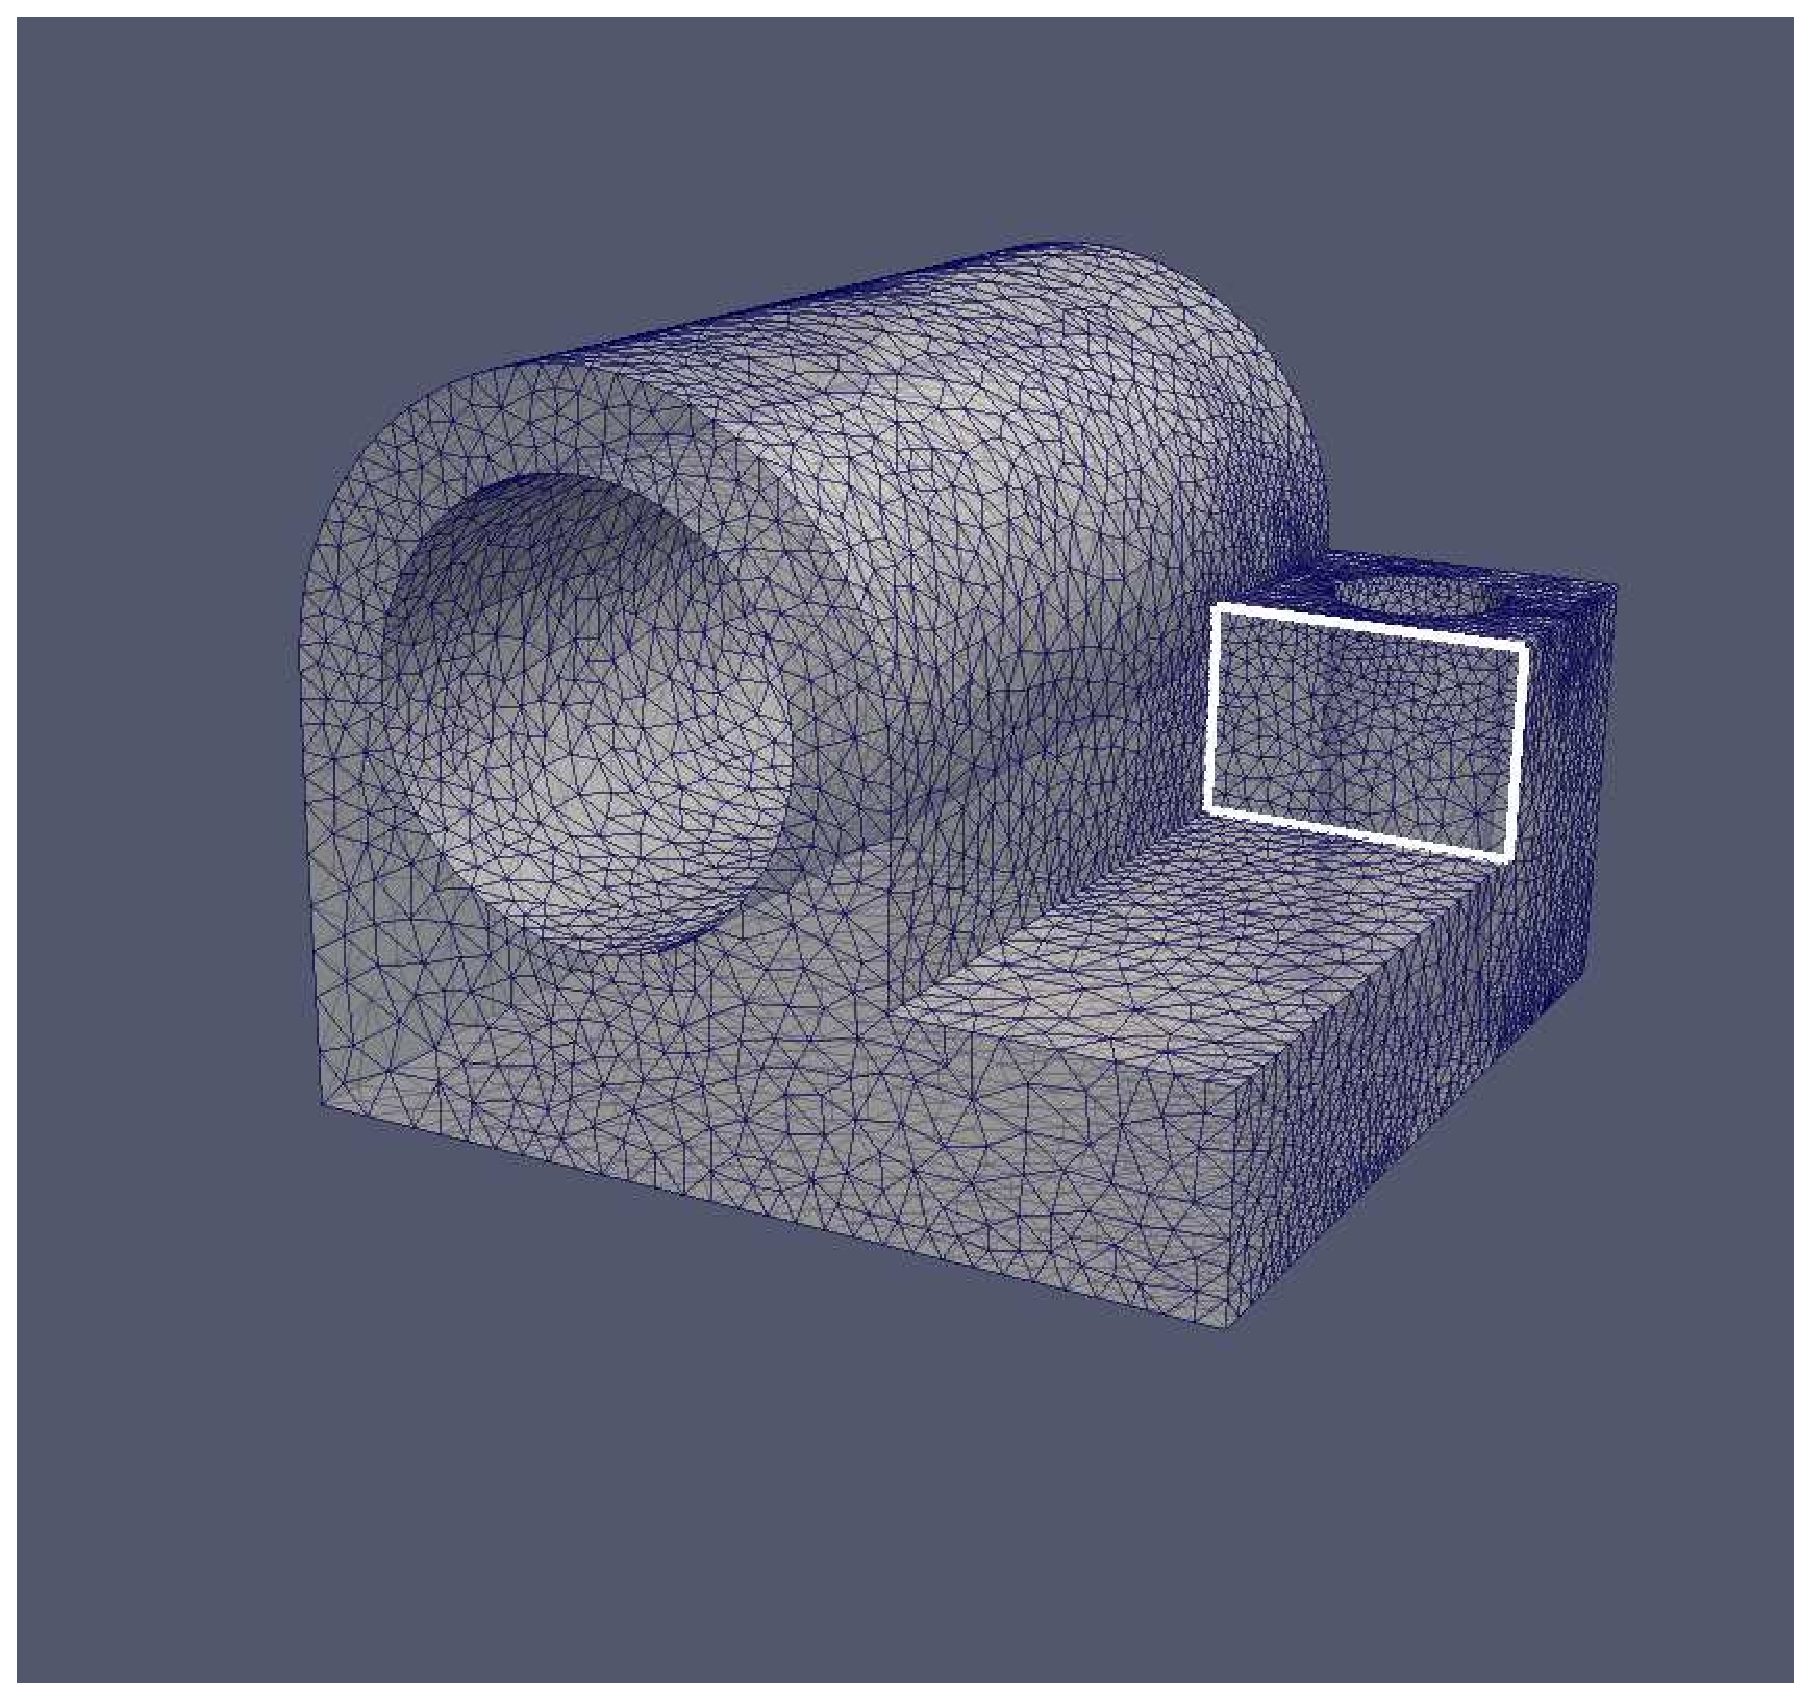
\includegraphics[width=.8\linewidth]{surface-segmentation/surf0.eps}
  \caption{}
  \label{surf0}
\end{subfigure}%
\begin{subfigure}{.5\textwidth}
  \centering
  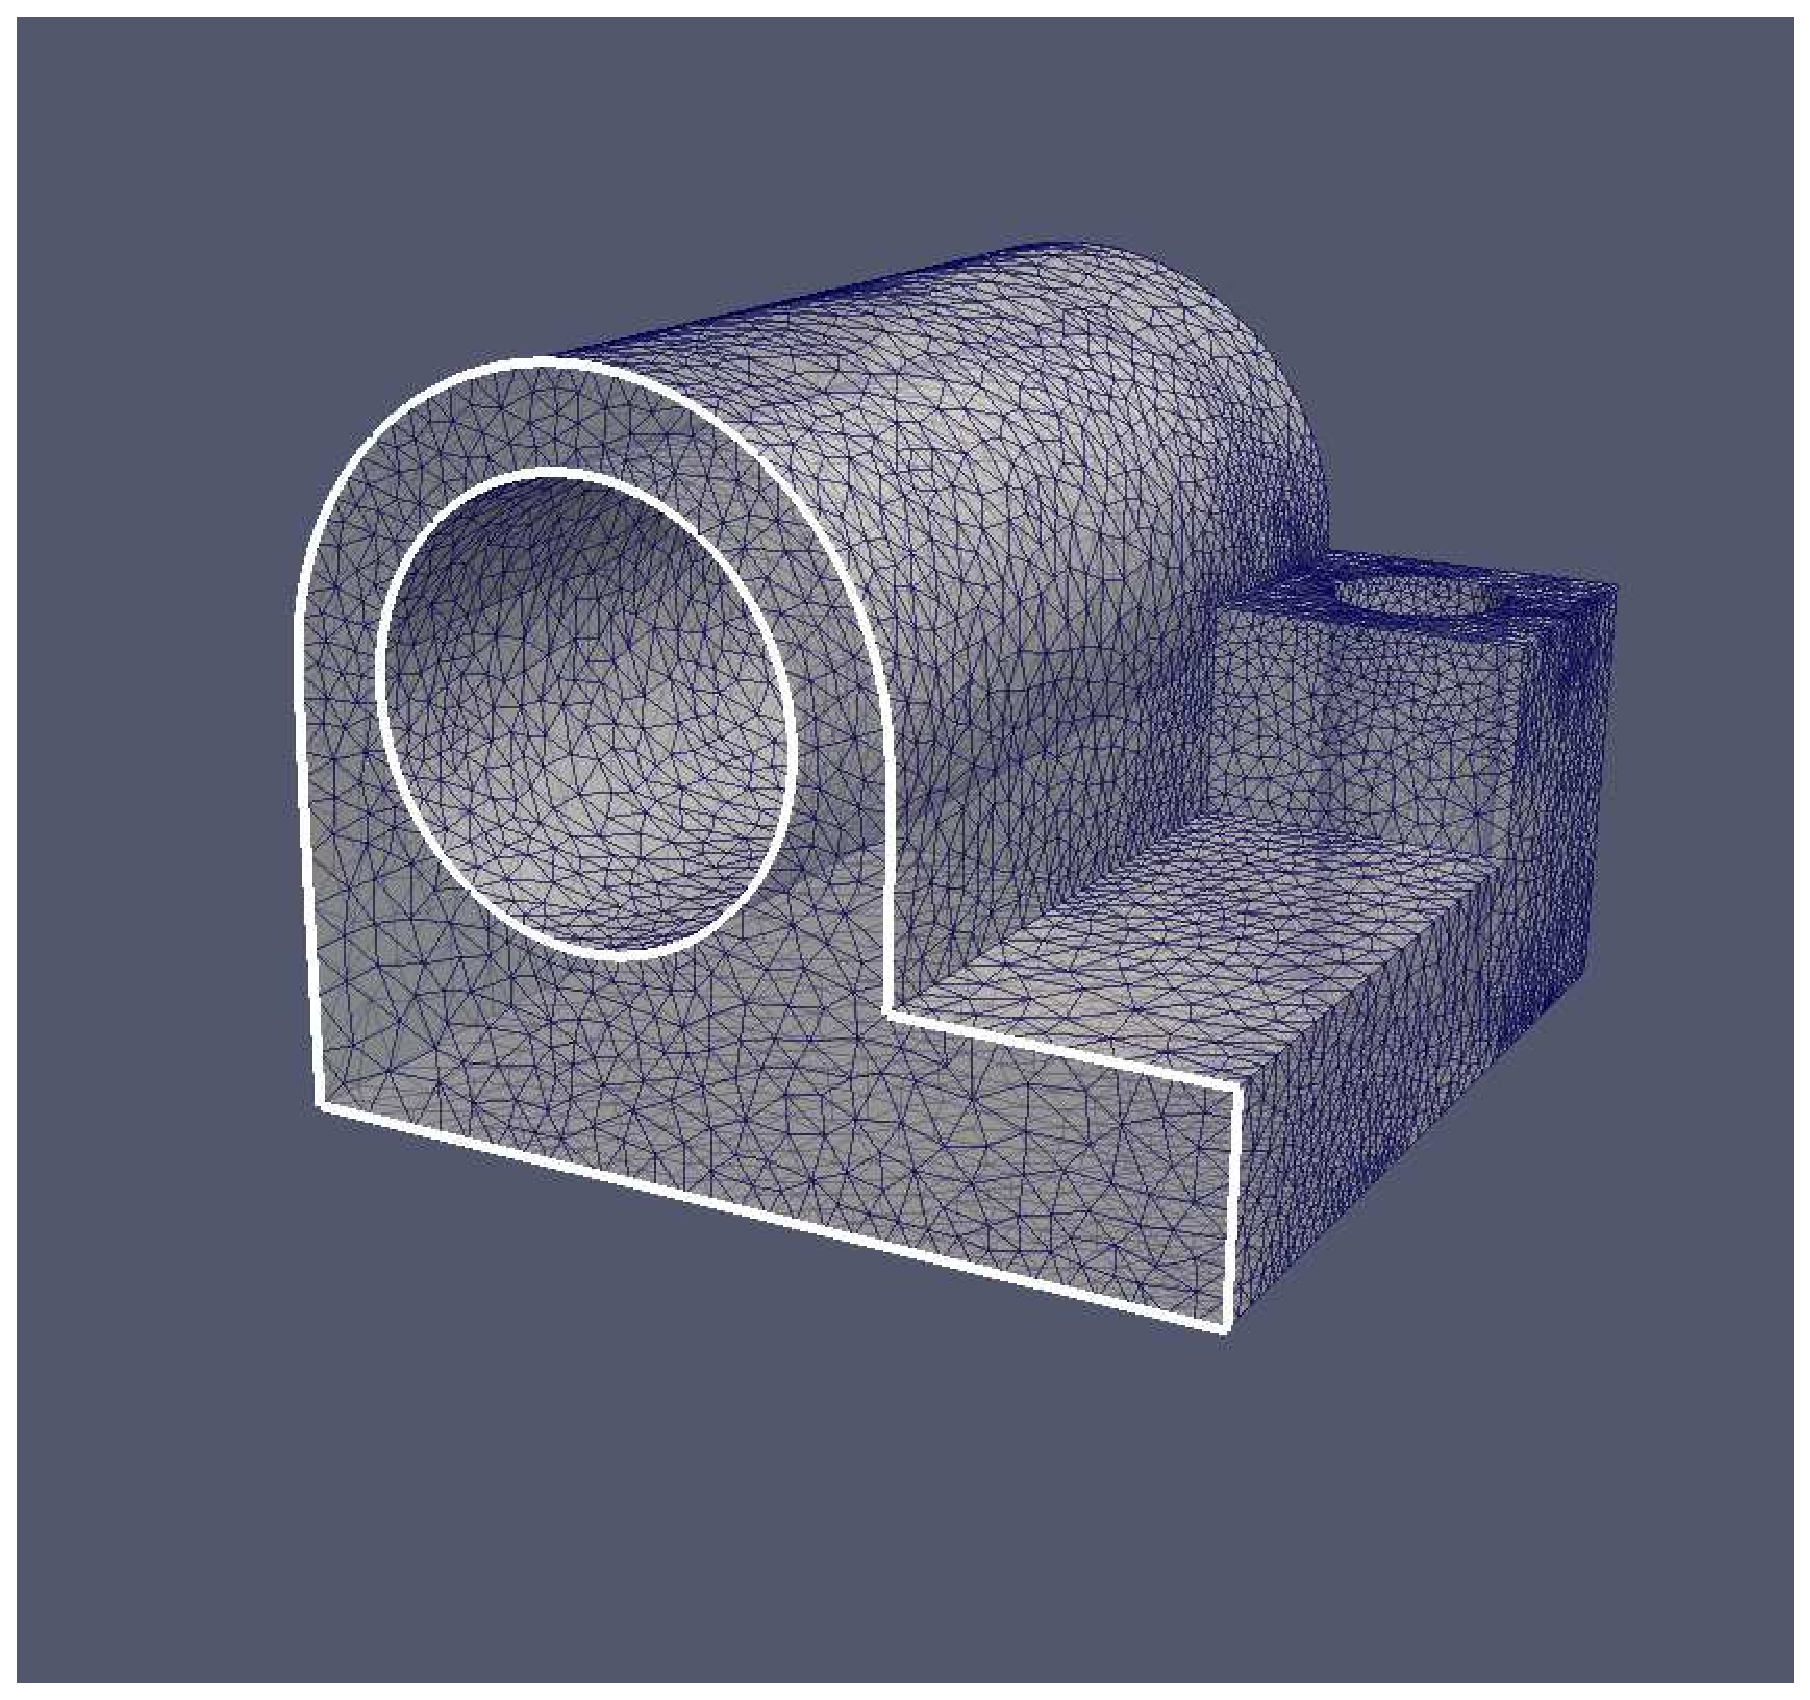
\includegraphics[width=.8\linewidth]{surface-segmentation/surf3.eps}
  \caption{}
  \label{surf1}
\end{subfigure}
\begin{subfigure}{.5\textwidth}
  \centering
  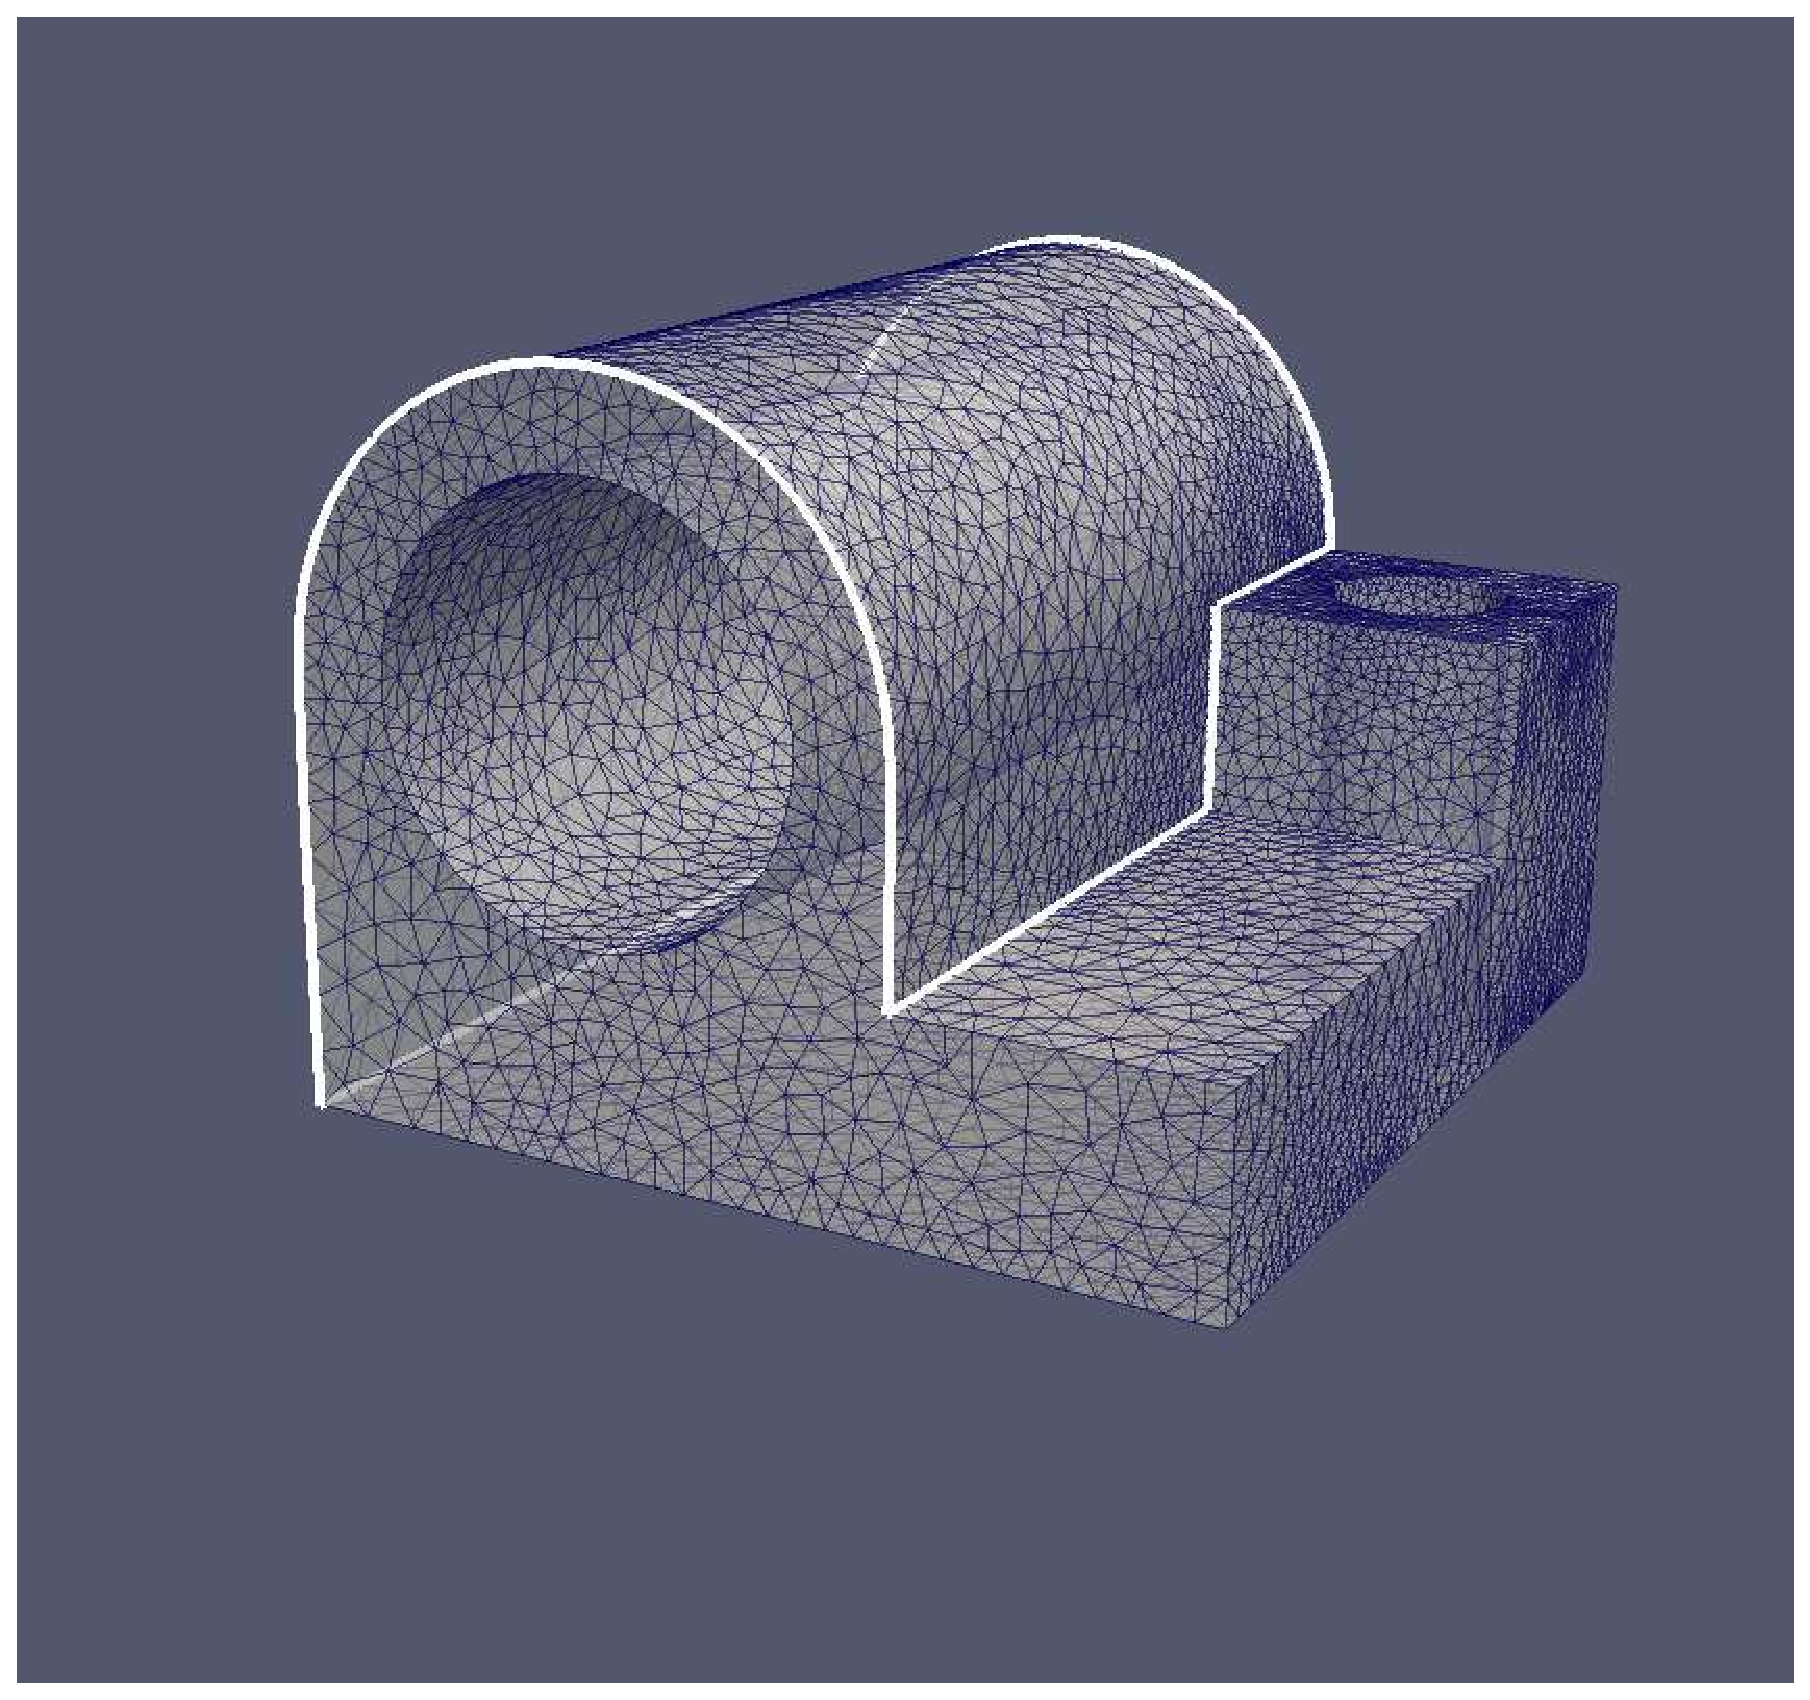
\includegraphics[width=.8\linewidth]{surface-segmentation/surf5.eps}
  \caption{}
  \label{surf2}
\end{subfigure}%
\begin{subfigure}{.5\textwidth}
  \centering
  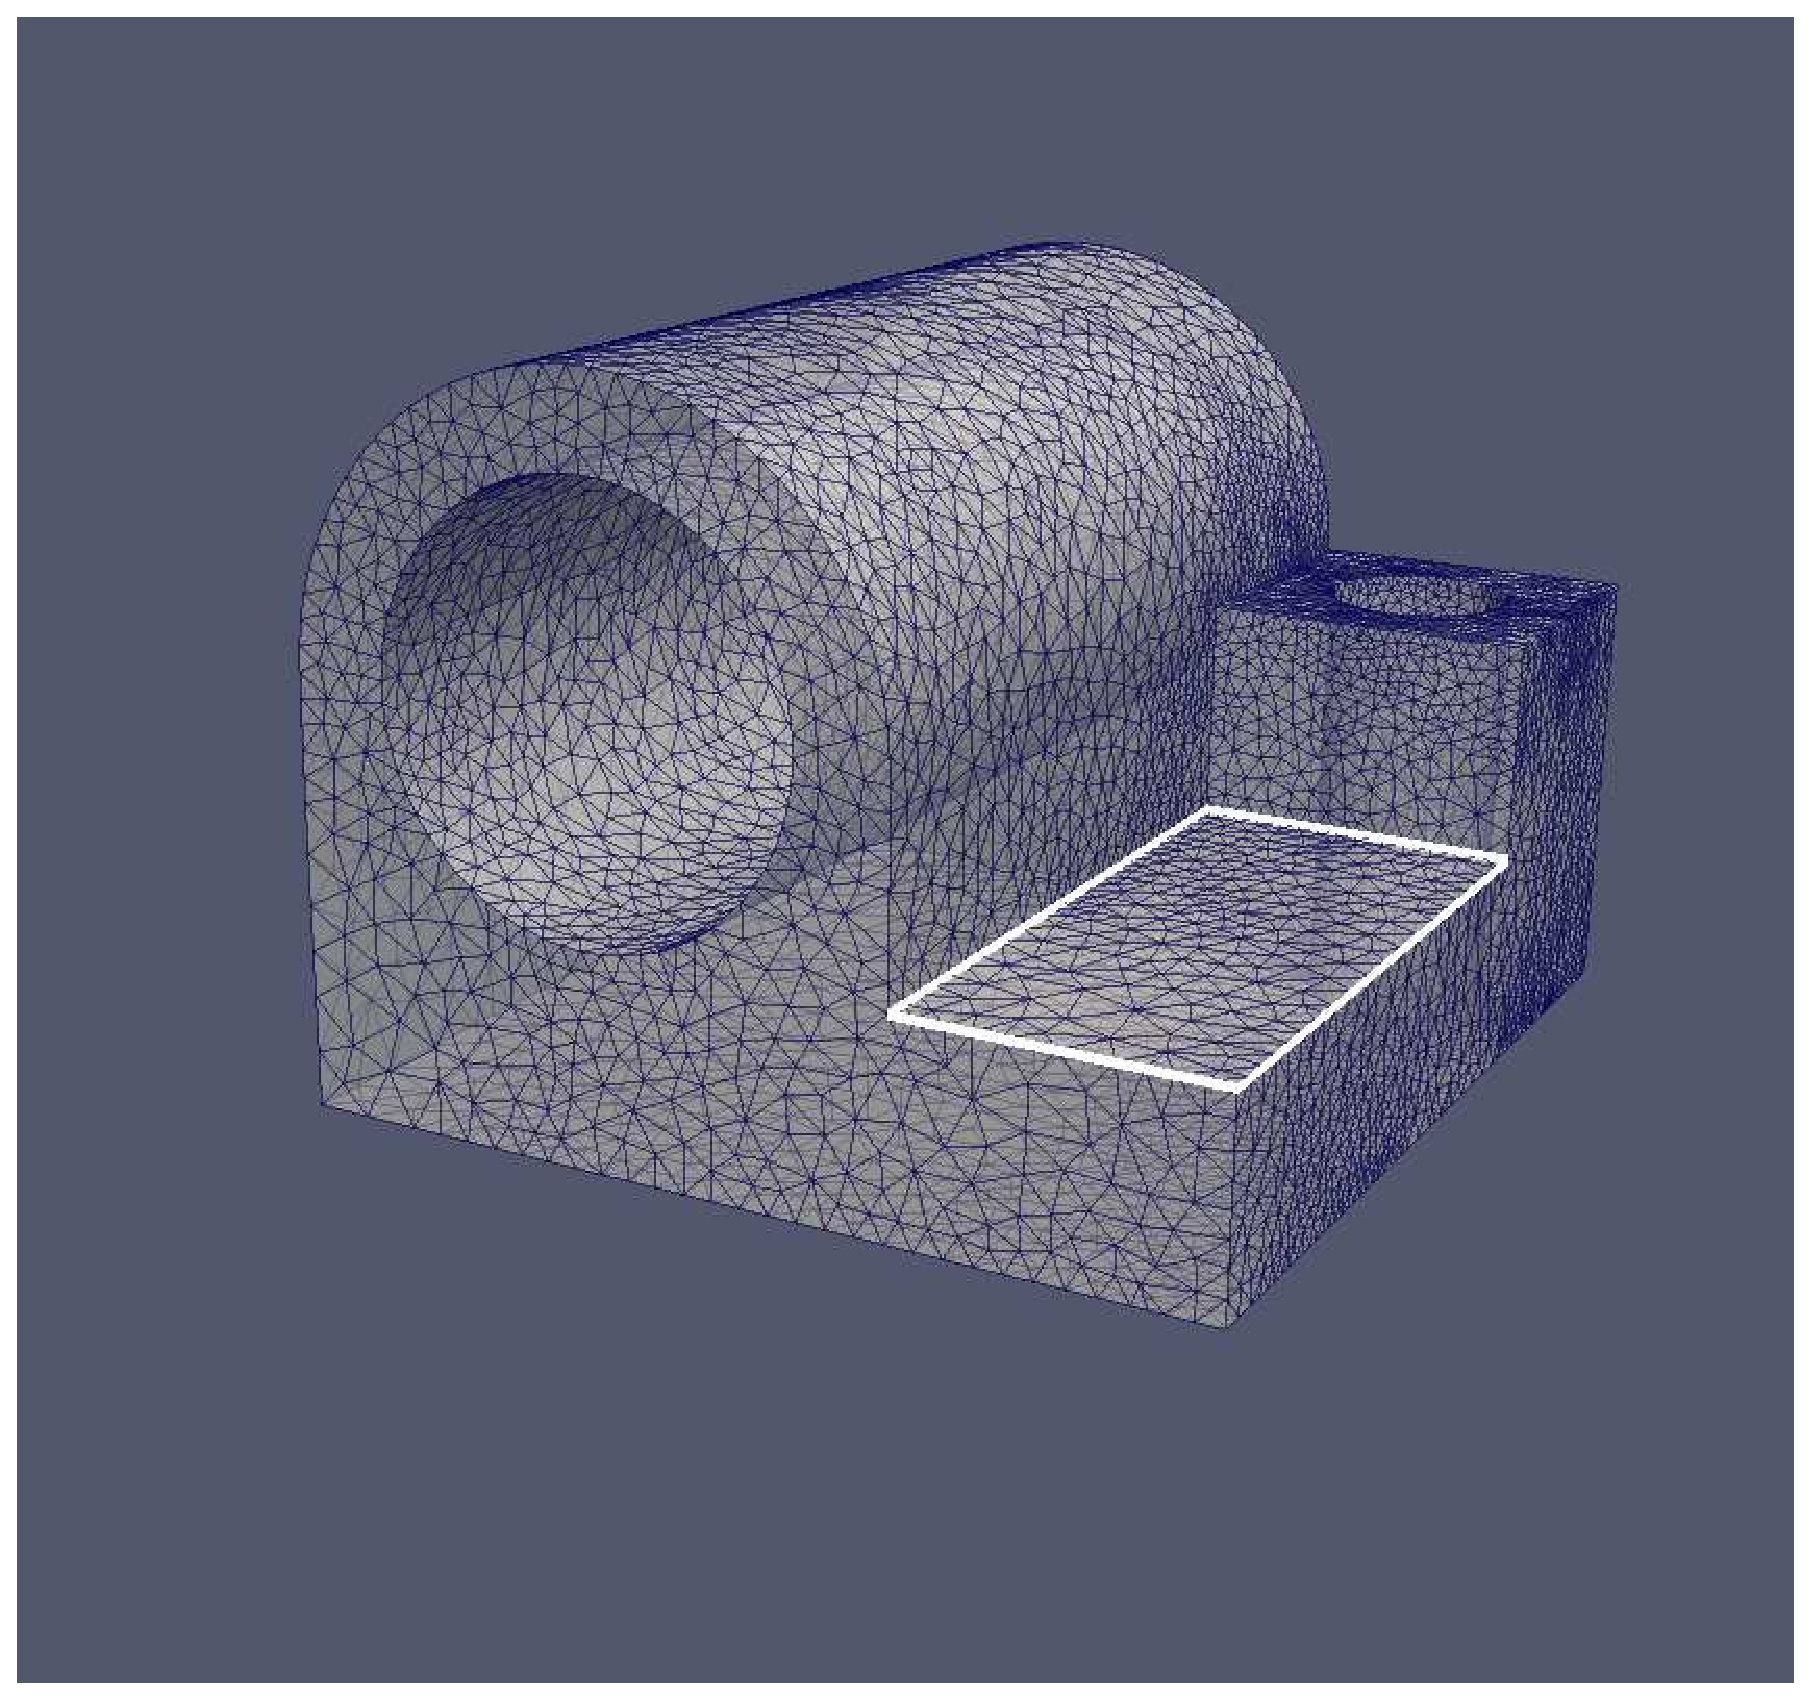
\includegraphics[width=.8\linewidth]{surface-segmentation/surf7.eps}
  \caption{}
  \label{surf3}
\end{subfigure}
\caption{An example input triangulation with some of the segmented surfaces.}
\label{surf-segment}
\end{figure}

\subsection{Boundary Initialization}

After importing the surface triangulation, we have a valid underlying surface representation with us. Also, segmented sub-surfaces and their boundaries provide us with the boundary we need to march off of. The mesh generation routine starts by initializing the boundaries of each sub-surface of the surface by marking each point on the boundary as a candidate marching point which form the starting layer in the mesh. The points at the boundary of the mesh serve as the parent points for the first layer inserted into the mesh. The data structure for each boundary front vertex stores its adjacent edges so as to identify the marching directions which is explained in detail in the next subsection. Each edge stores the direction into the interior of the sub-surface it bounds with respect to the surface normal. As the sub-segments sharing a common boundary are meshed independently, it is easier to identify the normal to an edge along the sub-surface for advancing the front in the mesh generation algorithm.

\subsection{Advancing Layer Routine- Point placement} \label{advancing-layer}

For each of the sub-surfaces of the geometry, the advancing layer routine iteratively picks a point from its boundary and extrudes it in a given direction. After evaluating the extruded point, we project the point onto the underlying surface. This process is set up to be of two steps for simplicity, accuracy and computational efficiency as will be explained later.

\begin{figure}[hbt!]
\centering
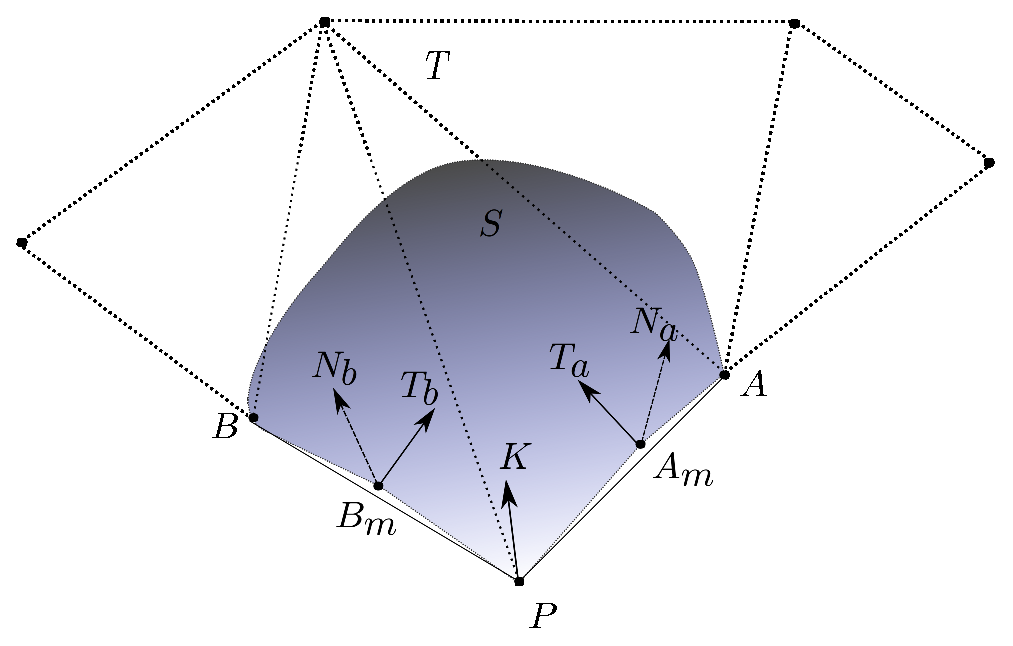
\includegraphics[width=.5\textwidth]{drawing-extrude-direction.eps}
\caption{Calculation of the extrude direction for a point P in the advancing front}
\label{extrude-direction}
\end{figure}

In the first step, we extrude the parent point to get the extruded point. We would interchangeably call the extruded points as the kid points as they represent the successors of their parent points from the previous layer. The direction of this extrusion is set up to be the average of the normals of the parent vertex's adjacent edges in the tangential plane of the sub-surface. In other words, the normals of the adjacent two edges of a vertex on the underlying sub-surface are averaged to get the extrusion direction. Consider Figure \ref{extrude-direction}; we need to find the extrusion direction of a point P on the boundary. In the underlying triangulation $T$, $PB$ and $PA$ are the edges adjacent to $P$ on the boundary of the surface $S$. We first find the points $B_m$ and $A_m$, which are the mid-points of quartic-bezier curves $PB$ and $PA$ which are constructed by CGM as a part of constructing the quartic-bezier triangular surface patches from the underlying triangulation $T$. Next, we find the normal directions on the surface at point $B_m$ and $A_m$ which are labeled as $N_b$ and $N_a$ in the figure. We cross product the vector $PB$ with $N_b$ to get the direction $T_b$. The vector $T_b$ is normal to the edge $PB$ as well as tangential to the surface $S$. Similarly, we find the vector $T_a$. The direction of extrusion $PK$ is chosen to be the average of the direction of $T_a$ and $T_b$.

The initial extrusion length is an input parameter provided by the user. This length would be taken as the extrusion length when the boundary points are extruded for the first time to the interior of the surface. This length can vary with boundary vertices as the points are extruded independently. Hence, this extrude length can either be supplied by the user for all the points of the boundary separately or as a single value for all the boundary points. To get the best quality of quad elements, we are also experimenting with a varying extrude length along the boundary with respect to the interior angle between the direction vectors $T_a$ and $T_b$. If the vertex is a concave corner vertex, the extrude length is increased so as to create good quality quad elements in the next layer and vice-versa for convex corner vertices. Also, if the vertex is a convex corner, additional marching directions are added so as to sufficiently refine the interior domain of the surface. The number of additional marching directions added depends on the convexity of the vertex. If we have $n$ marching directions for a point, the angle between the adjacent edges would be divided into $n+1$ angles to get the marching directions for the $n$ points. We hope to include these modifications in the final paper submission.

After we have extruded the point, we project it on to the underlying geometry. This operation ensures that all the  points we insert in the mesh are on the underlying geometry and avoid compounding the errors in subsequent layer generation process. Points are inserted in the mesh and the mesh elements are subdivided to include the new point. The candidate point for insertion can subdivide an existing triangle to replace the previous triangle with three new ones, or can subdivide an edge to replace existing two triangles with four new ones. To find the best triangle or edge for subdivision, we first make a guess for the triangle to insert the point. Any triangle in the surface interior adjacent to the point being extruded is chosen. Starting from this triangle, we iteratively jump to the best edge or triangle by comparing the barycentric coordinates of the new point with respect to the triangle in consideration. This technique suffers from two disadvantages. First, we need to compare double precision values of barycentric coordinates for making a decision on which triangle to choose for insertion. If the values are too close, the point might be inserted in the wrong triangle and would eventually lead to deviation of the mesh from the underlying surface. Second, the process of iteratively finding the right triangle for insertion might end up being in an infinite loop. Both of these problems are substantially reduced with a good isotropic initial triangulation. However, we add several validation tests to avoid these problems even for a coarse initial triangulation. These include orientation checks of the triangles formed with respect to the surface, thresholding the maximum deviation of the newly formed triangle from the surface and thresholding the dihedral angles between two triangles on the surface. We use an epsilon value of $10^{-5}$ while comparing the values of barycentric coordinates to zero. Also, we insert the point on a face rather than in a triangle when the ratio of the second-smallest barycentric coordinate to the smallest one is more than a set threshold($10^2$). This helps us avoid very skinny triangles with large obtuse angles and also helps in avoiding several unnecessary face swapping in the mesh.

After advancing one layer to the surface interior, we increase the extrude length at each point by a factor. This factor, called the growth ratio would specify the anisotropic layer-on-layer extrusion length growth as we march on the surface. A value of growth ratio between 1.1 and 1.4 gives us satisfactory anisotropy at the boundaries of the mesh.

\begin{figure}[hbt!]
    \centering
    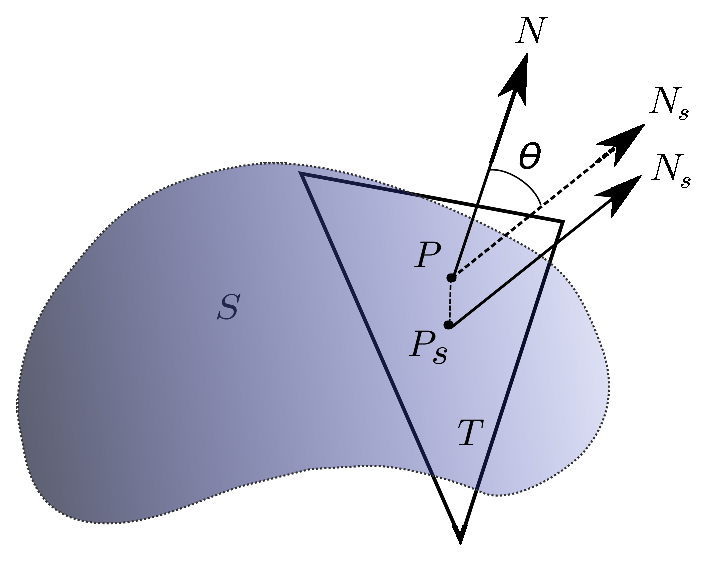
\includegraphics[width=.3\textwidth]{deviate-surface.eps}
    \caption{Triangle $T$ deviates from the underlying surface $S$. $P$ is the centroid of $T$ and $P_s$ is the projection of $P$ on $S$. The deviation is calculated as the interior angle between the normal to the triangle $PN$ and the normal to the surface at $P_s$, which is $P_sN_s$. The angle $\theta$ represents the deviation here. The deviation is exaggerated for illustration purposes.}
    \label{deviation-surface}
\end{figure}

\subsection{Local Reconnection for quality}

A mesh observer object is initialized for the mesh data structure. The observer monitors all the changes happening to the mesh. These include creation and deletion of vertices, edges and cells in the mesh. An edge swapping manager and quality criterion for deciding a swap are also initialized for the mesh. The primary quality criterion we chose for an edge swap is maximization of the minimum angle in the pair of triangles adjacent to the edge before and after the swap. However, only this criterion is not enough for improving surface mesh quality. This is because a better quality pair of triangles may result by edge swapping according to this criterion, however, they might deviate quite a bit from the underlying surface. Hence, we threshold the maximum deviation of the resultant triangles from the surface. This deviation is calculated as the angle between the normal to the triangle and the normal at the centriod of the triangle projected onto the surface. See Figure \ref{deviation-surface} for reference. Deviation of a triangle $T$ with respect to a surface $S$ is shown. $P$ is the centroid of the triangle and $P_s$ is the projection of the centroid onto the surface. $PN$ is the normal to the triangle and $P_sN_s$ is the normal to the surface at $P_s$. The interior angle $\theta$ is considered as the deviation of the triangle from the surface. A upper bound is set for $\theta$ to limit the deviation of resultant triangles from the surface.  The bound is set to $\ang{30}$ for the surfaces meshes we are dealing with. This bound is sensitive to the refinement in the initial triangulation. Basically, a higher value of $\theta$ would be apt for a coarse initial triangulation while the value can be set low for a fine initial triangulation.

We queue up the edges of the triangles affected by the insertion of the new point and do edge swapping for these edges to improve on the existing mesh. Figure \ref{point-insert} shows the process of point insertion and local reconnection in two steps. First, a point is inserted into the mesh at the desired location. This results in subdivision of a triangle as can be seen in figure \ref{point-insert2}. Subsequently, edge swaps occur to improve the mesh quality. Two iterations of edge swap can be seen in figure \ref{point-insert3} and \ref{point-insert4}. We do not swap the edges which comprise the front or the edge between parent and child points. Doing so would invalidate the advancing front. Hence, only interior faces of the surface or the diagonals of the quad elements generated are swapped by the face swapping algorithm. After edge swapping, the algorithm moves on to the next point in the current layer to repeat the same process.

\begin{figure}[hbt!]
\centering
\begin{subfigure}{.5\textwidth}
  \centering
  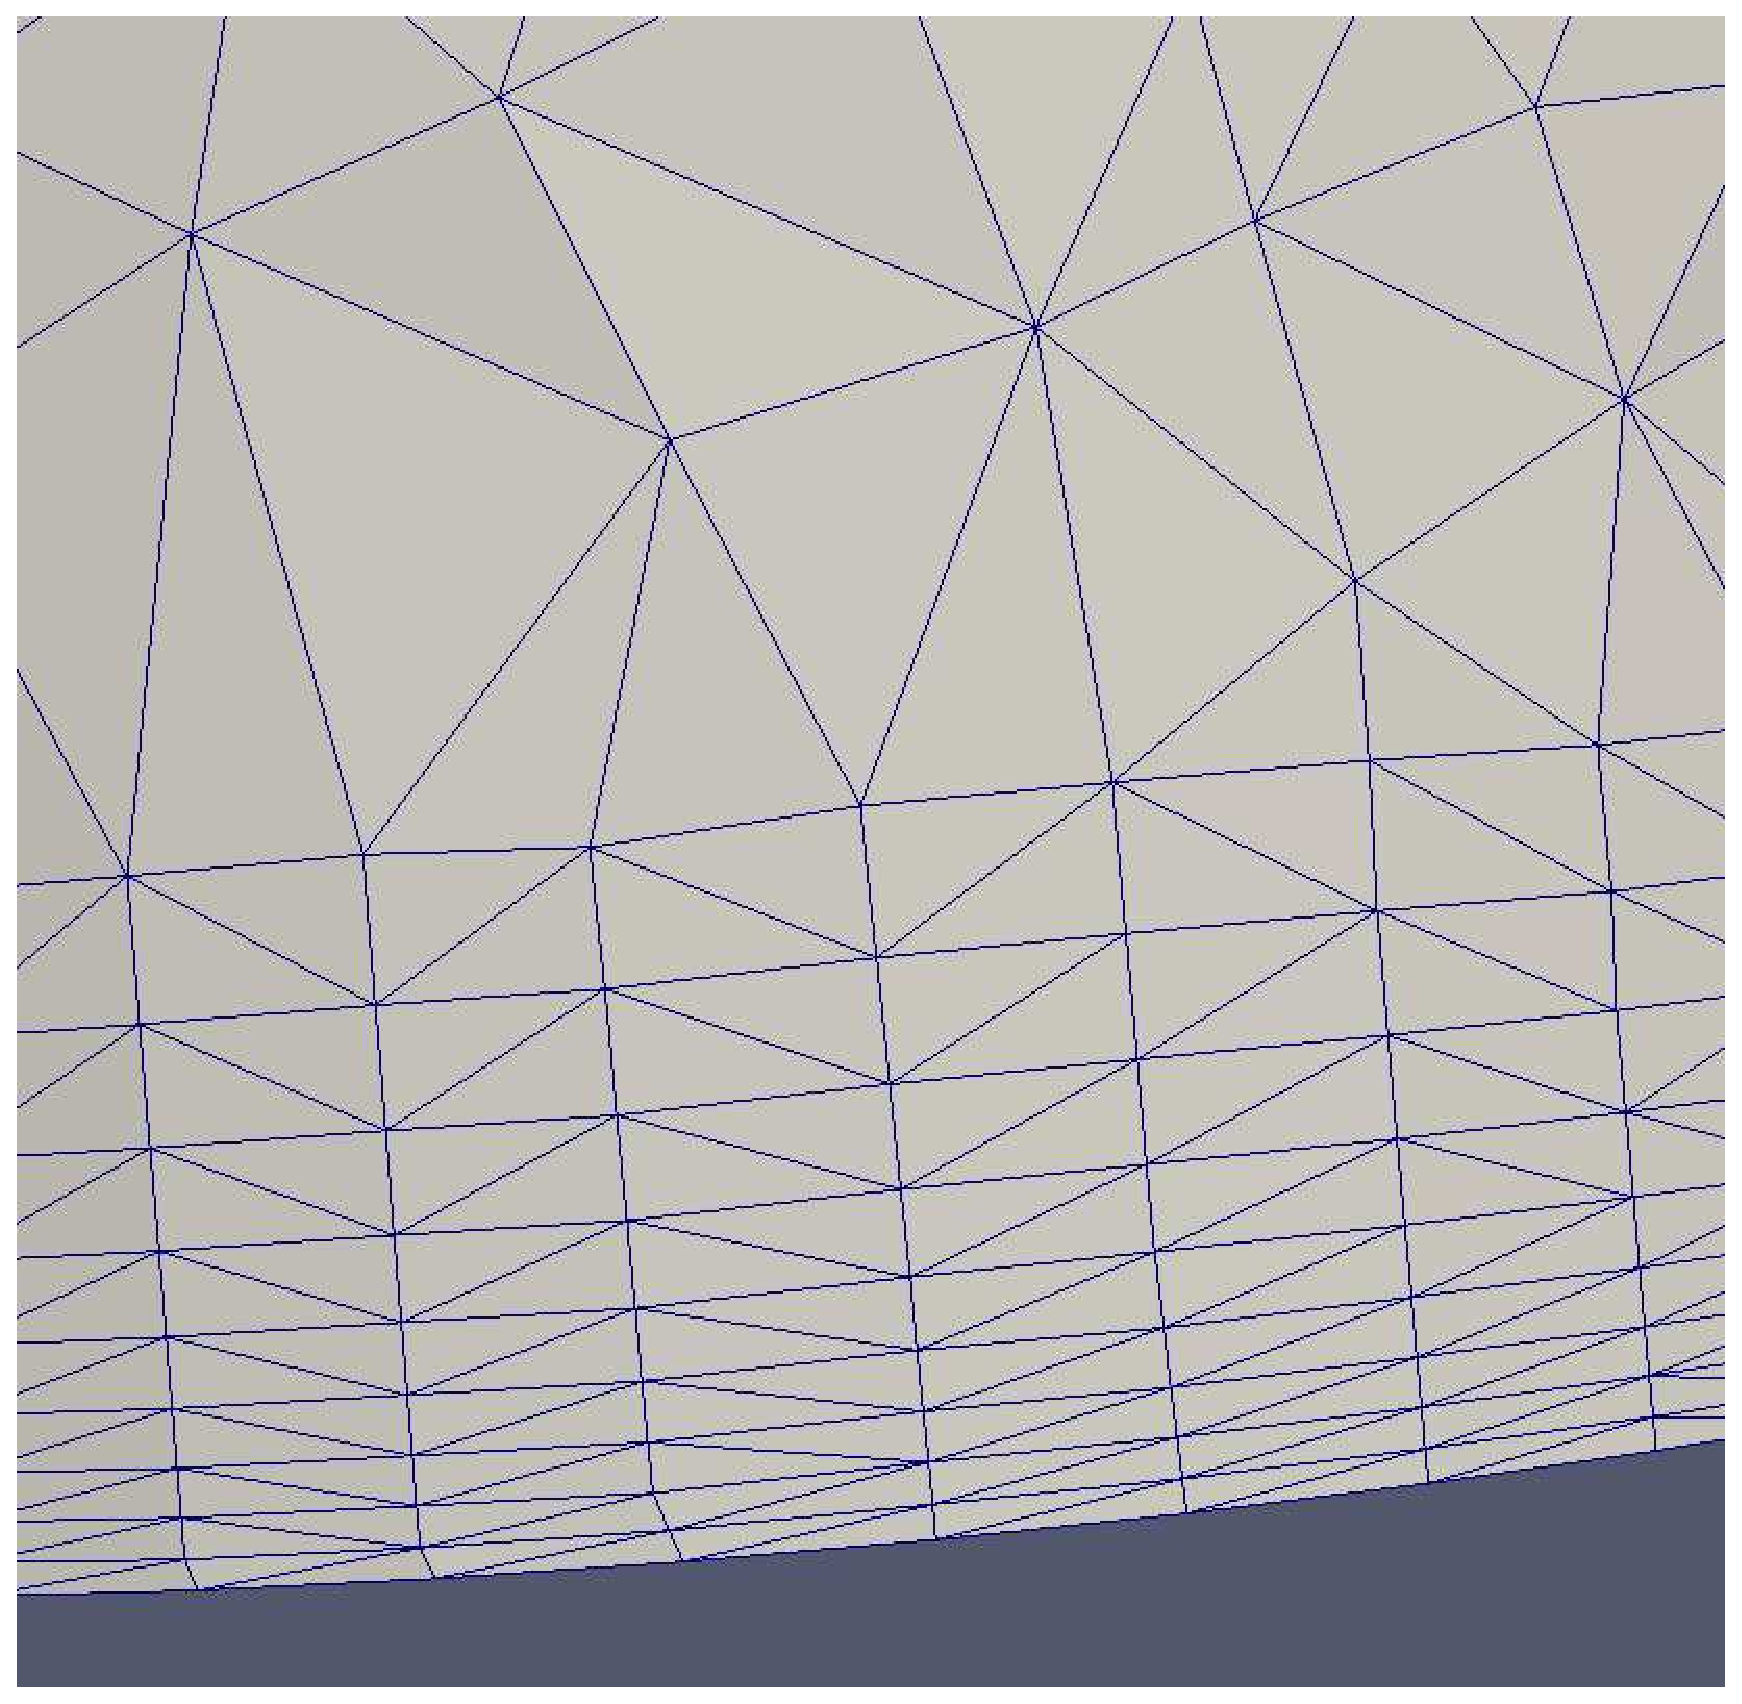
\includegraphics[width=.8\linewidth]{point-insertion-swapping/initial.eps}
  \caption{}
  \label{point-insert1}
\end{subfigure}%
\begin{subfigure}{.5\textwidth}
  \centering
  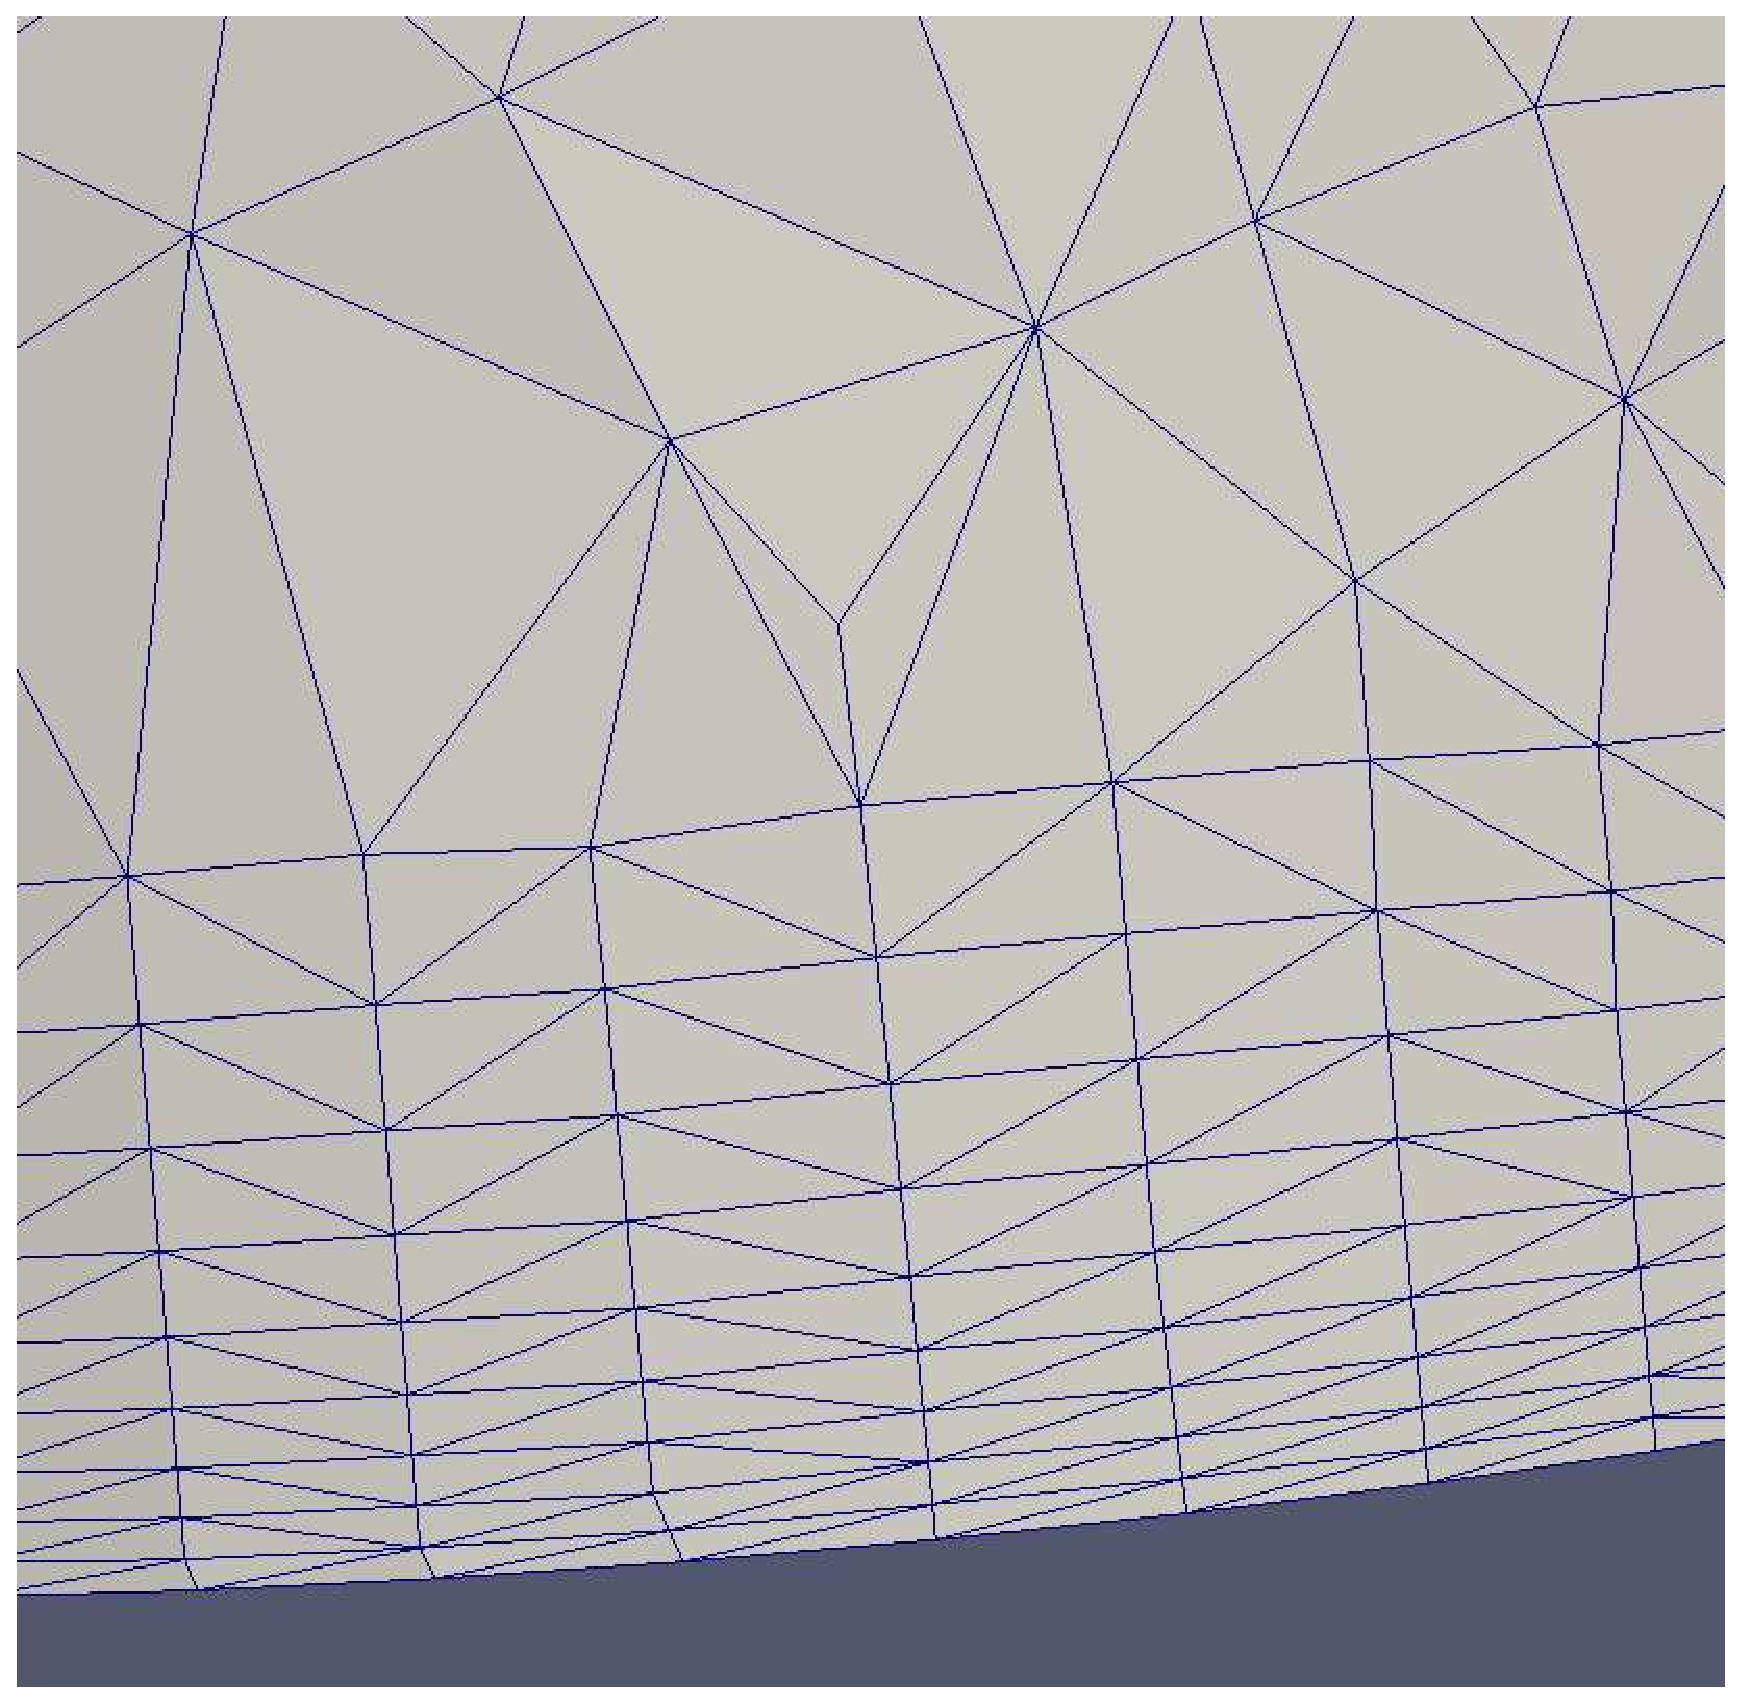
\includegraphics[width=.8\linewidth]{point-insertion-swapping/point-inserted.eps}
  \caption{}
  \label{point-insert2}
\end{subfigure}
\begin{subfigure}{.5\textwidth}
  \centering
  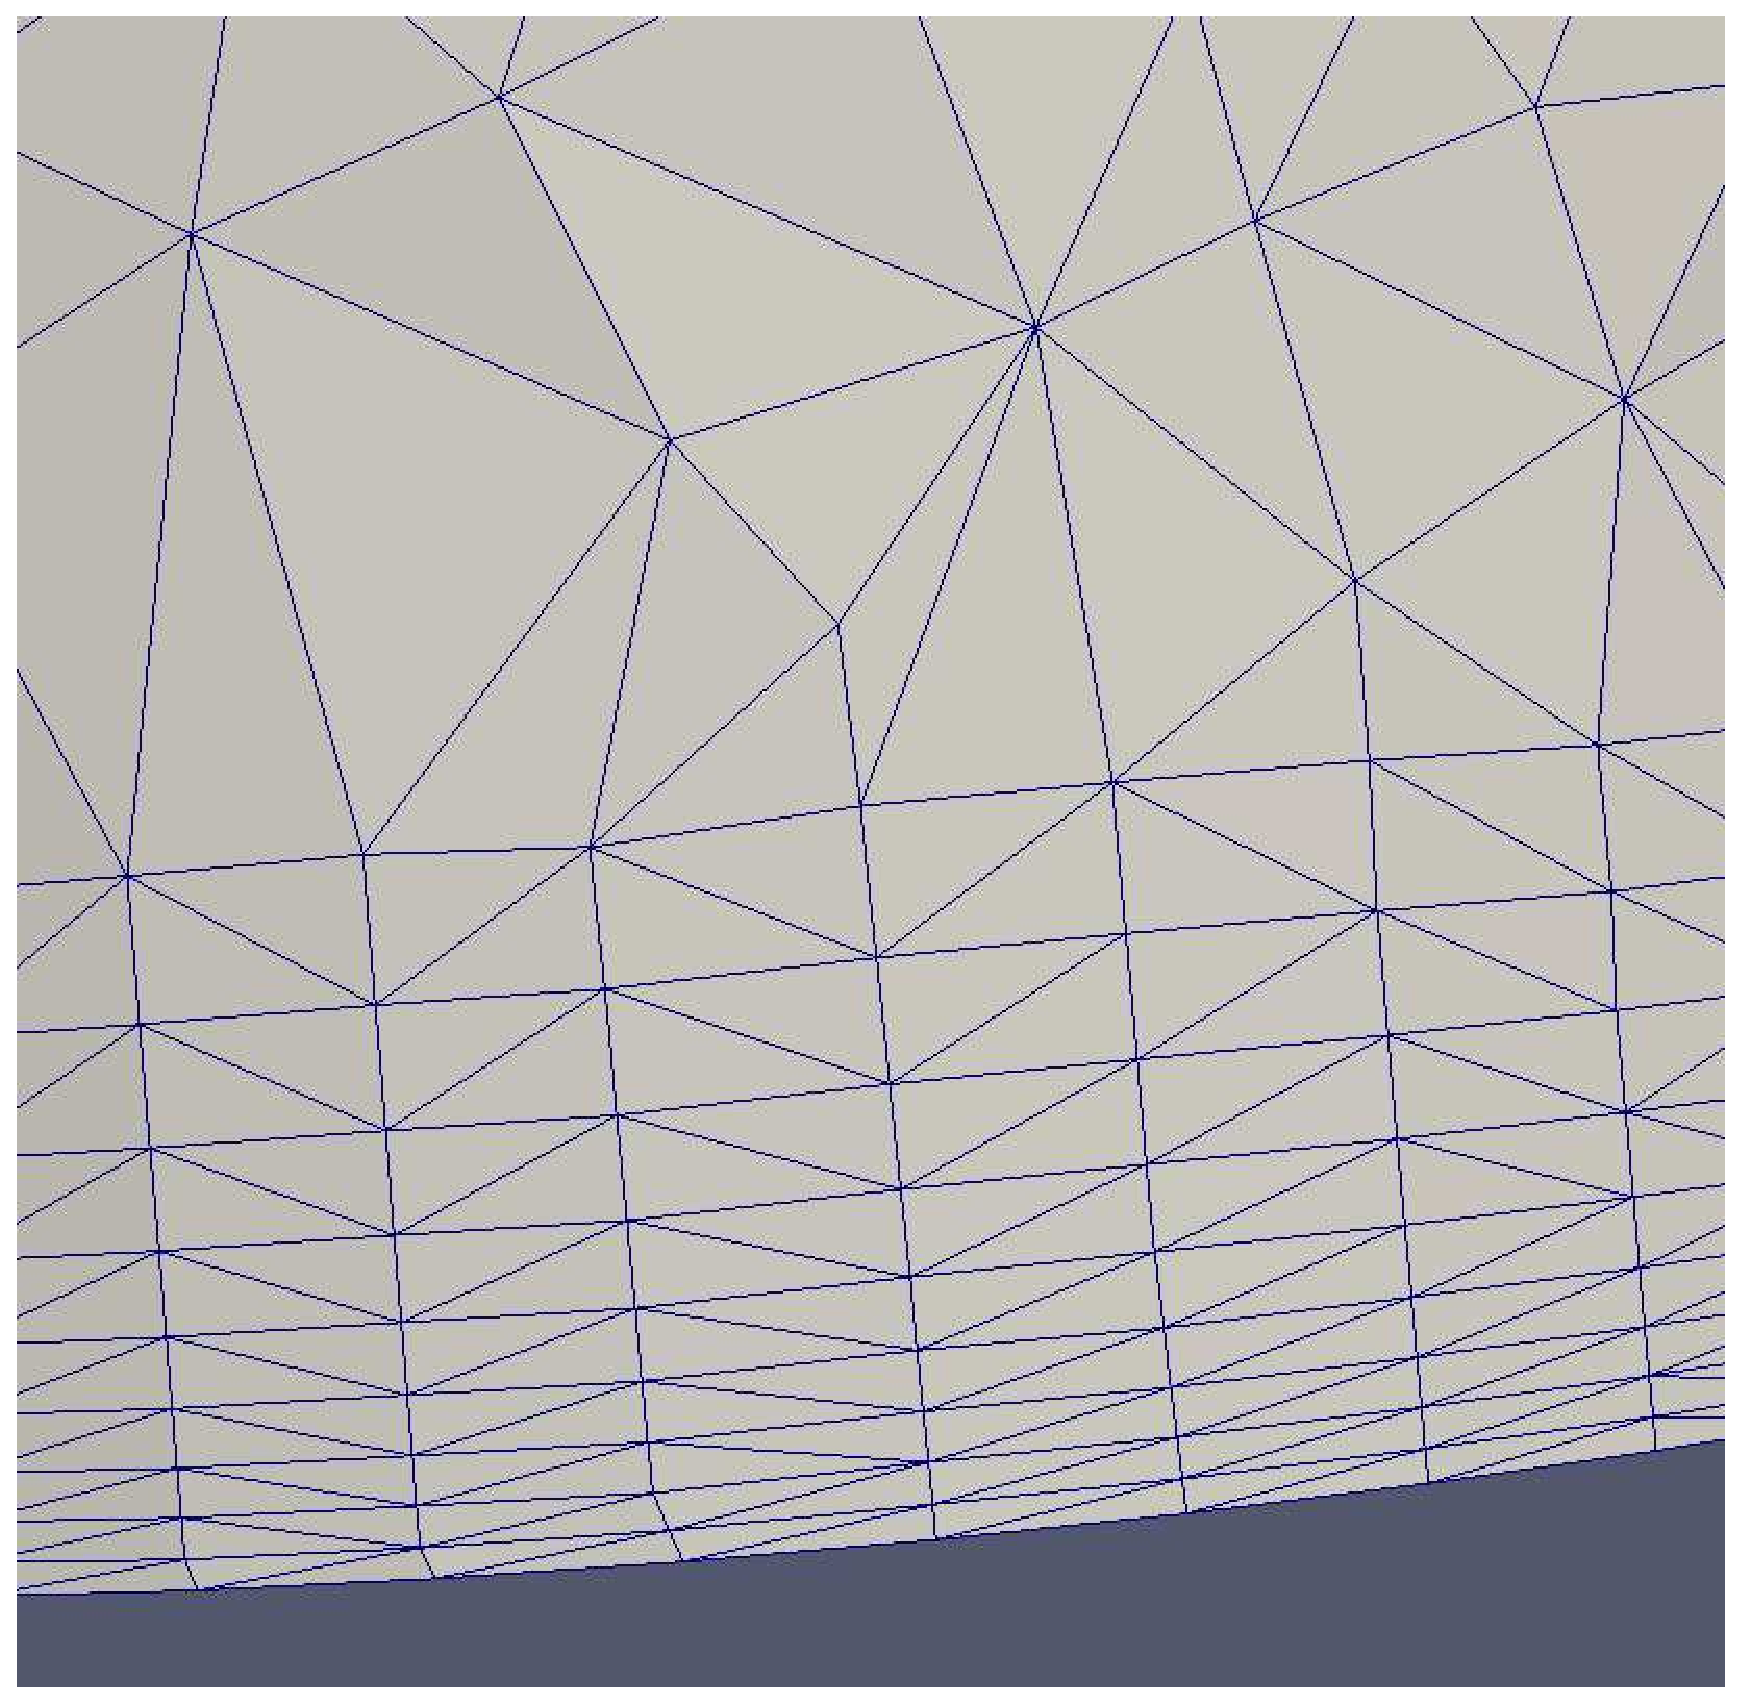
\includegraphics[width=.8\linewidth]{point-insertion-swapping/swap1.eps}
  \caption{}
  \label{point-insert3}
\end{subfigure}%
\begin{subfigure}{.5\textwidth}
  \centering
  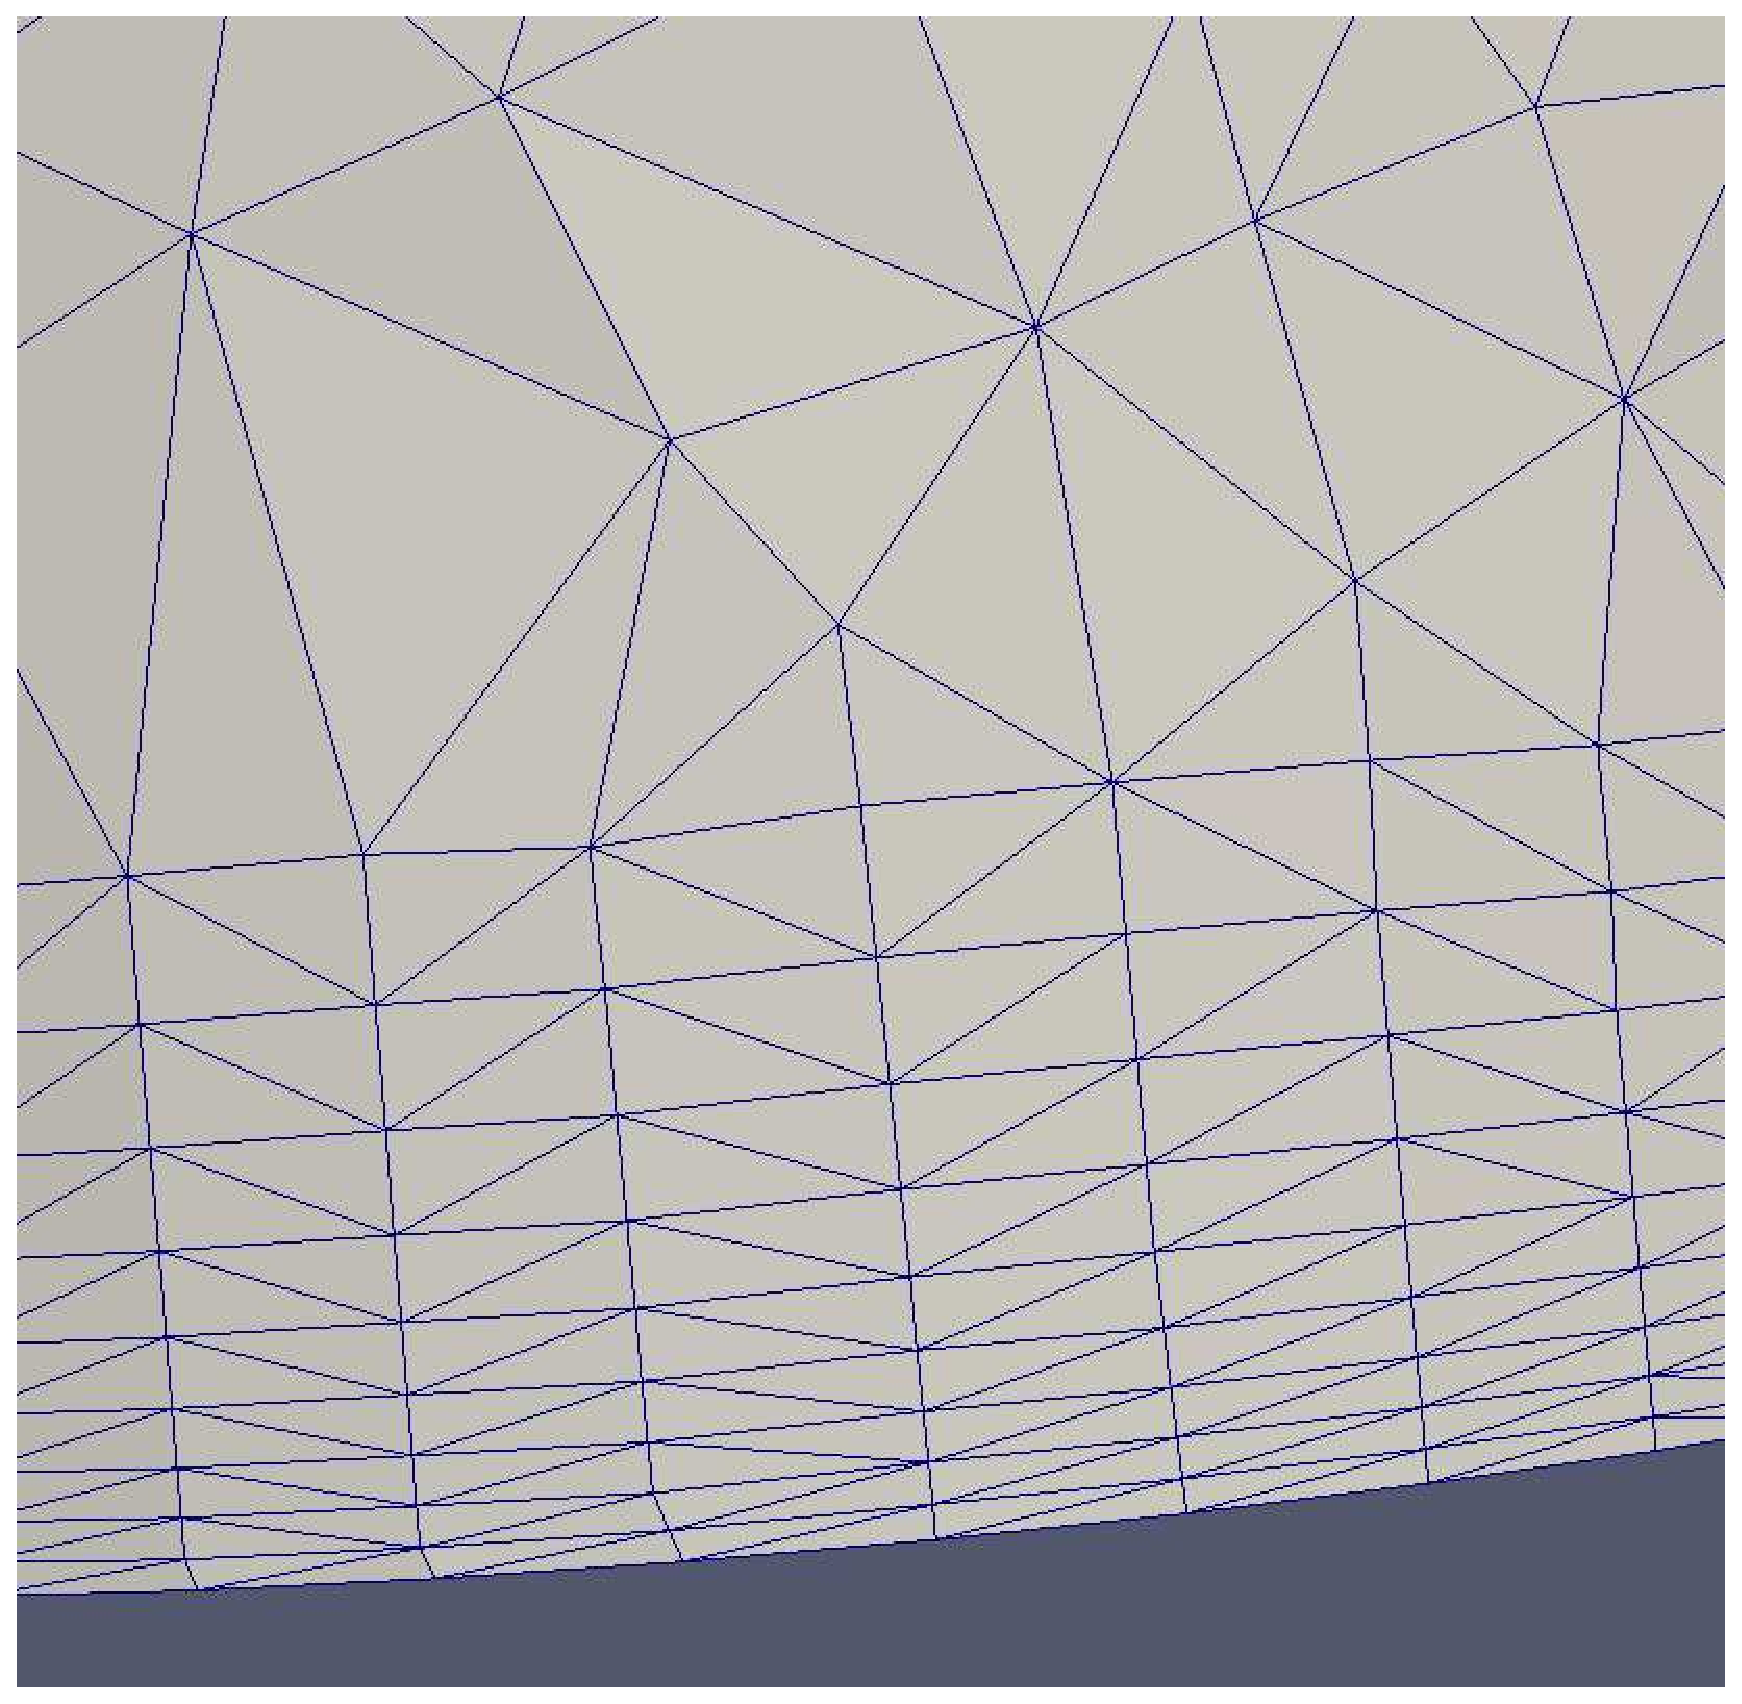
\includegraphics[width=.8\linewidth]{point-insertion-swapping/swap2.eps}
  \caption{}
  \label{point-insert4}
\end{subfigure}
\caption{Point Insertion and local reconnection for quality shown in four steps. (a) is the initial state of the mesh. A point is inserted in the mesh after extrusion from the parent point, projection onto the surface and finding the right triangle to insert. The triangle is subdivided into three new triangles as shown in (b). To improve the mesh quality after point insertion, swapping is done based on maximization of the minimum angle in a triangle. Two swaps occur as shown in figure (c) and (d) to improve mesh quality.}
\label{point-insert}
\end{figure}

\subsection{Front Recovery}

In an advancing layer mesh generation algorithm, the accurate representation of the boundary by anisotropic layers generated from it is very important. Also, generation of quad-elements from triangles with the right aspect ratios is far easier if we retain the boundary representation as we advance multiple layers. Hence, after all points of the parent layer are extruded, we implement a front recovery routine which recovers all edges between kid vertices.

\begin{figure}[hbt!]
\centering
\begin{subfigure}{0.5\textwidth}
  \centering
  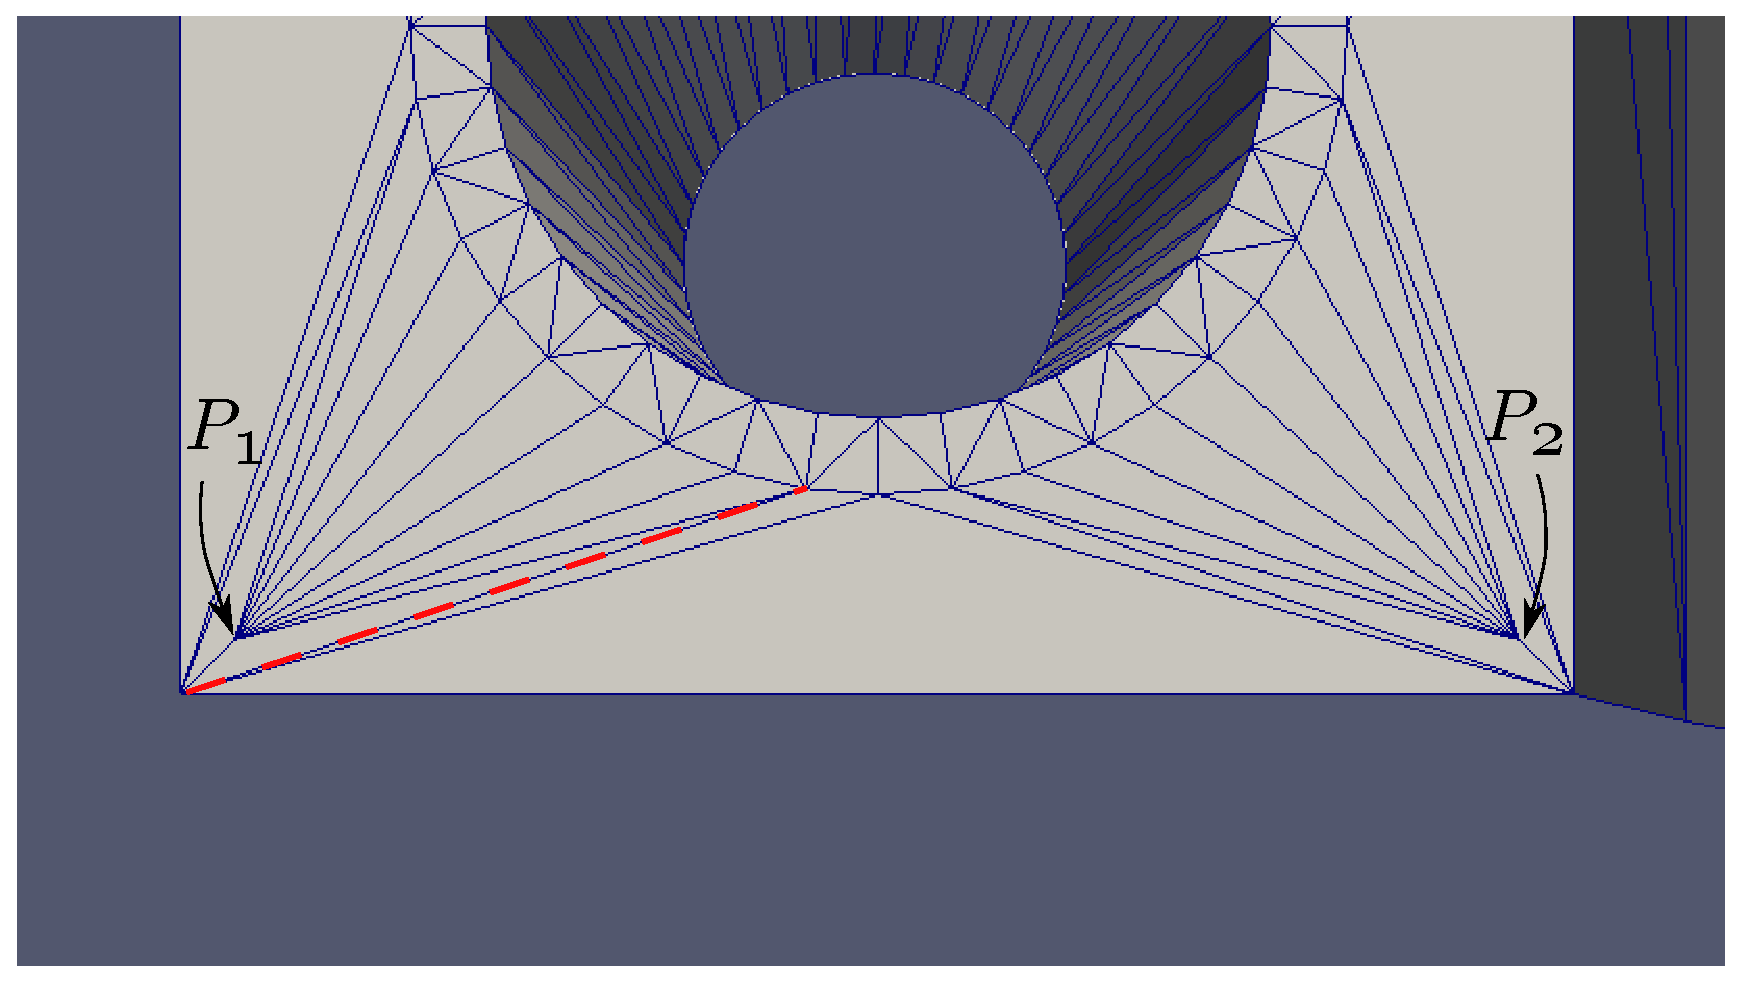
\includegraphics[width=.9\linewidth]{force-swapping-edge-recovery/initial-edited.eps}
  \caption{}
  \label{force-swap1}
\end{subfigure}%
\begin{subfigure}{.5\textwidth}
  \centering
  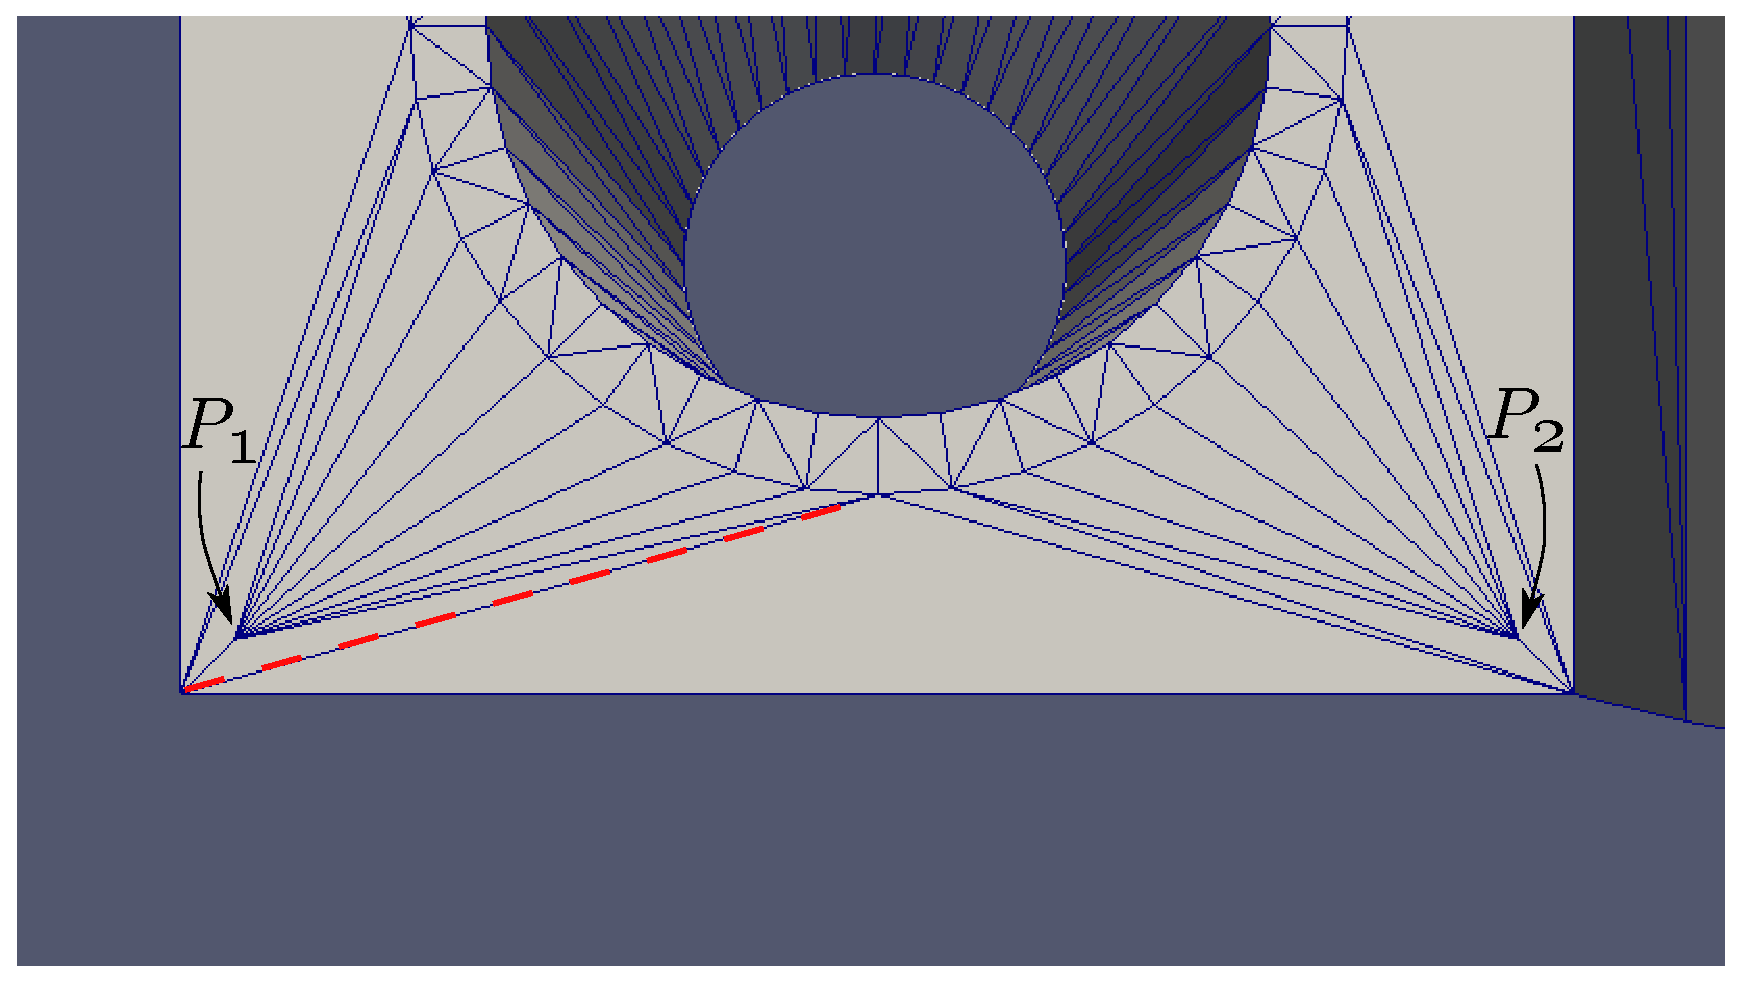
\includegraphics[width=.9\linewidth]{force-swapping-edge-recovery/swap1-edited.eps}
  \caption{}
  \label{force-swap2}
\end{subfigure}
\begin{subfigure}{.5\textwidth}
  \centering
  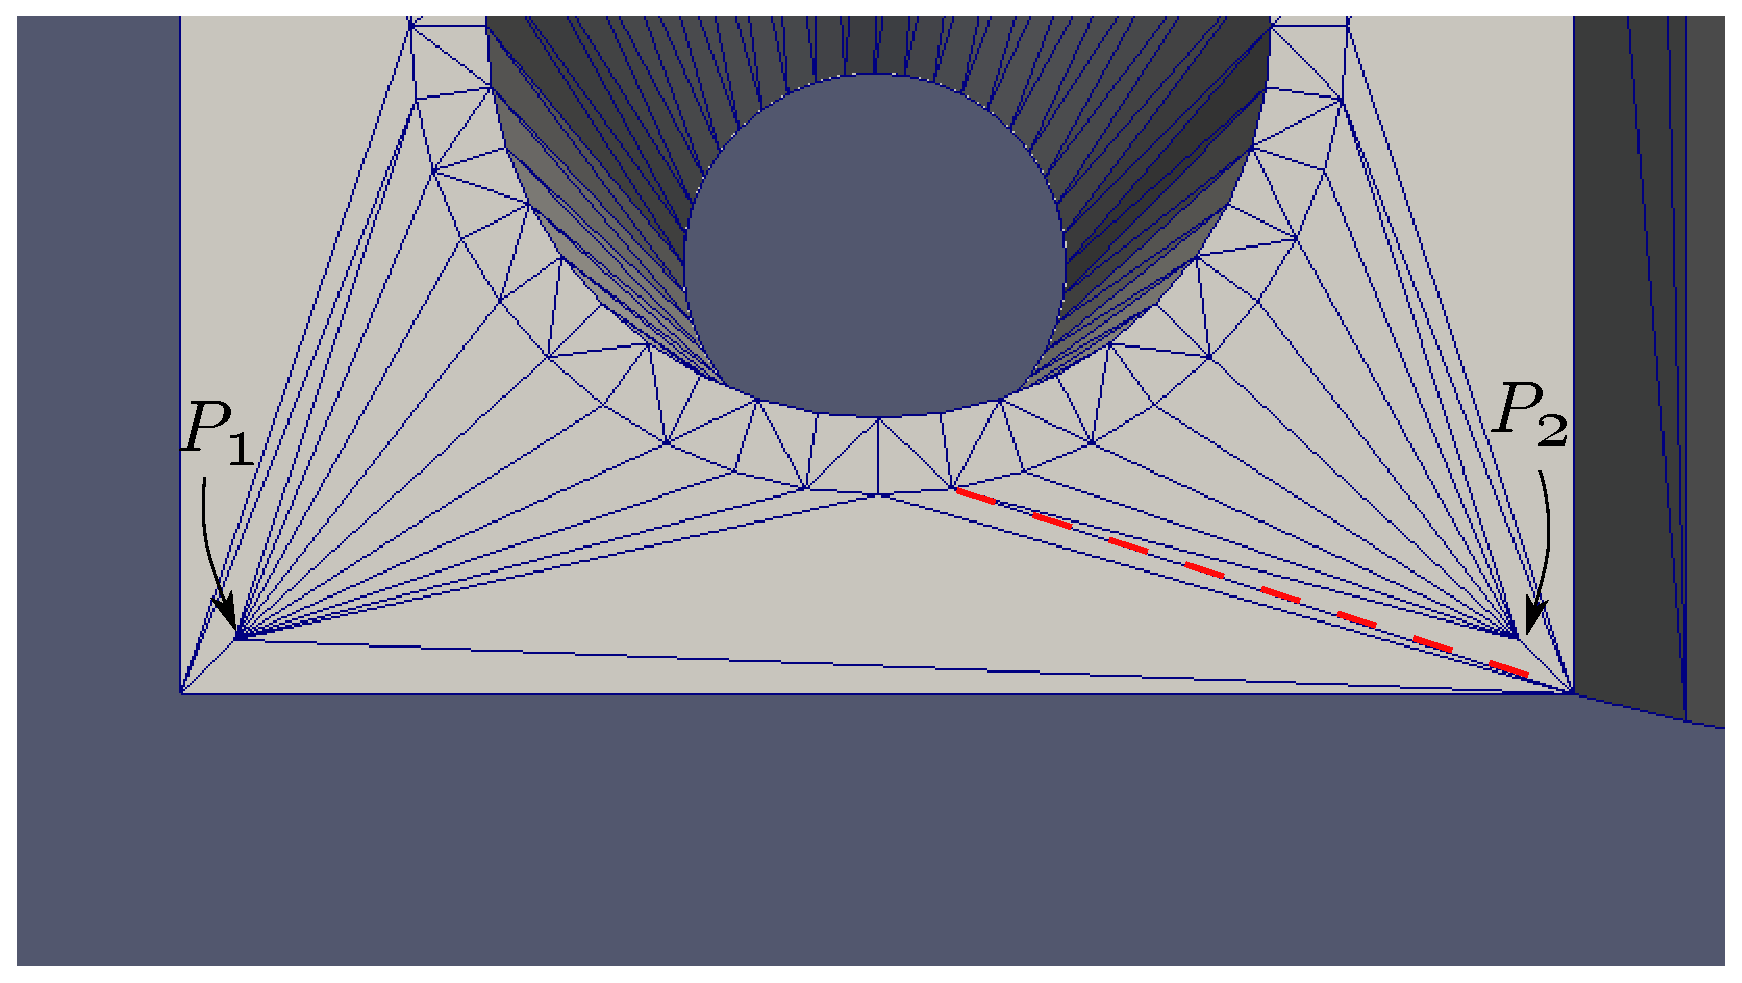
\includegraphics[width=.9\linewidth]{force-swapping-edge-recovery/swap2-edited.eps}
  \caption{}
  \label{force-swap3}
\end{subfigure}%
\begin{subfigure}{.5\textwidth}
  \centering
  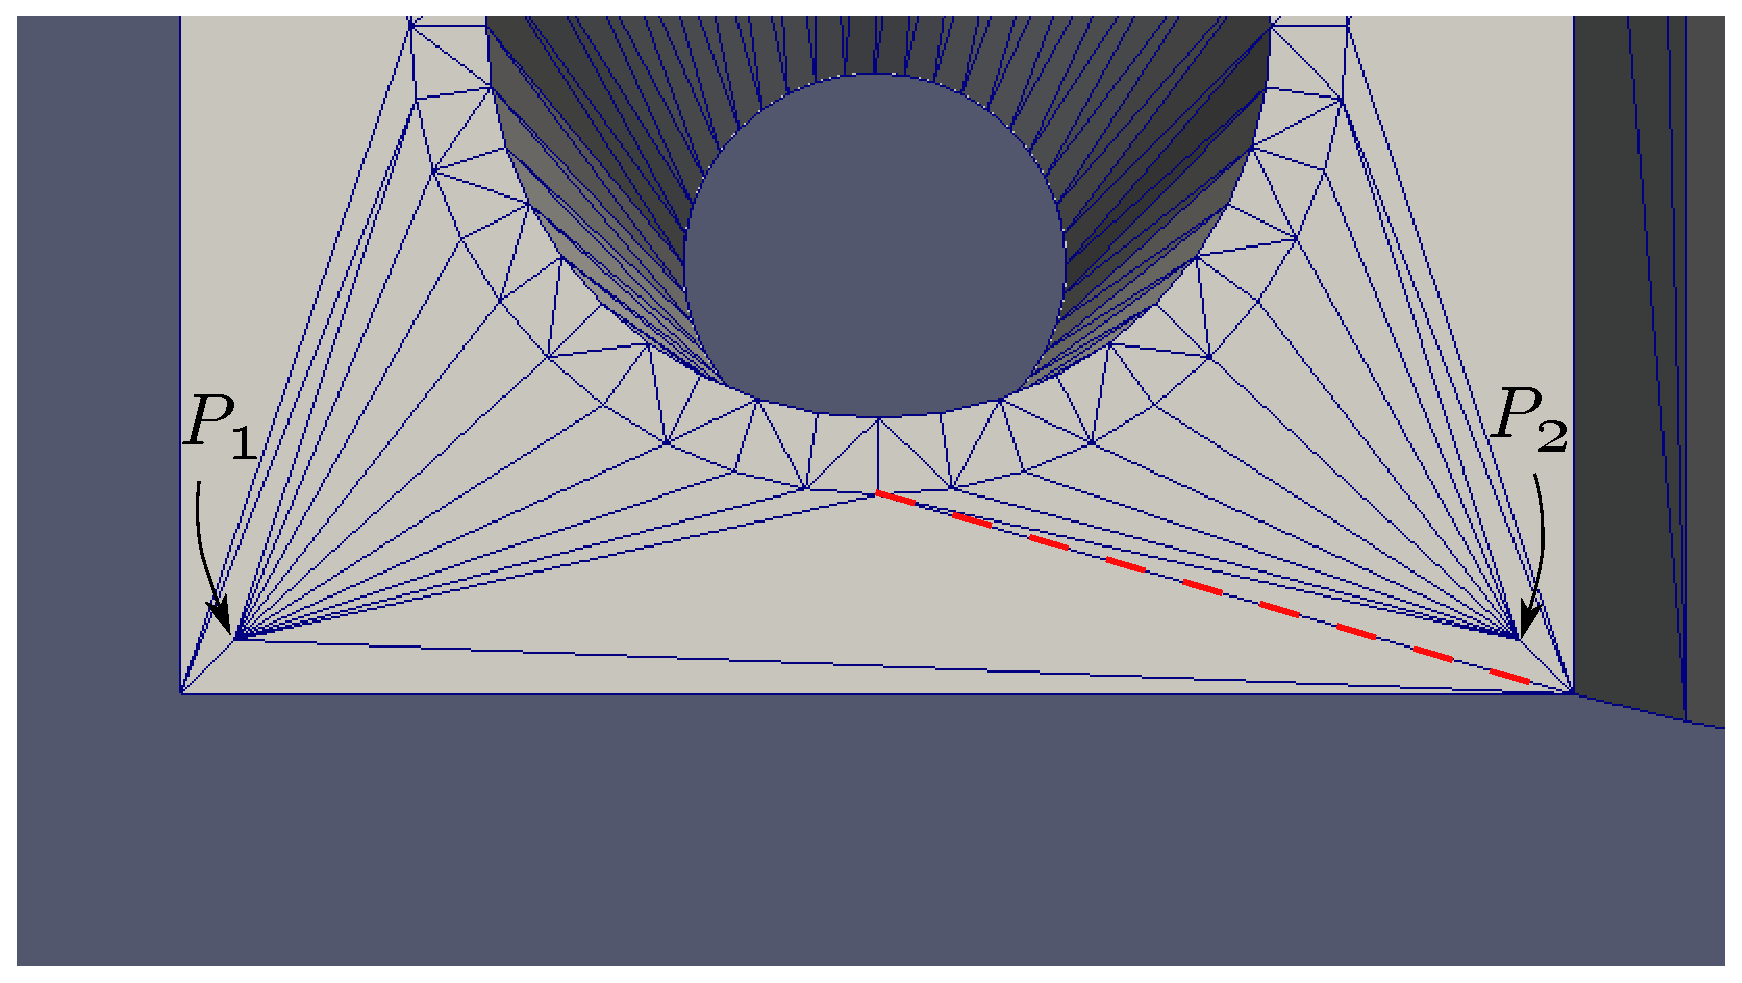
\includegraphics[width=.9\linewidth]{force-swapping-edge-recovery/swap3-edited.eps}
  \caption{}
  \label{force-swap4}
\end{subfigure}
\begin{subfigure}{.5\textwidth}
  \centering
  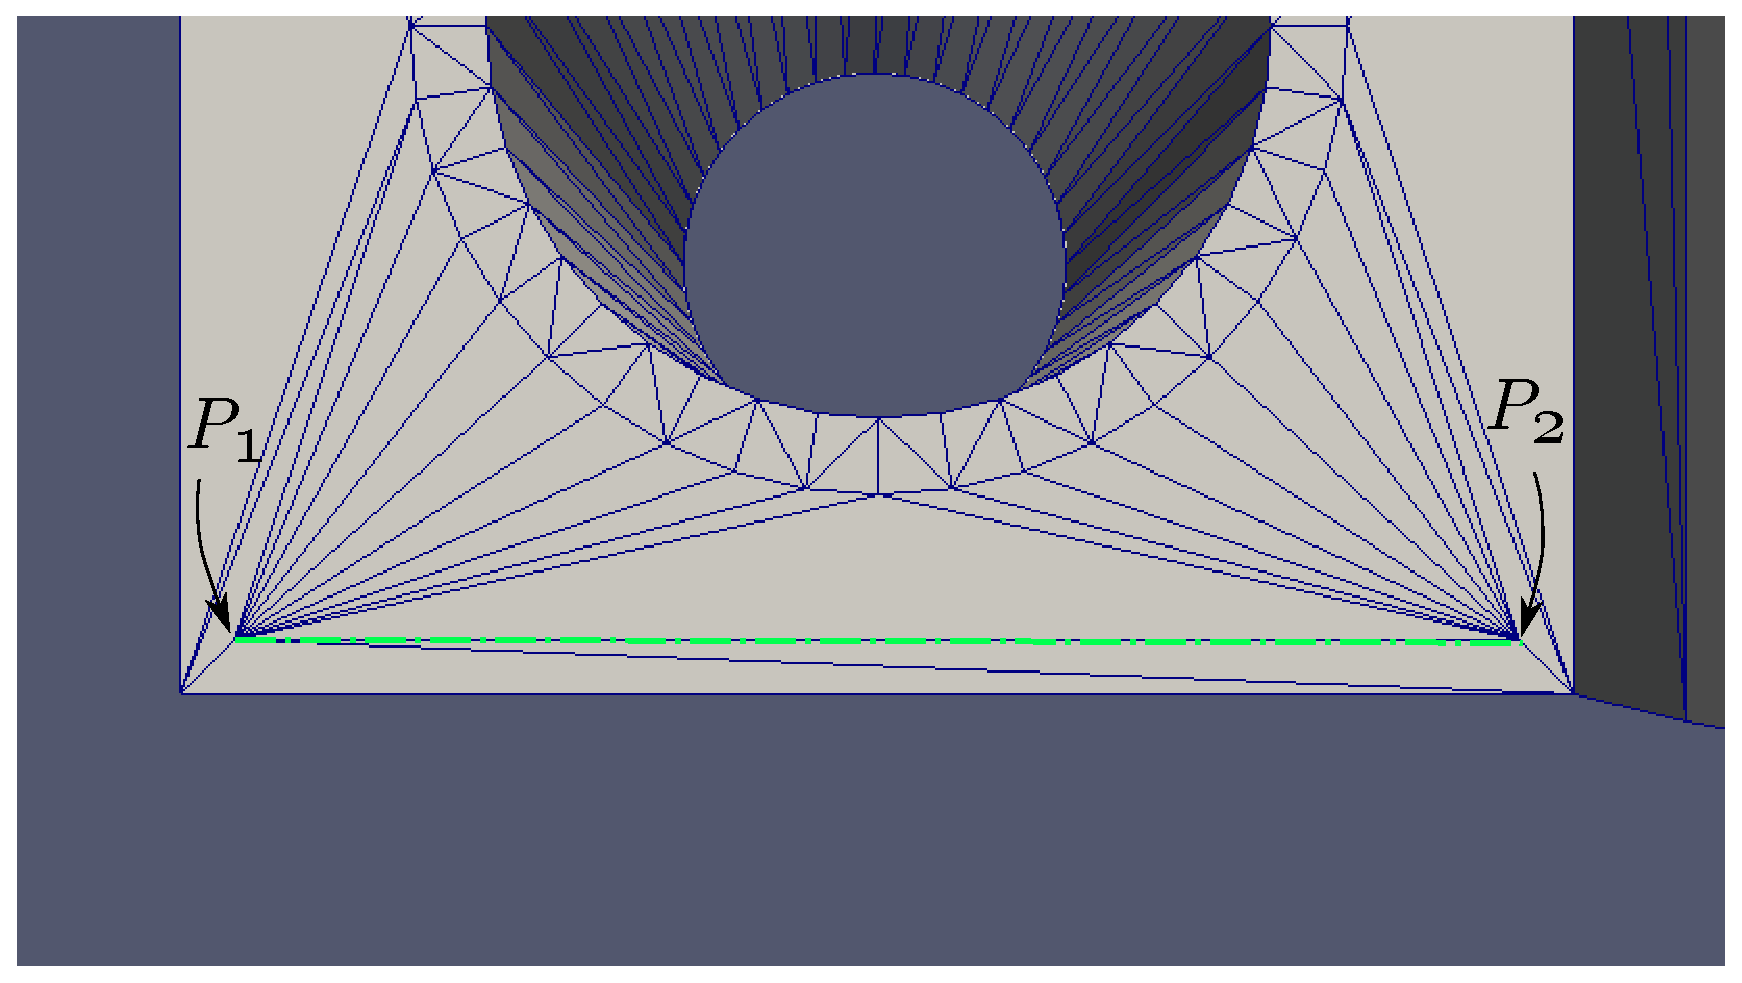
\includegraphics[width=.9\linewidth]{force-swapping-edge-recovery/swap4-edited.eps}
  \caption{}
  \label{force-swap5}
\end{subfigure}
\caption{Front Recovery: Point $P_1$ and point $P_2$ here represent the two kid points generated from the boundary of the surface. We try to force a connection between the two points by iteratively swapping edges which topologically obstruct their connection. Red dashed lines represents the edge chosen to be swapped next. In (e), the green edge is the edge recovered and would serve as a part of the next front in the mesh. Note that this example is for front recovery illustration purposes and the initial boundary discretization is too coarse to get a good-quality advancing layer mesh.}
\label{force-swap}
\end{figure}

Front recovery is done by selecting a pair of points from the parent layer and then forcing an edge between the points extruded from these parent points; that is by forcing an edge between the kid vertices in the extruded layer. An edge is forced between the kid vertices by iteratively swapping any edge that lies topologically between the two kid points. This kind of forced swapping in the mesh might seem to decrease mesh quality. However, with the right boundary discretization, it would help in giving us the high-aspect ratio elements in the mesh that we desire. After all the kid vertices are connected by this method, validation checks are run to ensure that the extruded layer is well defined and there are no discrepancies in this layer as it will serve as the parent layer for the next one. This incorporates checking the connectivity of each vertex with its adjacent edges and the connectivity of each edge with its end points. Figure \ref{force-swap} shows how exactly we recover an edge in the front by iteratively swapping the edges which obstruct the edge creation between two kid vertices, $P_1$ and $P_2$ in the figure. The edges which are topologically obstructing kid vertices $P_1$ and $P_2$ are swapped iteratively. A test is setup for each swap to avoid the flipping of triangles on the surface. After all the obstructing edges are swapped, a front edge between the kid vertices $P_1$ and $P_2$ would be recovered as shown in green in Figure \ref{force-swap5}.

\subsection{Edge Collapse and Interior Improvement}

As the advancing front moves into surface interior, we decimate interior vertices of the initial triangulation as well as boundary vertices which are too close to each other through edge-collapse.

Once we have recovered the advancing front by iterative edge swaps to connect the kid points in the mesh, we check for vertices on the front that are too close to each other relative to the extrusion length. For instance, vertices which are near a concave corner could encroach each other if they are not decimated. Another example would be vertices on the advancing front which are far away from surface boundaries because the extrusion length has grown by this point. Decimating vertices from the front which are at a substantial distance from surface boundaries helps prevent the cell aspect ratio, ie front edge length over extrusion length from dropping below one.

To check for vertices to decimate, we iterate through the vertices in the front and identify the ones which are too close to their neighbours. Vertex decimation is done through the edge-collapse routine as described in \cite{hoppe1994mesh}. The threshold edge length between two points on the front is set to be $2 tan(\pi/8)$ times the average extrusion length at those points. This value is set so as to minimize the normalized maximum deviation of angle from $90$ degree for quad elements. Hence, the threshold ensures that the anisotropic properties are retained for several layers into the surface. All short edges on the front are collapsed using the edge-collapse algorithm. An example of an edge-collapse on the front is shown in Figure \ref{edge-collapse}. Here, two points $P_1$ and $P_2$ are collapsed into a single point which forms a part of the next front on the surface.

As the advancing front marches into the surface, vertices in the interior of the surface immediately next to the front are decimated to make way for the advancing layers. Before extruding a point on the advancing front, we check if any point in the surface interior with which it shares an edge agrees with the following condition. If it does, we decimate the interior vertex.

\begin{equation}
    d < max(l_{1}/\sqrt{2}, l_{2}/\sqrt{2}, c\times extrudeLength)
    \label{collapse-eq}
\end{equation}

Here $d$ is the distance between the point on the advancing front and the interior point, $l_1$ and $l_2$ are the lengths of adjacent edges of the point on the front, c is a constant whose value is set as $2$ and $extrudeLength$ is the extrusion length at the vertex on the front. This condition ensures decimation of vertices in surface interior which are close to the advancing front and avoids any encroachment of surface interior vertices on the advancing layers. Topological and geometrical checks are done before an edge can be collapsed. These include a threshold for the ratio of area of generated triangles and a limit on the dihedral angle between the adjacent triangles created by the collapse. The area threshold is set to be $10^8$. Also, edge-collapse is successful only if the triangles resulting from it are be within a limit of $\theta < \ang{30}$ from the surface(see Figure \ref{deviation-surface}). The threshold for the maximum dihedral angle between any two adjacent triangles that result from the edge-collapse is set to $\ang{40}$. The quality criterion used for edge collapse is again maximization of the minimum angle in the triangles thus produced. The best edge for collapse is chosen when decimating the interior vertices using this quality criterion. This is in contrast to the vertex decimation on the advancing front where the candidate edge for collapse is already identified. An illustrative example for surface interior vertex decimation can be seen in Figure \ref{interior-vert-collapse}.

\begin{figure}[hbt!]
\centering
\begin{subfigure}{.5\textwidth}
  \centering
  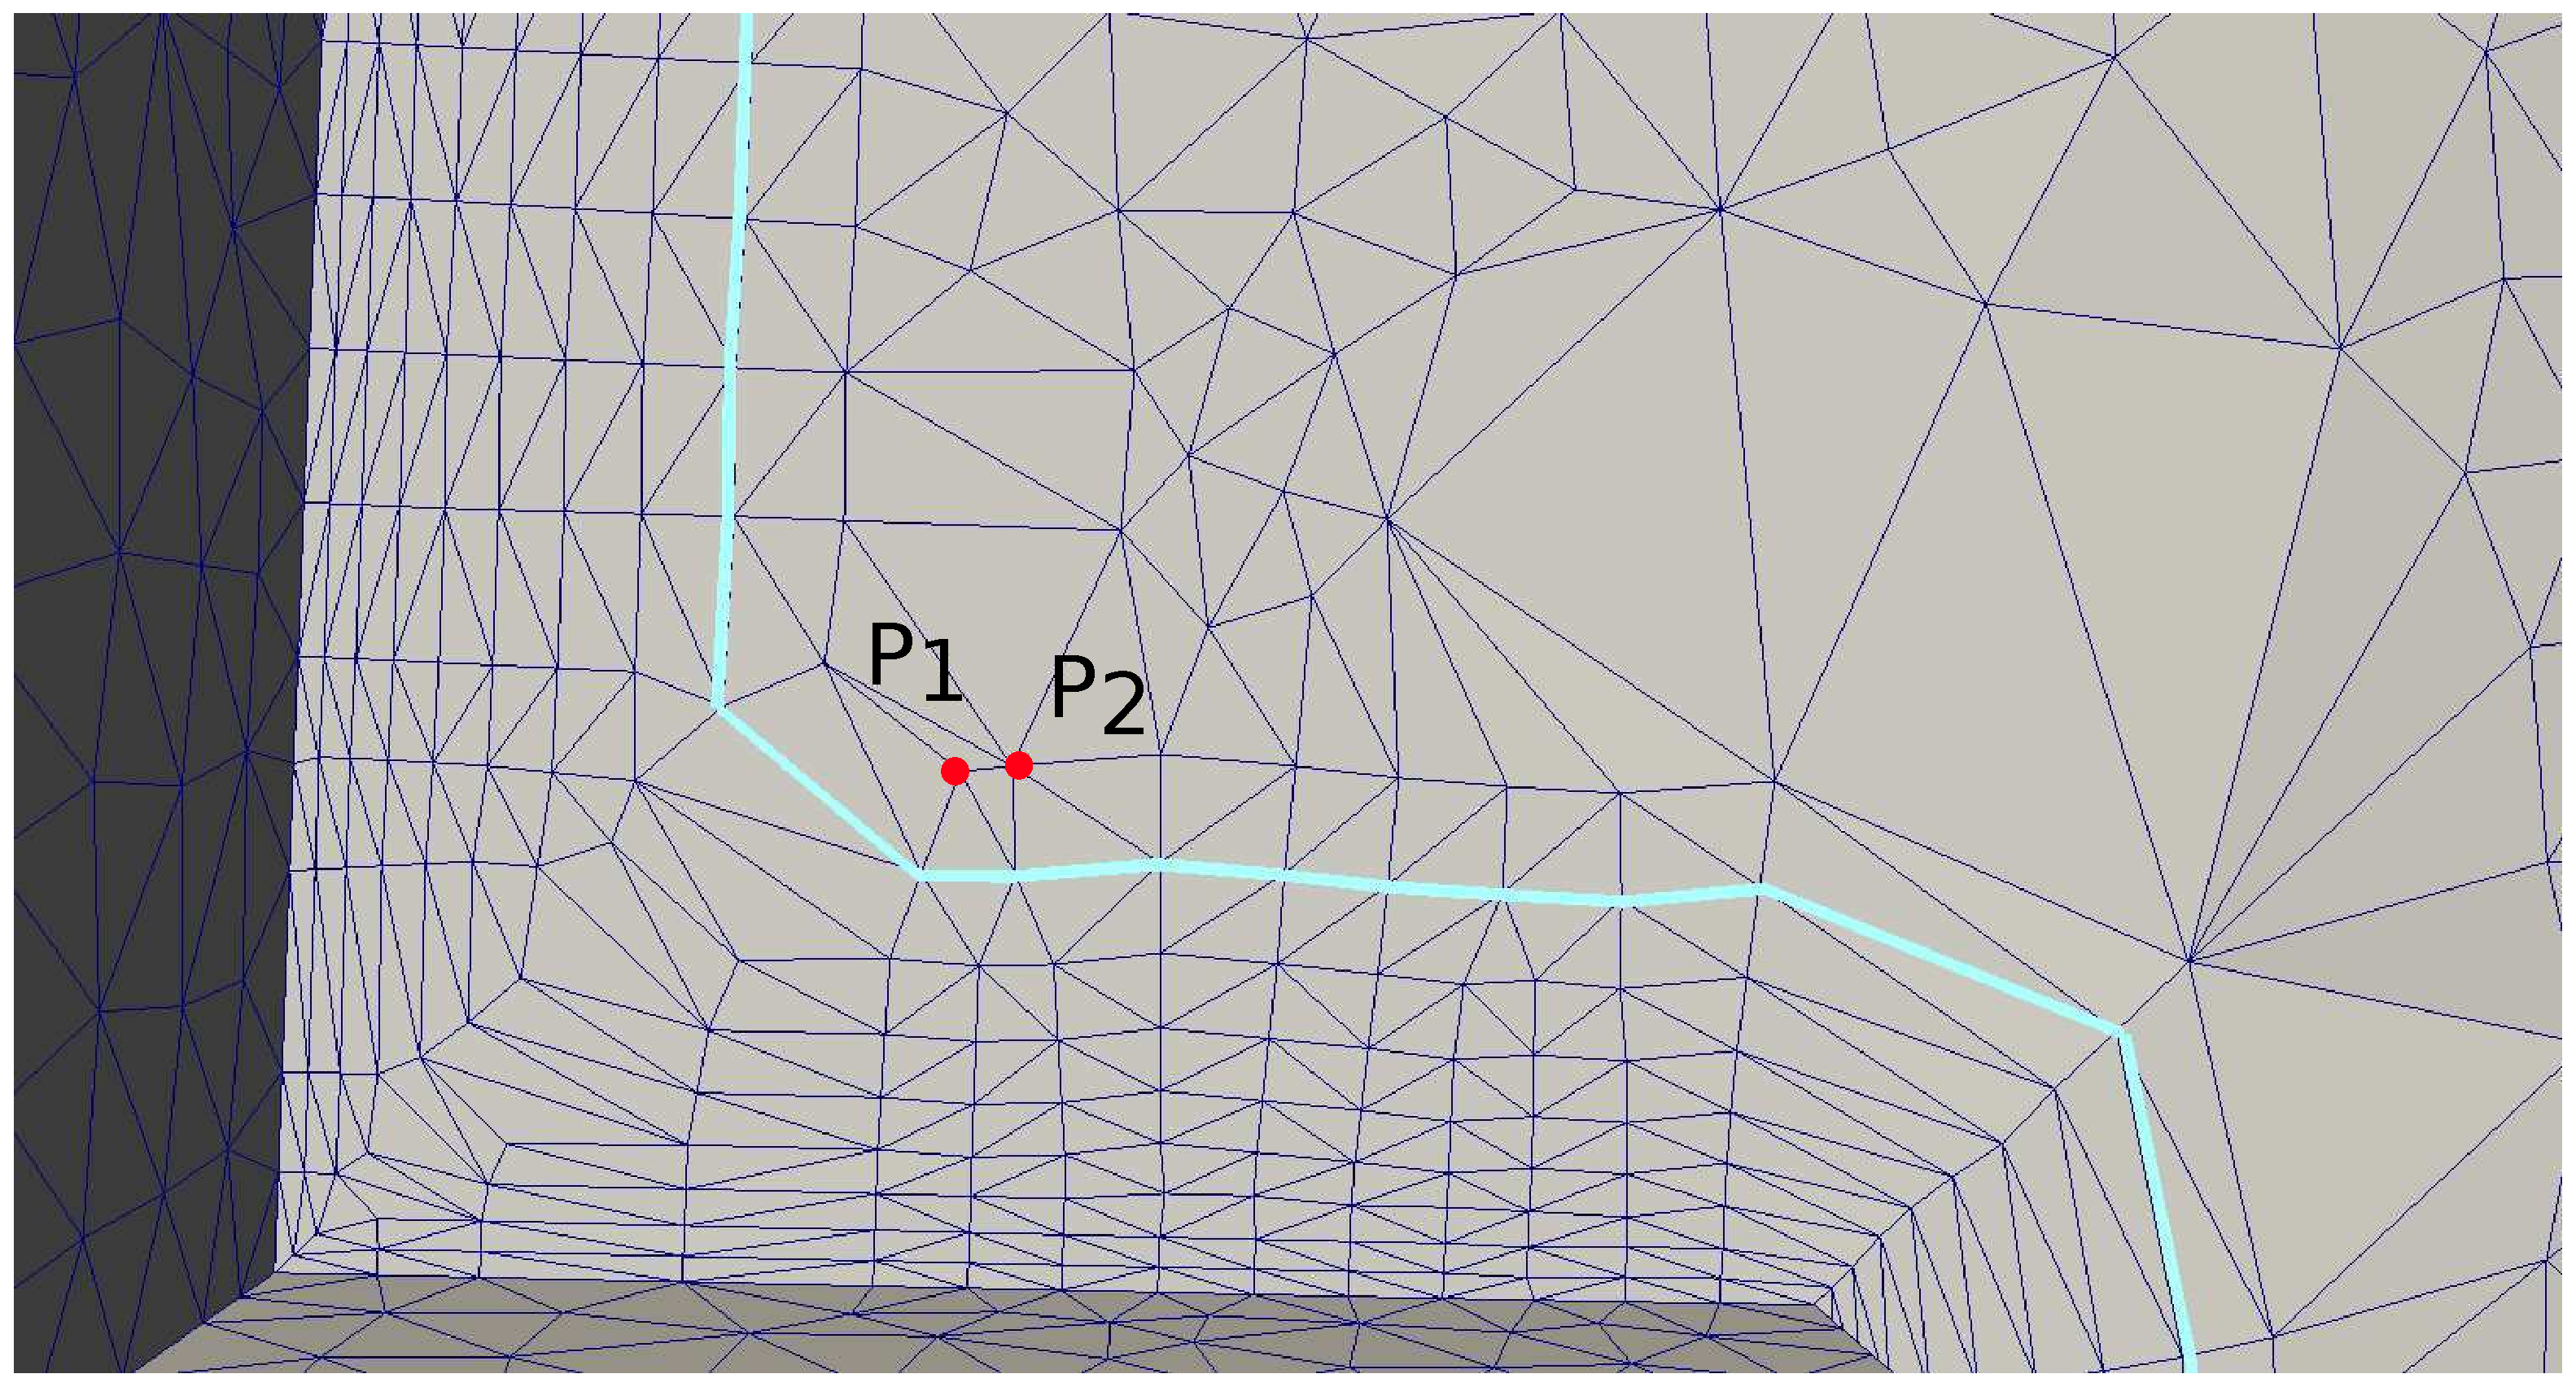
\includegraphics[width=.9\linewidth]{edge-collapse/collapse1.eps}
  \caption{}
  \label{collapse1}
\end{subfigure}%
\begin{subfigure}{.5\textwidth}
  \centering
  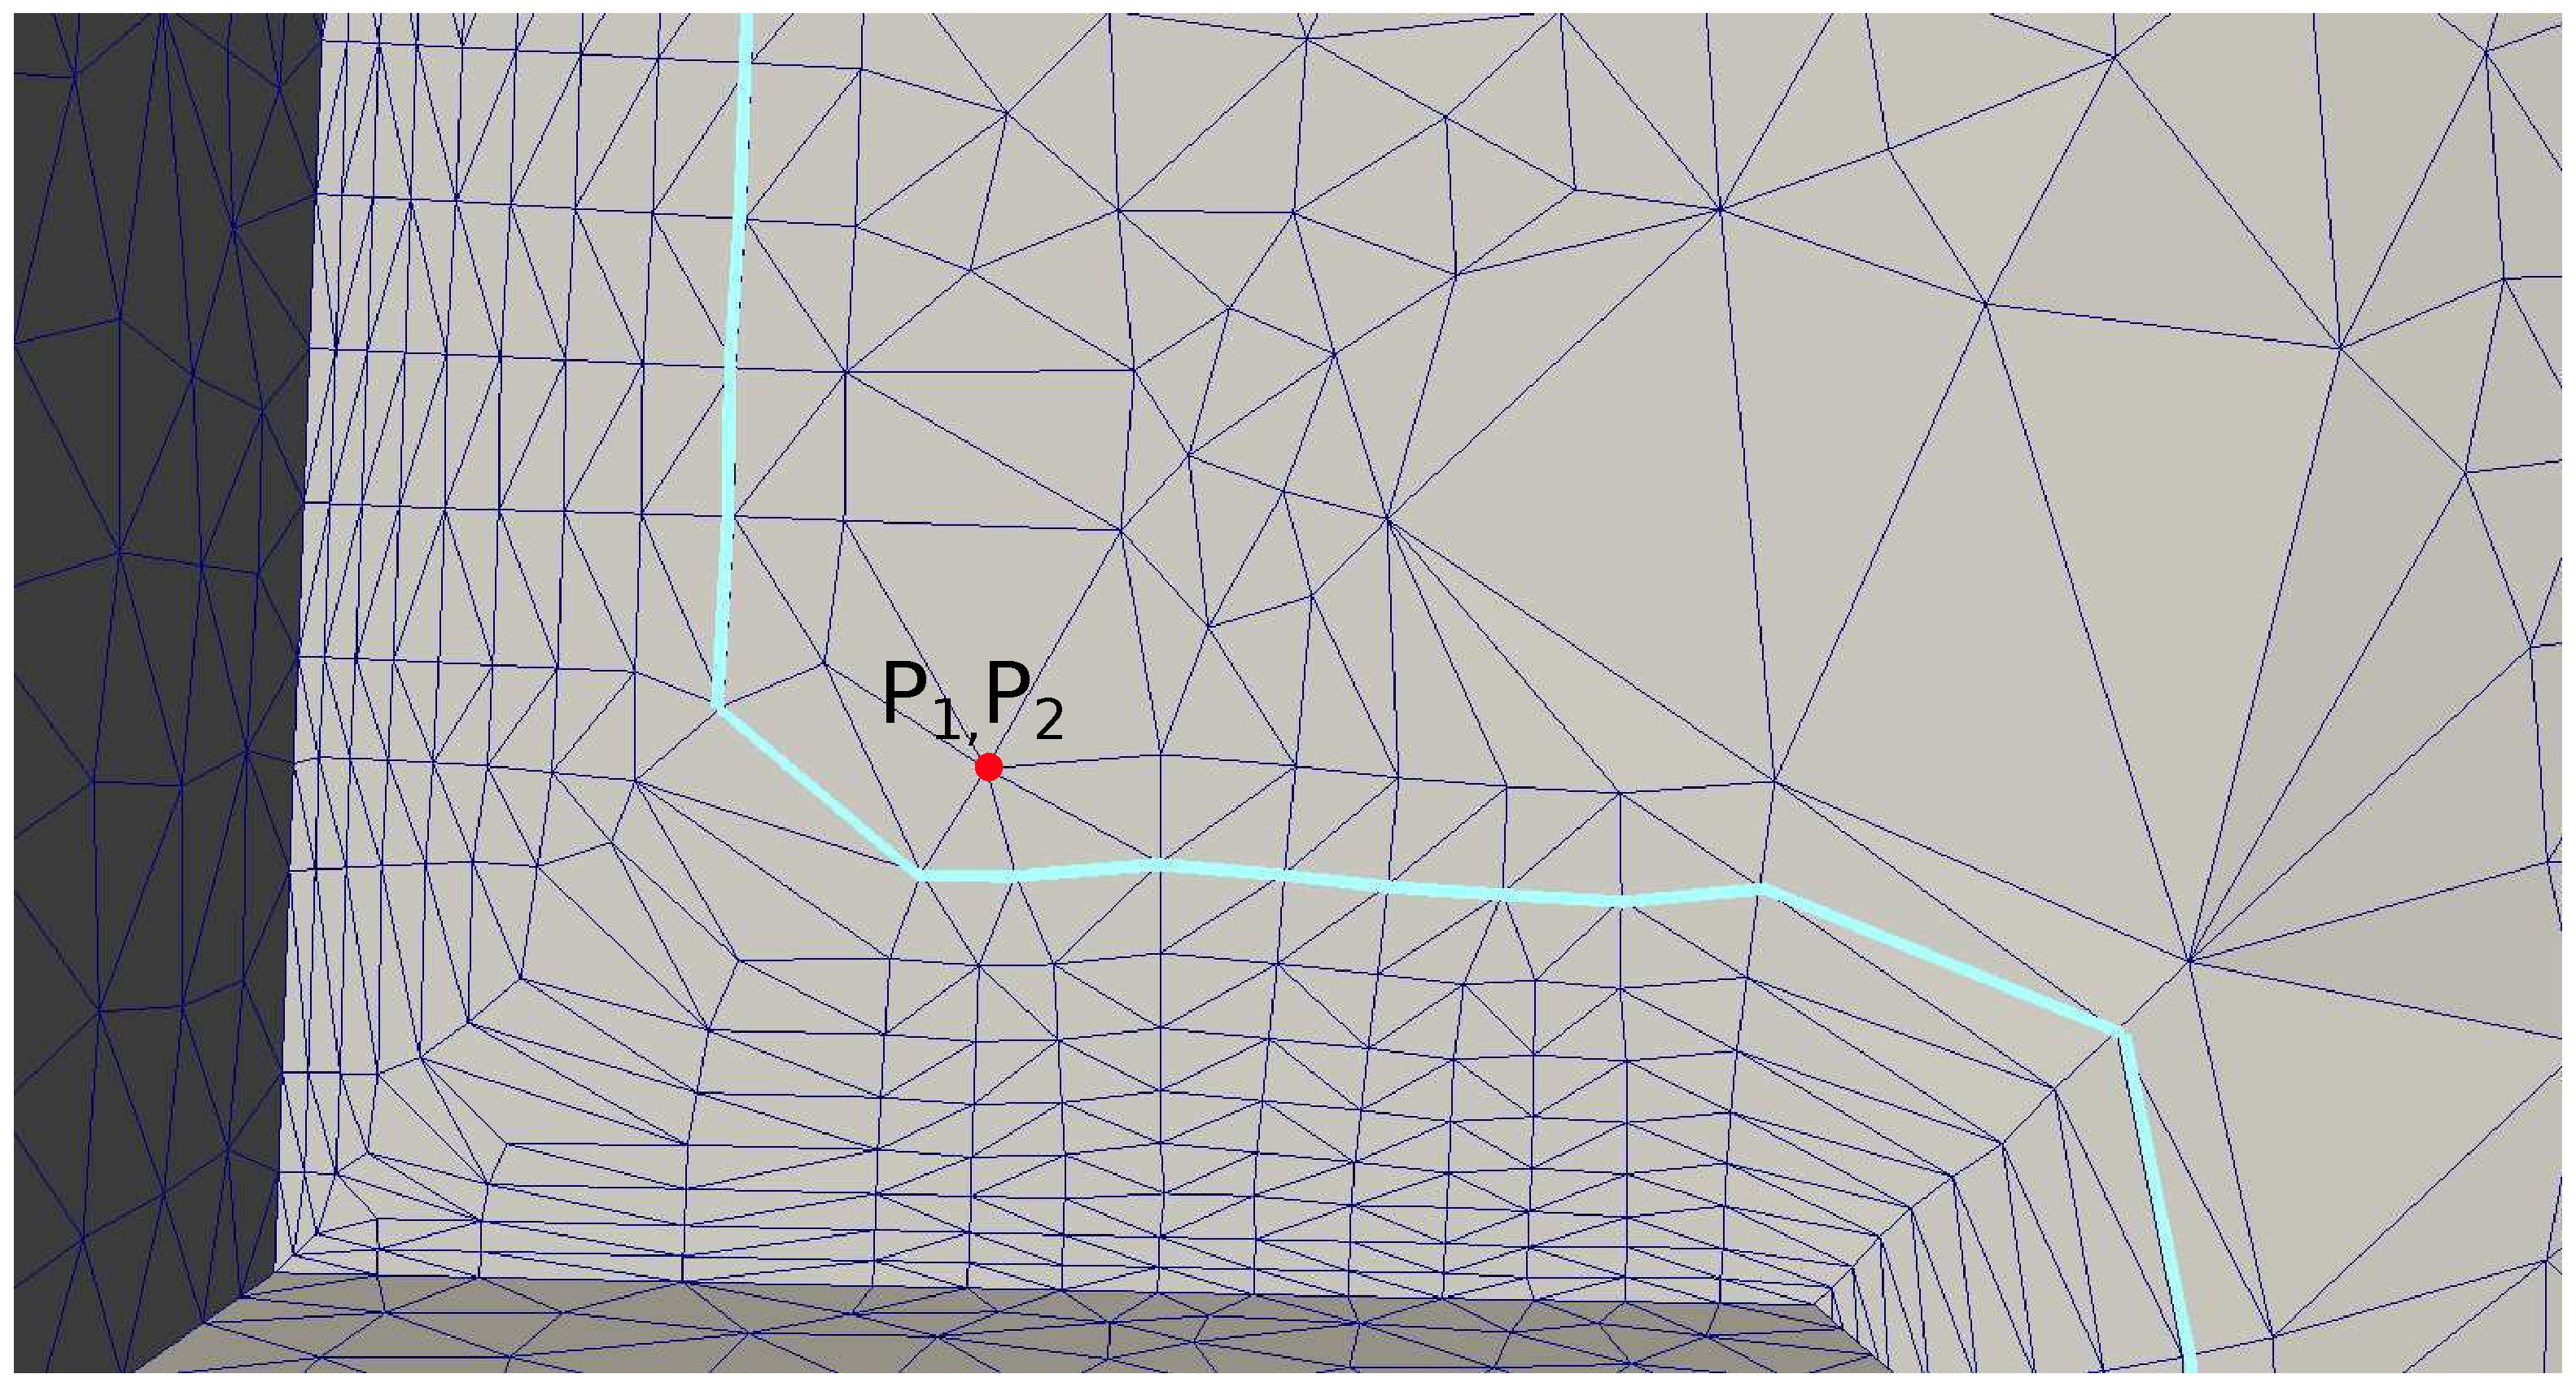
\includegraphics[width=.9\linewidth]{edge-collapse/collapse2.eps}
  \caption{}
  \label{collapse2}
\end{subfigure}
\begin{subfigure}{.5\textwidth}
  \centering
  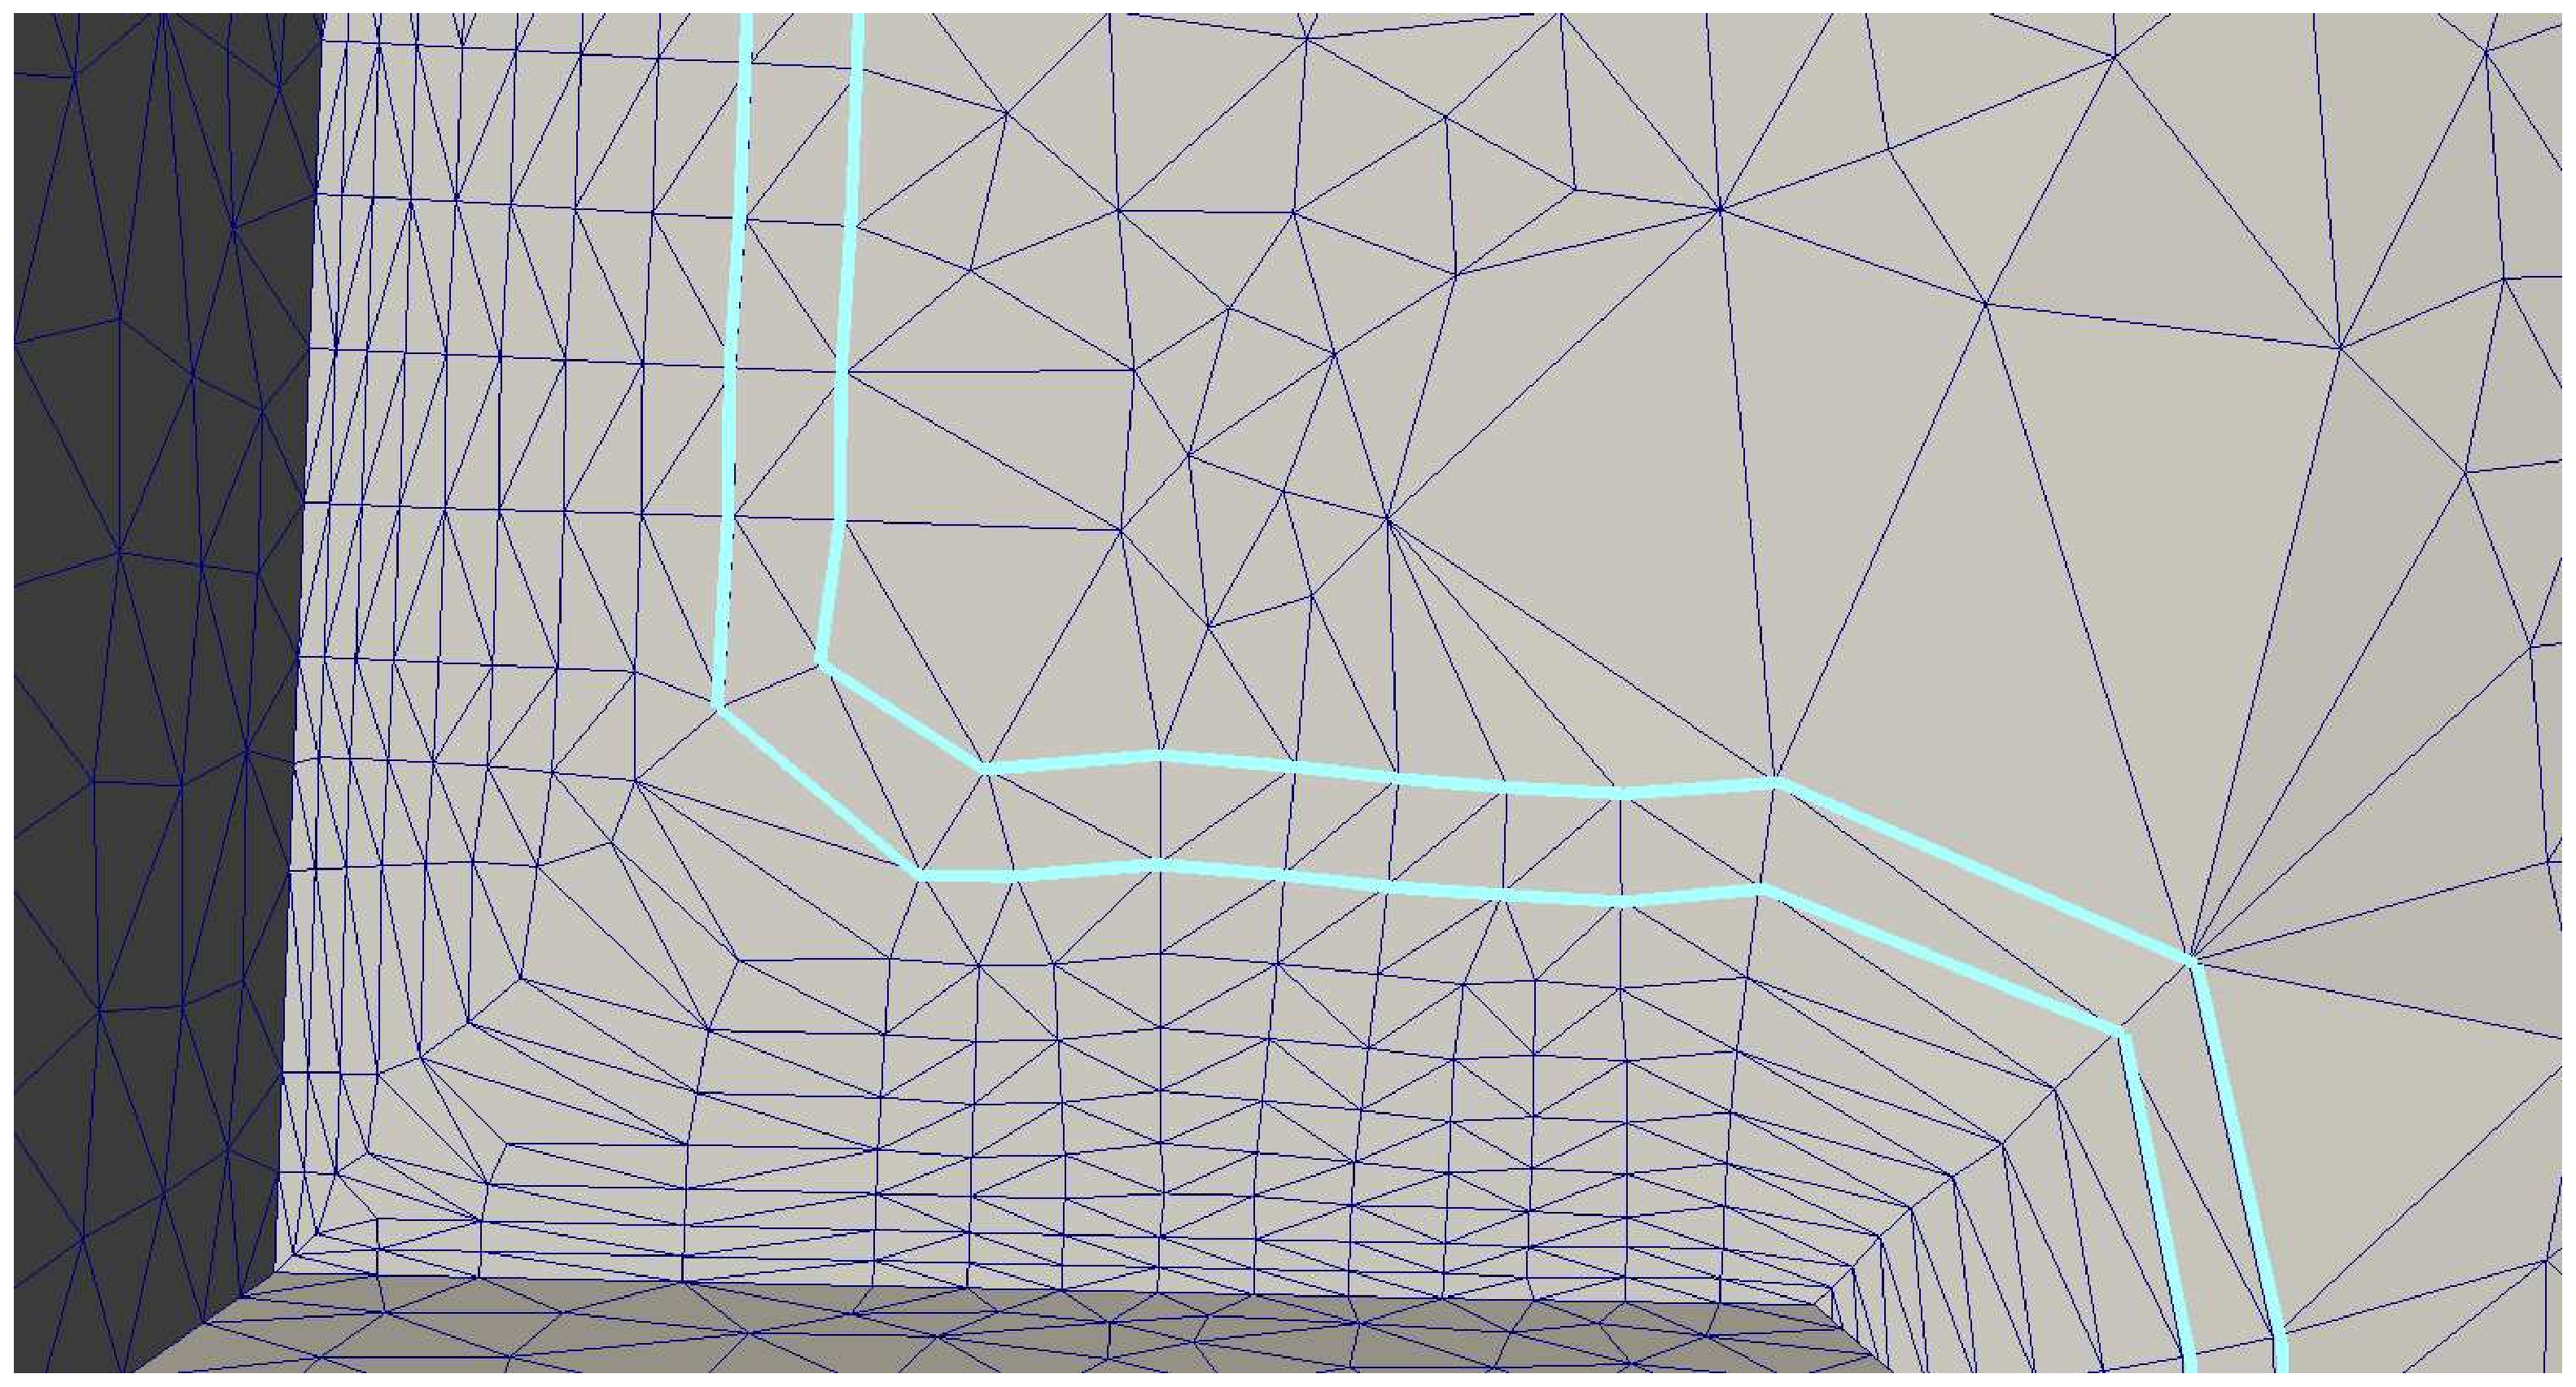
\includegraphics[width=.9\linewidth]{edge-collapse/collapse3.eps}
  \caption{}
  \label{collapse3}
\end{subfigure}
\caption{Edge collapse on an advancing front to avoid encroachment of points. In (a), two points in the kid layer $P_1$ and $P_2$ are sufficiently close to each other. Their parent layer is highlighted. If both the points advance to the next layer, then the next front would fail to recover. Hence, the edge between them is chosen to collapse. (b) shows the result of the edge collapse. The new location of both the points is the average position of their initial location. (c) shows how the next front looks like.}
\label{edge-collapse}
\end{figure}

After we have a recovered the front and decimated encroaching vertices in the surface interior as well as on the advancing front through edge collapse, we queue up the immediate interior edges of the surface and swap them for maximizing mesh quality. This step is included so that we have a good interior triangulation at each step of the advancing layer routine. This step ensures that we do not have bad triangles causing problems as we continue to march.

\begin{figure}[hbt!]
\centering
\begin{subfigure}{.5\textwidth}
  \centering
  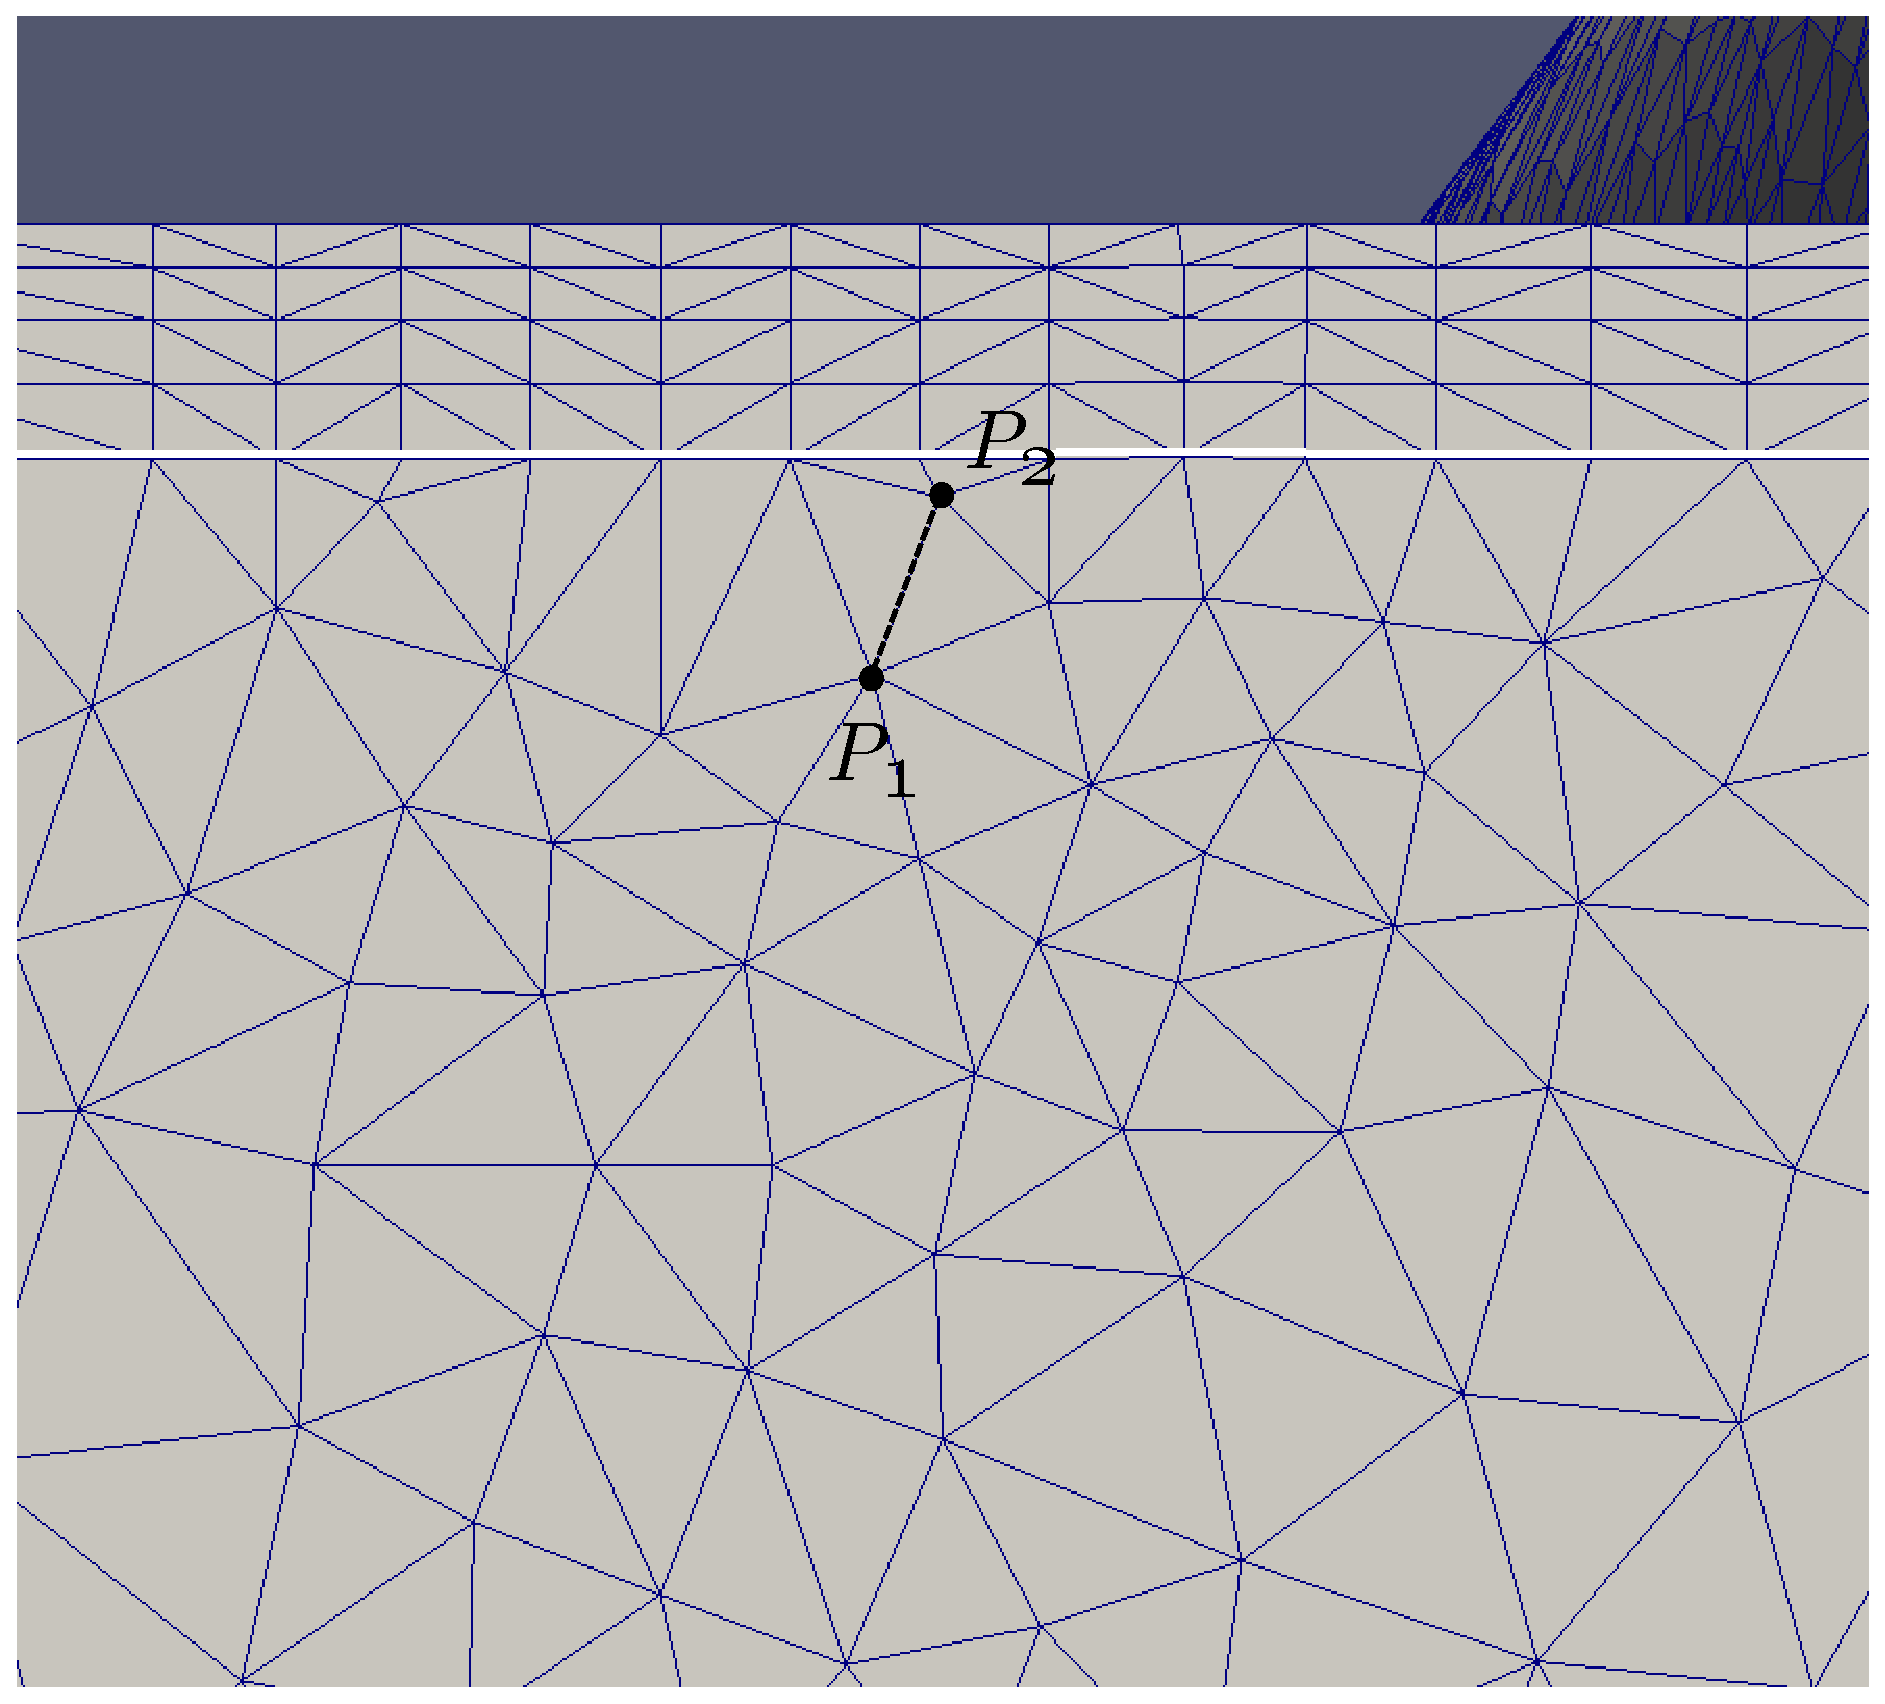
\includegraphics[width=.9\linewidth]{interior-vert-collapse/cc1.eps}
  \caption{}
  \label{cc1}
\end{subfigure}%
\begin{subfigure}{.5\textwidth}
  \centering
  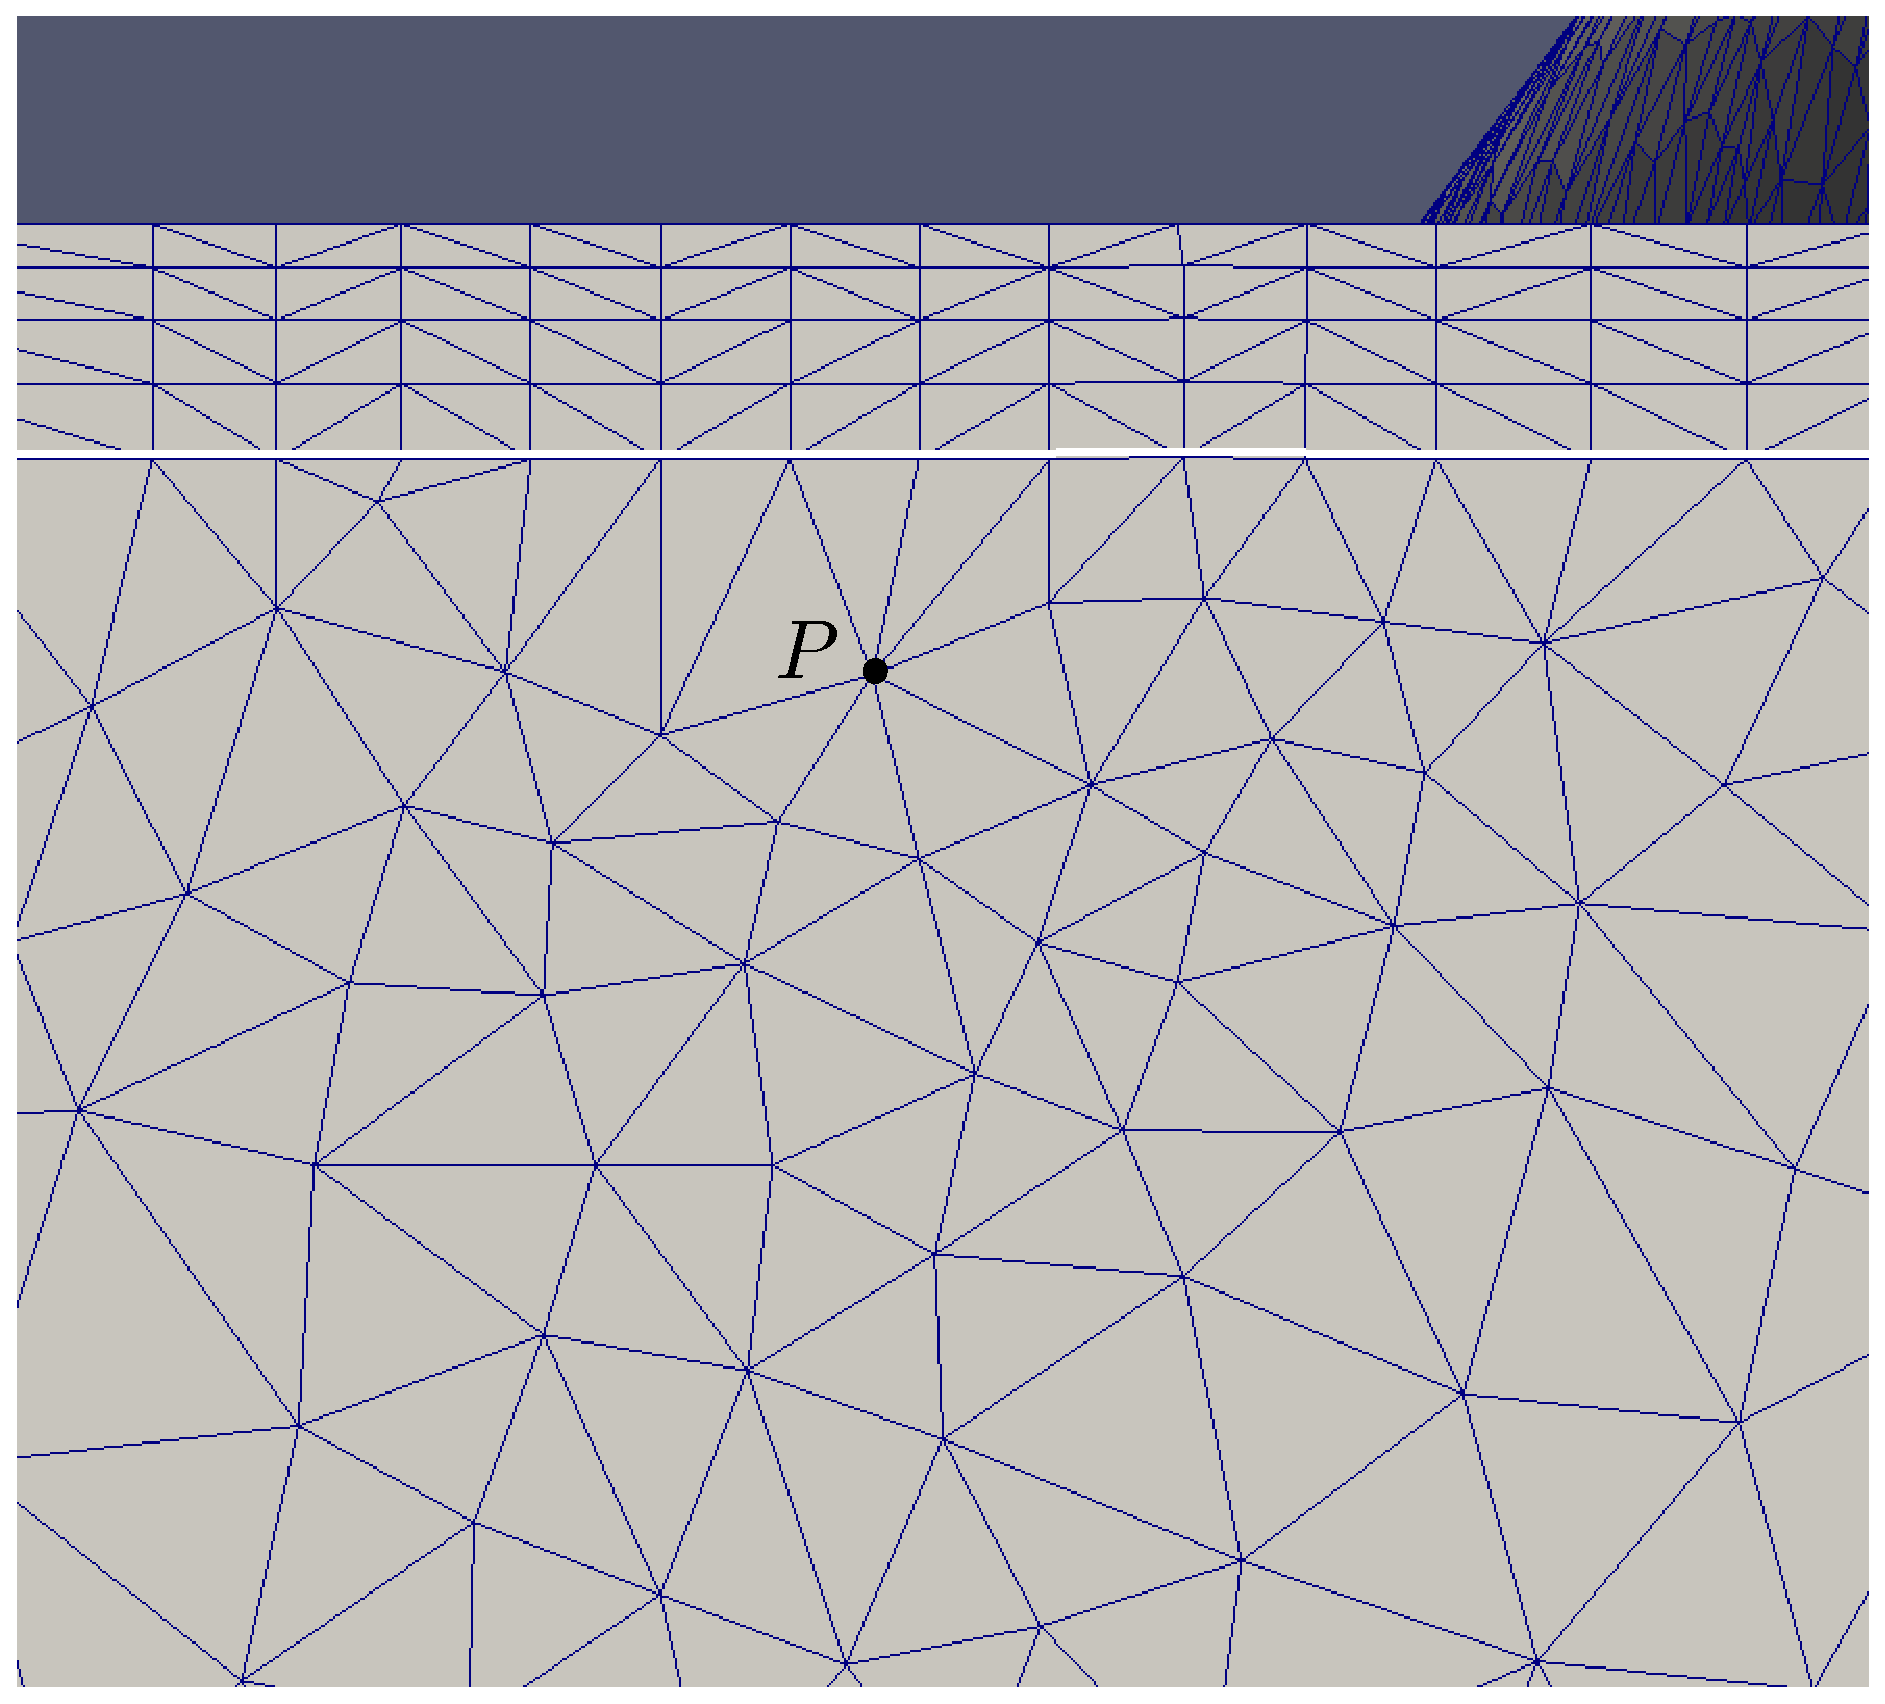
\includegraphics[width=.9\linewidth]{interior-vert-collapse/cc2.eps}
  \caption{}
  \label{cc2}
\end{subfigure}
\begin{subfigure}{.5\textwidth}
  \centering
  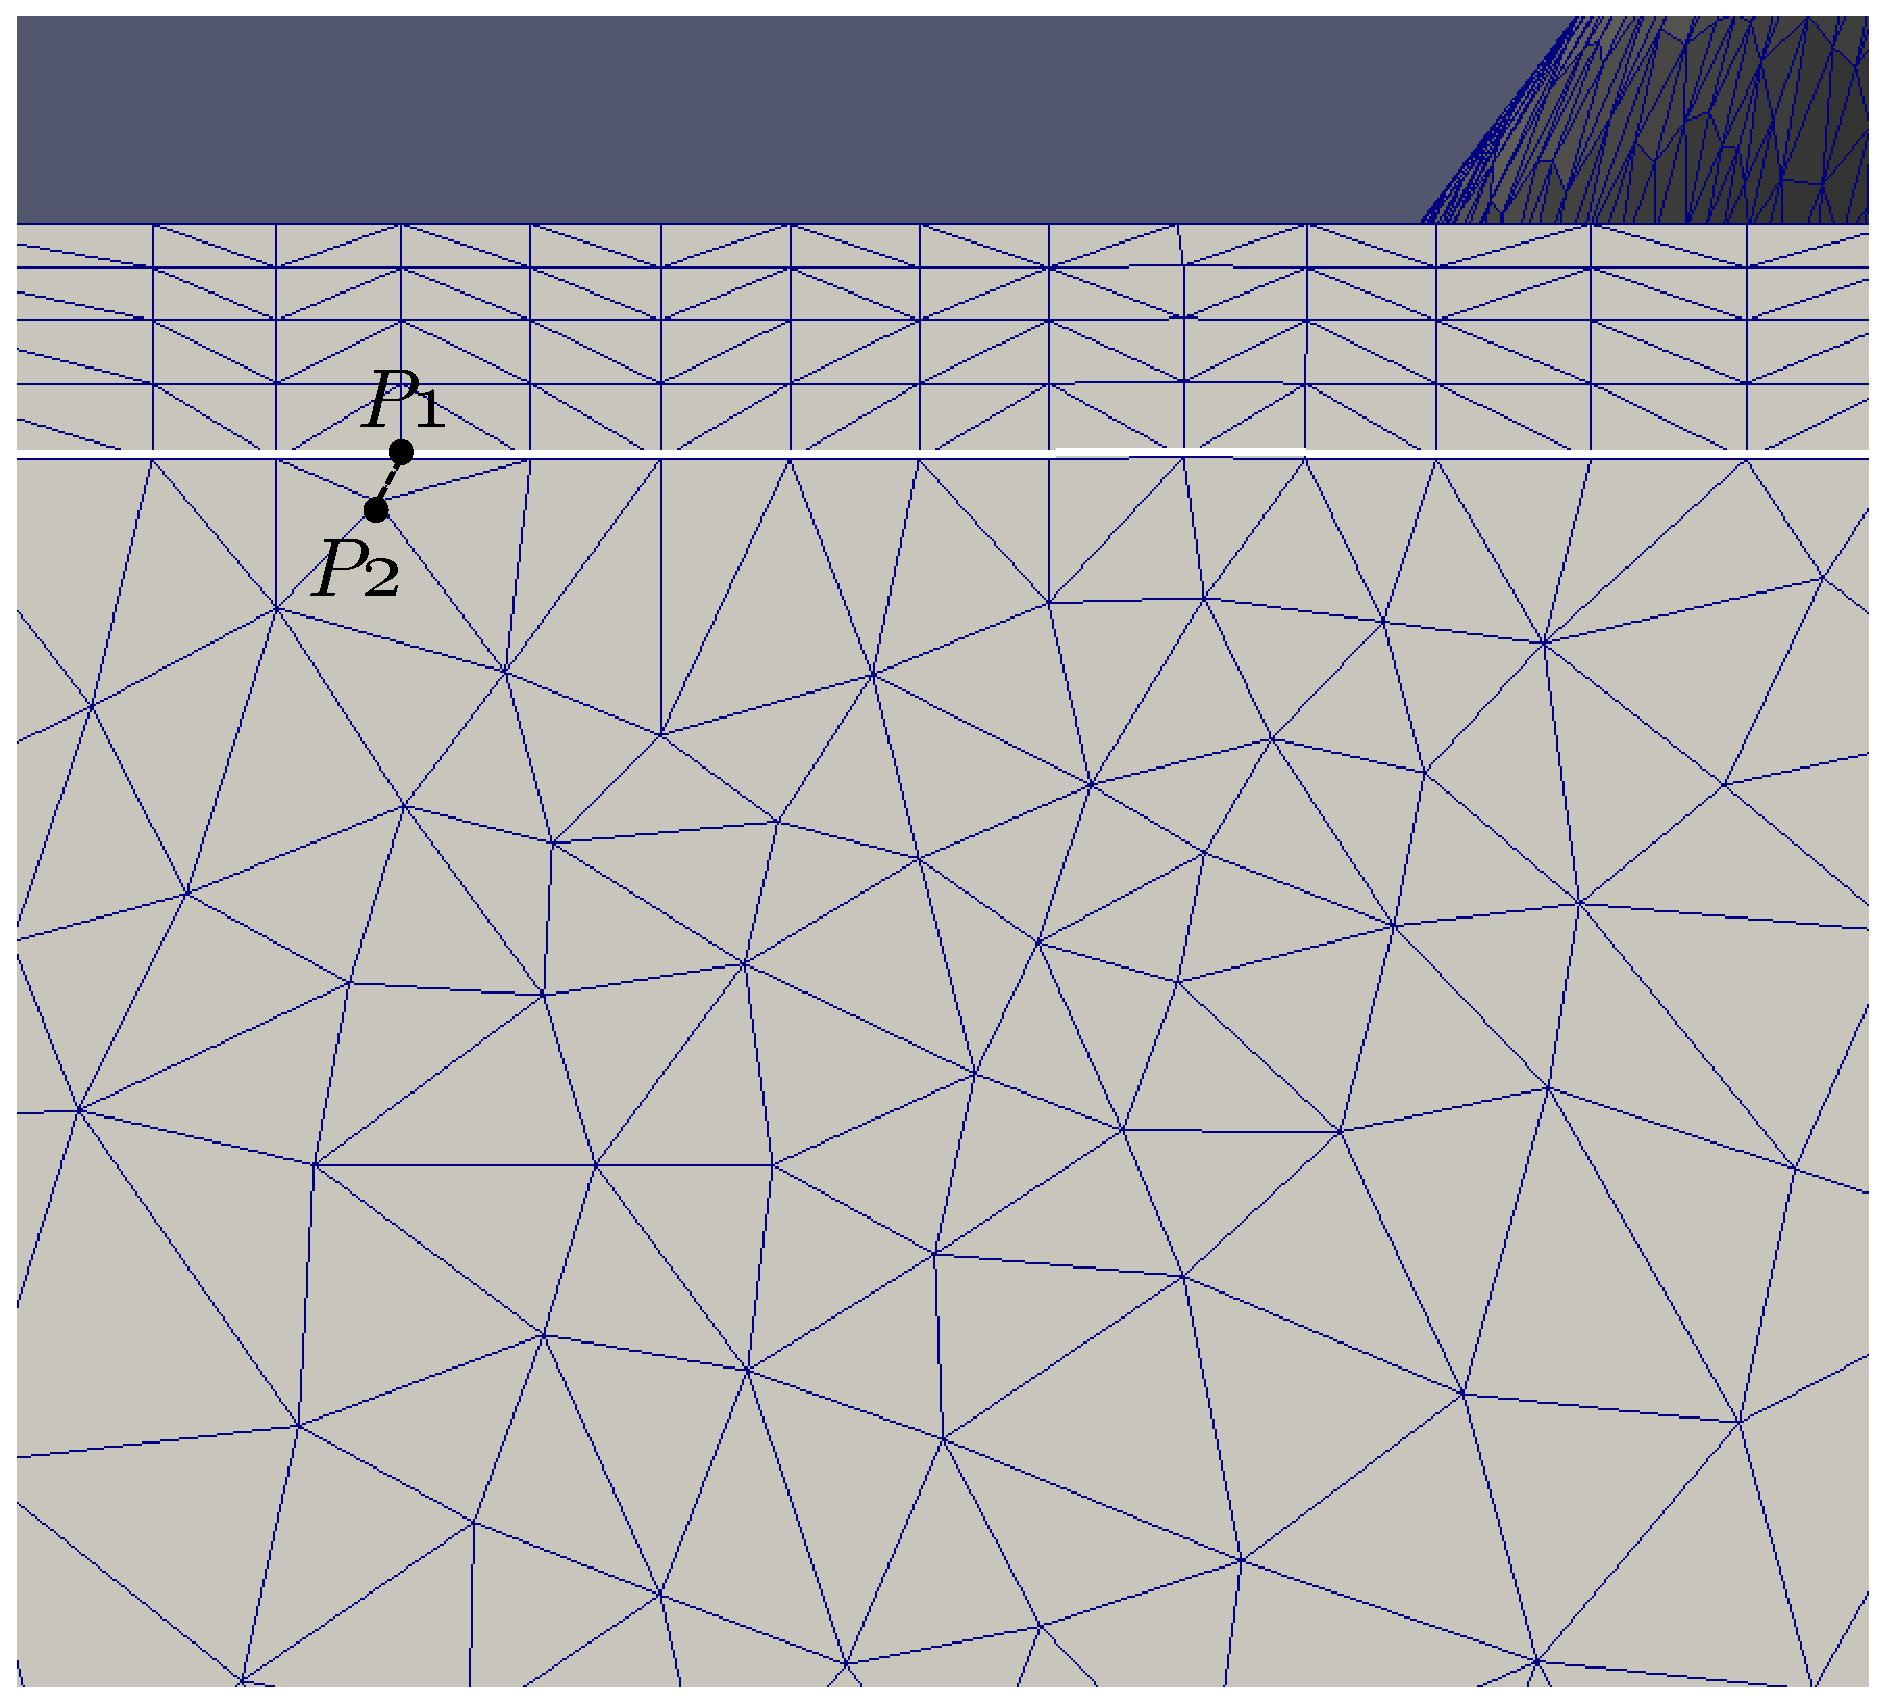
\includegraphics[width=.9\linewidth]{interior-vert-collapse/cc3.eps}
  \caption{}
  \label{cc3}
\end{subfigure}%
\begin{subfigure}{.5\textwidth}
  \centering
  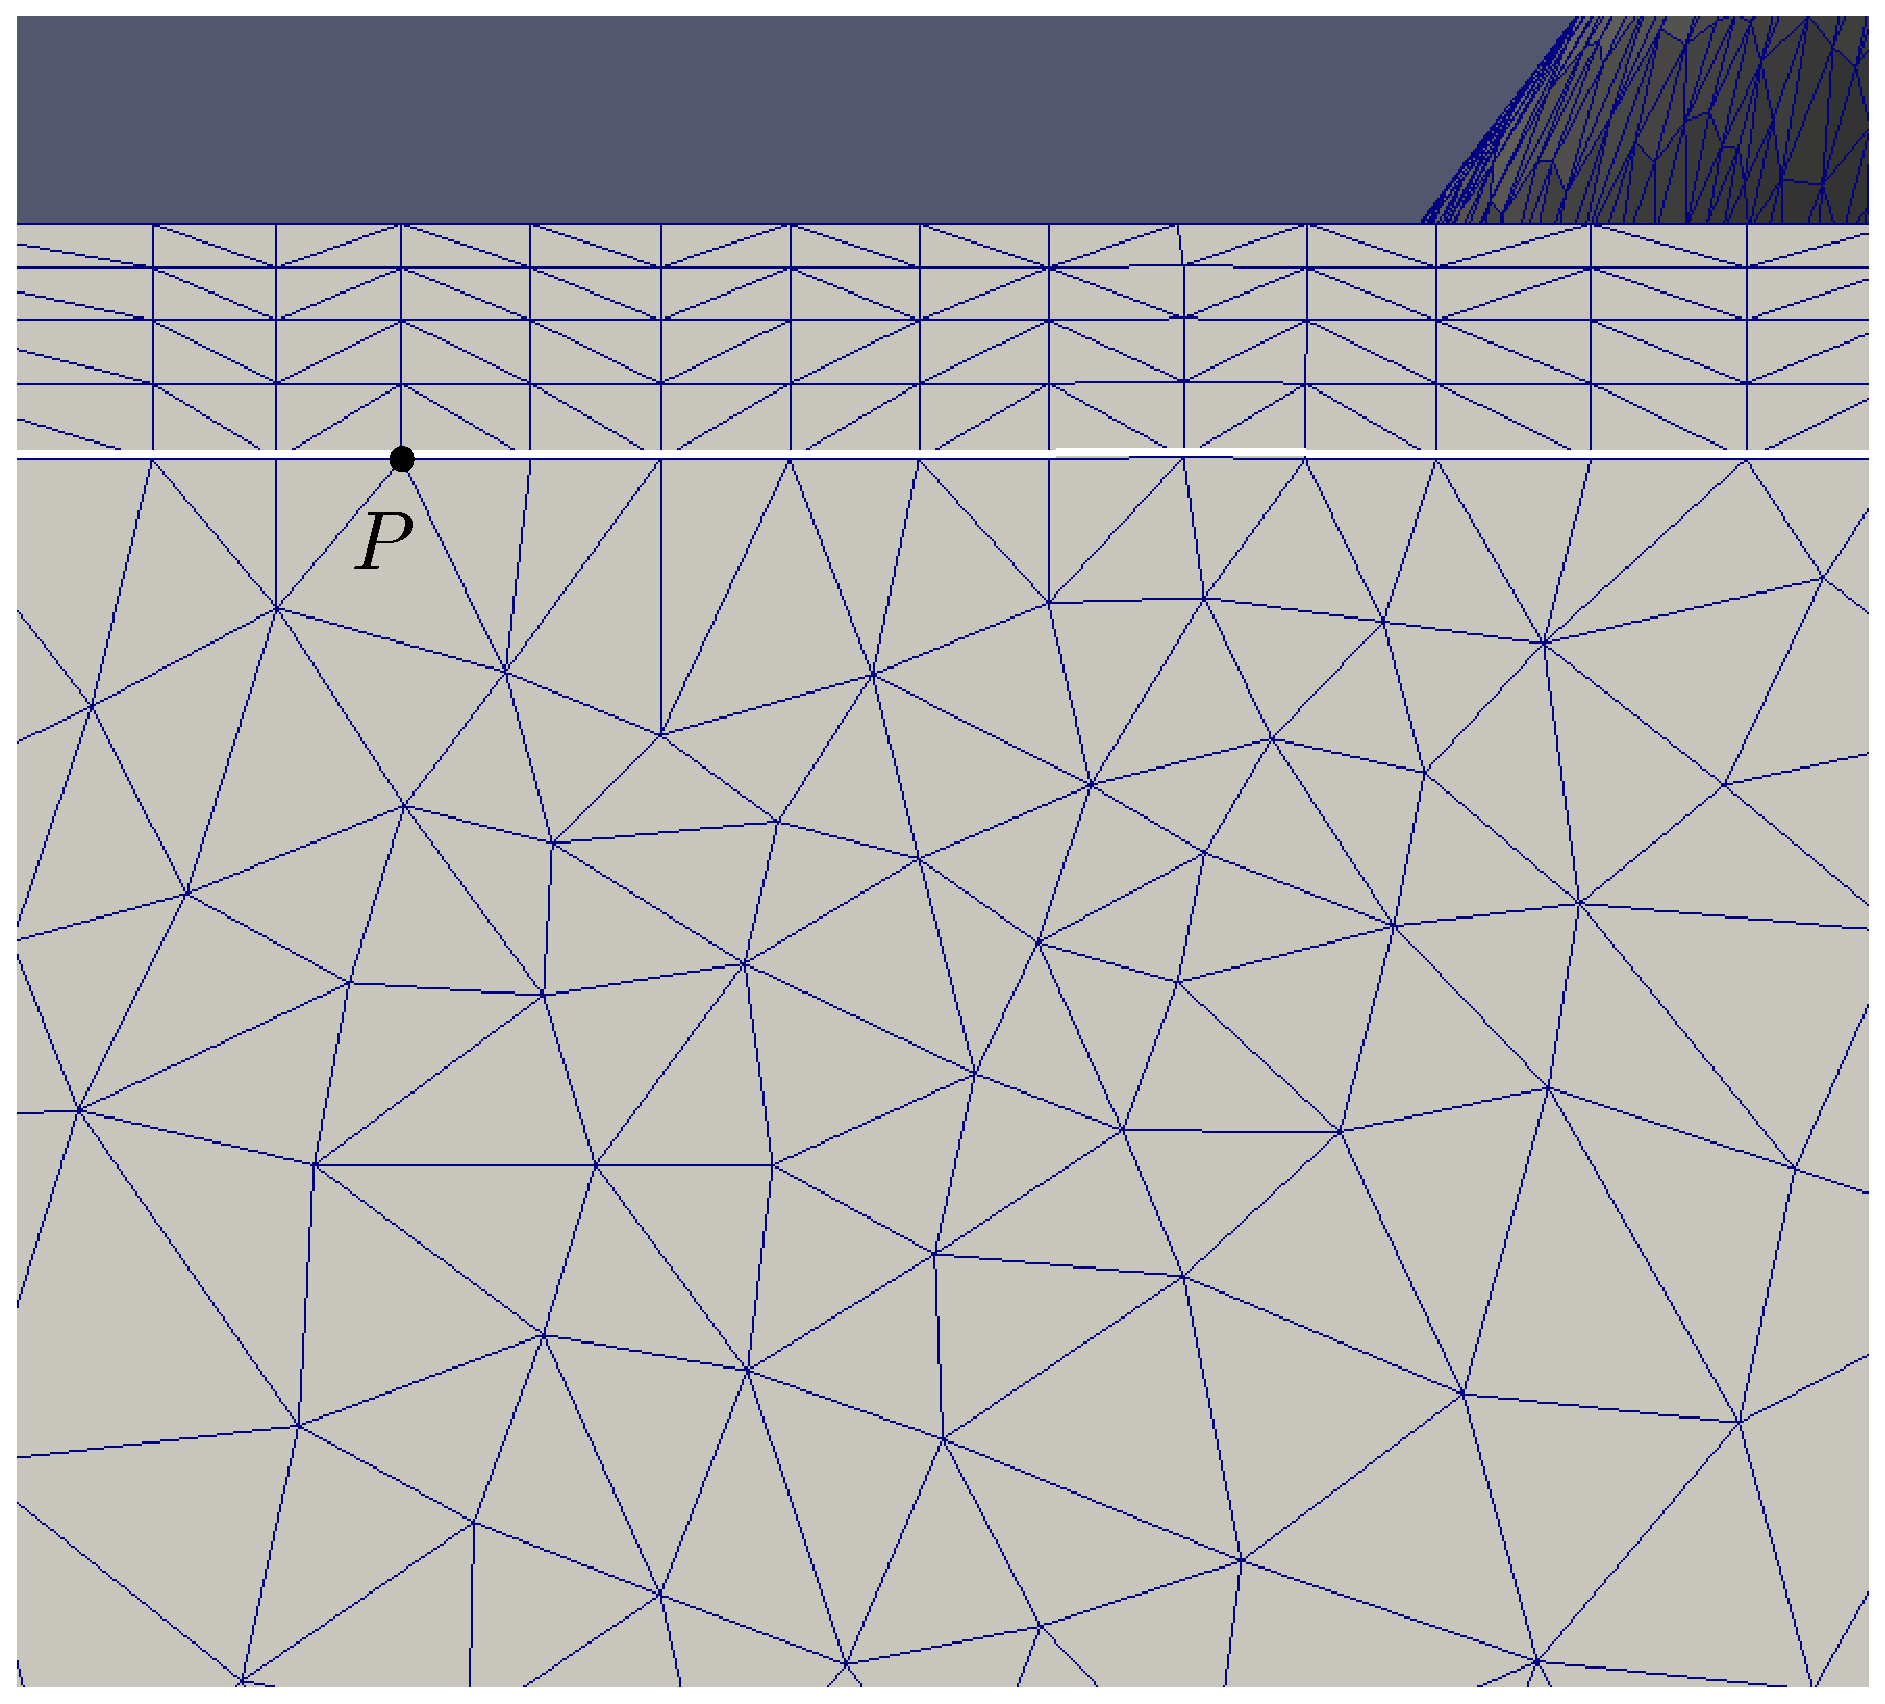
\includegraphics[width=.9\linewidth]{interior-vert-collapse/cc4.eps}
  \caption{}
  \label{cc4}
\end{subfigure}
\caption{Interior vertex decimation through edge collapse. The highlighted line shows the advancing front. In (a), vertex $P_2$ is about to encroach the front. Hence, the best vertex for collapse is chosen among its neighbours. The best vertex for edge collapse here is $P_1$. Hence, $P_2$ is collapsed on to $P_1$. The connectivity after the edge collapse is shown in (b) where vertex $P$ represents the collapsed vertex. Similarly, in (c), vertex $P_2$ is about to encroach the advancing front and is collapsed onto vertex $P_1$ which is on the advancing front itself. The new connectivity is shown in (d) where all the possibly encroaching vertices for the advancing layer are decimated.}
\label{interior-vert-collapse}
\end{figure}



\subsection{Front Collision and Redefinition}

Till now we have described how points advance in layers and how are the layers recovered after each advancing layer step. However, some points on the advancing layer might encroach another edge on the advancing front. In other words, a point in the advancing front might come too close to other points(or edges) on the front which might result in encroachment if we advance all the points in the current layer to the next one. To tackle this issue, we preemptively identify such points and redefine the front so as to avoid encroachments. The redefinition process results in termination of the marching process for some or all the points on the advancing front.

To achieve the goal of front redefinition, we first iterate through all the points in the front to identify the encroached points. These points are the ones whose distance from any edge in the front, except its adjacent edges, is less than $2.4$ times the extrusion length at that point. As our surface mesh is closed, we can utilize vertex connectivity to find out possible vertex-front edge encroachment. Hence, for a given point on the advancing front, only the edges on the front that share a triangle with that point are checked for encroachment. This saves a lot of computational cost while identifying encroached vertices. This is assuming that the input triangulation is fine enough to resolve the complex features of the geometry so that we don't have to iterate through all the edges to find whether a given point is encroached. 

After these encroached points and their corresponding encroached edges are identified, we reconnect the non-encroached points so as to form the new front. The encroached points are moved out of the advancing front and the front is hence redefined. An example of front redefinition can be seen in Figure \ref{front-redef}. Here, the red line denotes the old front. If two of the three corner points are marched on to the next layer, the mesh elements would overlap each other and the front would be invalidated. Hence, two of them are selected to be moved out of the front. The front is redefined to contain the adjacent edges of only the remaining vertices in the front. The green line shows the newly defined front which would be used for the generation of the next layer on the surface.

\begin{figure}[hbt!]
    \centering
    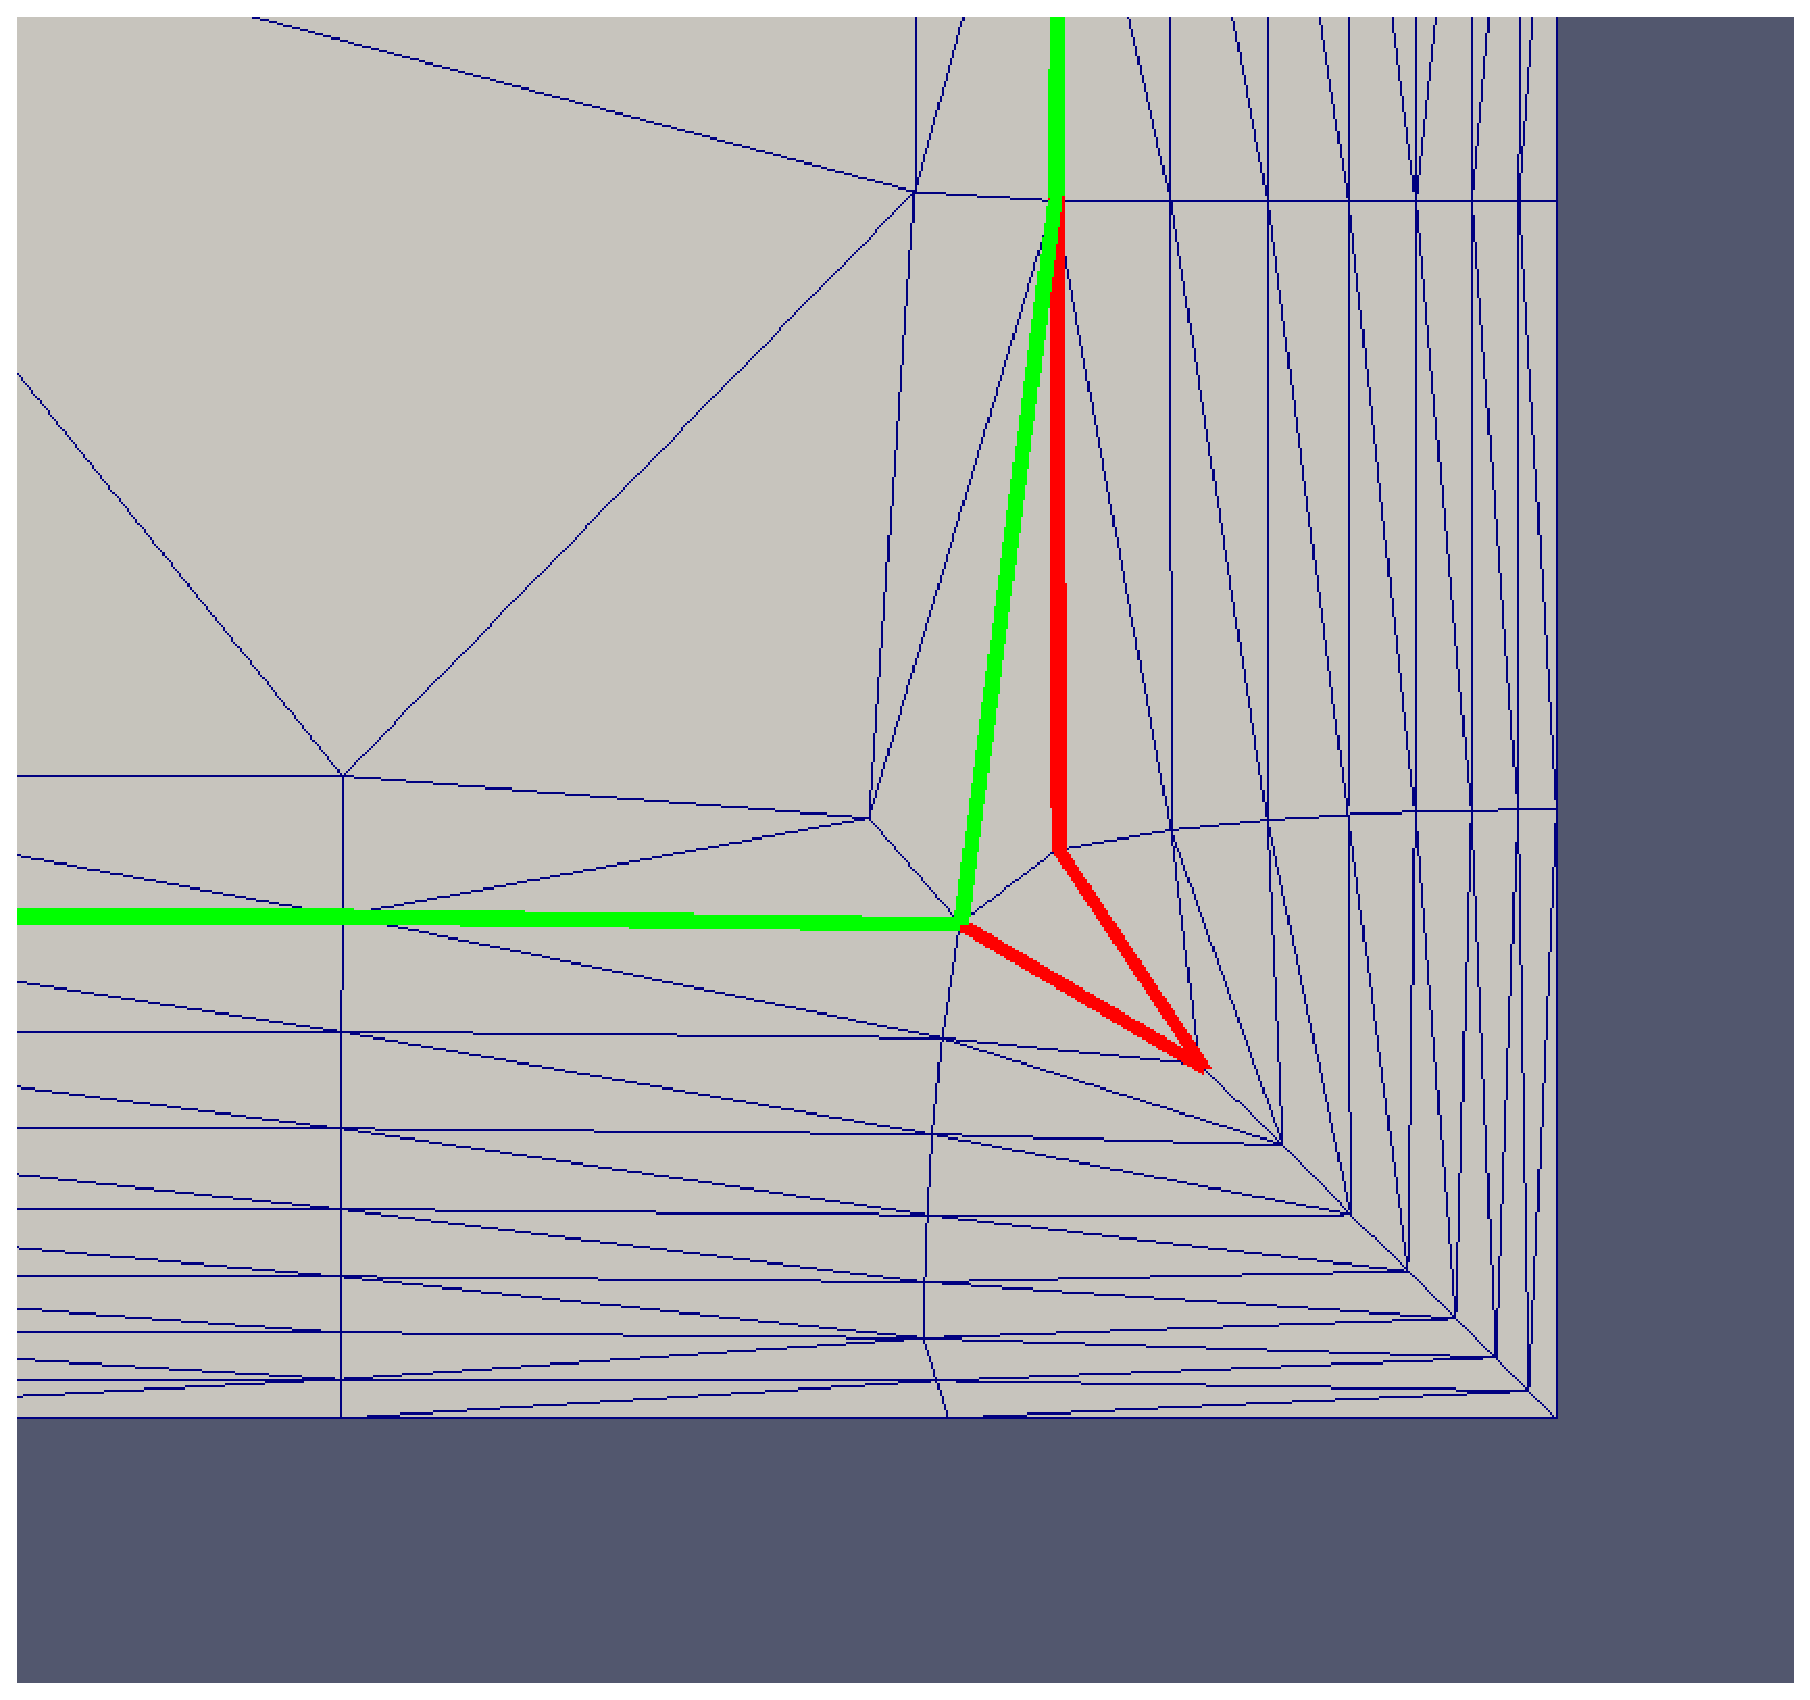
\includegraphics[width=.5\textwidth]{front-before-n-after-redefinition.eps}
    \caption{Zoomed in view of an advancing layer mesh. After advancing a few layers, the mesh reaches the front denoted by red line. If the mesh keeps advancing like this, the front would collapse on itself resulting in undefined behaviour. The front redefinition routine stops two points from marching further and redefines the front as shown in green. The next marched layer is also shown.}
    \label{front-redef}
\end{figure}

\subsection{Combining Triangular Elements to Quads}

Generating advancing layers over the surface proceeds by inserting points in the initial triangulation. After generating a layer of the mesh, we can combine the triangular cells into quadrilateral cells by removing the edges from the mesh. Edges are removed from the finished layers so as to generate superior quality quadrilateral cells. As the layers advance from the boundary towards the tangential direction onto the surface, the quadrilateral elements generated retain the boundary topology several layers into the interior of the surface. The quality of a quadrilateral element is calculated as the inverse of the maximum deviation of its interior angle from 90 degrees. This criterion is selected so as to prefer rectangular elements and retain the boundary representation on the surface mesh. Multiple iterations of this subroutine is run for the same layer during mesh generation to ensure as few triangular elements are generated per layer as possible.

%TODO: add a figure demonstrating the combine tri to quad subroutine

\subsection{Smoothing}

Applying a smoothing methodology to a boundary layer mesh is non-trivial. On the one hand, smoothing improves the mesh element quality, while on the other hand it can diffuse the boundary topology in the advancing layers of the mesh. Hence, a simple Laplacian smoothing will not serve the purpose. Optimization based approaches could be employed to smooth the mesh by moving the mesh nodes so as to maximize a quality metric\cite{canann1998approach}. However, even in such approaches, the boundary layers of the mesh are kept fixed and the isotropic regions of the mesh are smoothed. Additionally, this approach is quite computationally intensive. The smoothing methodology that we use for the advancing layer mesh is physically-based smoothing. The mesh nodes exert forces on each other and hence, each mesh node is moved so as to balance out all the forces. This procedure of smoothing is also called as spring based smoothing as the edges of the mesh act as springs which pull or push the mesh nodes away or towards each other.

Several spring forces are applied to a given mesh node in the smoothing procedure. Each spring constant is denoted by $k_{spring}$. The forces are -

\begin{itemize}
\item \textbf{Parent force} - force which keeps the distance of the vertex to its parent (from which it was extruded) closer to the initial extrusion length($l_{ideal}$) between the two.
\begin{equation}
f_{parent} = k_{extrusion} * \frac{l_{real} - l_{ideal}}{l_{real} + l_{ideal}} * (parentLocation - vertLocation)
\end{equation}
\item \textbf{Kid force} - similar to the parent force, this one keeps the distance between the node and its kid closer to the initial extrusion length.
\begin{equation}
f_{kid} = k_{extrusion} * \frac{l_{real} - l_{ideal}}{l_{real} + l_{ideal}} * (kidLocation - vertLocation)
\end{equation}
\item \textbf{Neighbour force} - force to maintain uniform spacing of mesh nodes for each layer.
\begin{equation}
f_{neighbour} = k_{neighbour} * \frac{(vertLocation - leftVertLocation) + (vertLocation - rightVertLocation)}{ 2.0};
\end{equation}
\item \textbf{Original location} - a force is added to restrict the movement of the vertex from the location at which it was placed in the mesh before smoothing. This term also ensures that the deviation of the mesh nodes from the initial surface representation is as little as possible.
\begin{equation}
f_{original} = k_{original} * (origialLocation - currentLocation)
\end{equation}
\begin{equation}
\end{equation}
\end{itemize}

These forces are summed up to give the mesh node a resultant force and the node is moved according to the total force. Several iterations (around 5-10) of smoothing are done per layer as the mesh advances towards surface interior. A limit is set to the vertex movement per smoothing iteration. The distance a vertex moves per iteration of the smoothing algorithm is kept at $5\%$ of the extrusion length at that vertex. This helps in limiting the movement of the vertex when the initial boundary discretization is too coarse.

\begin{figure}
\centering
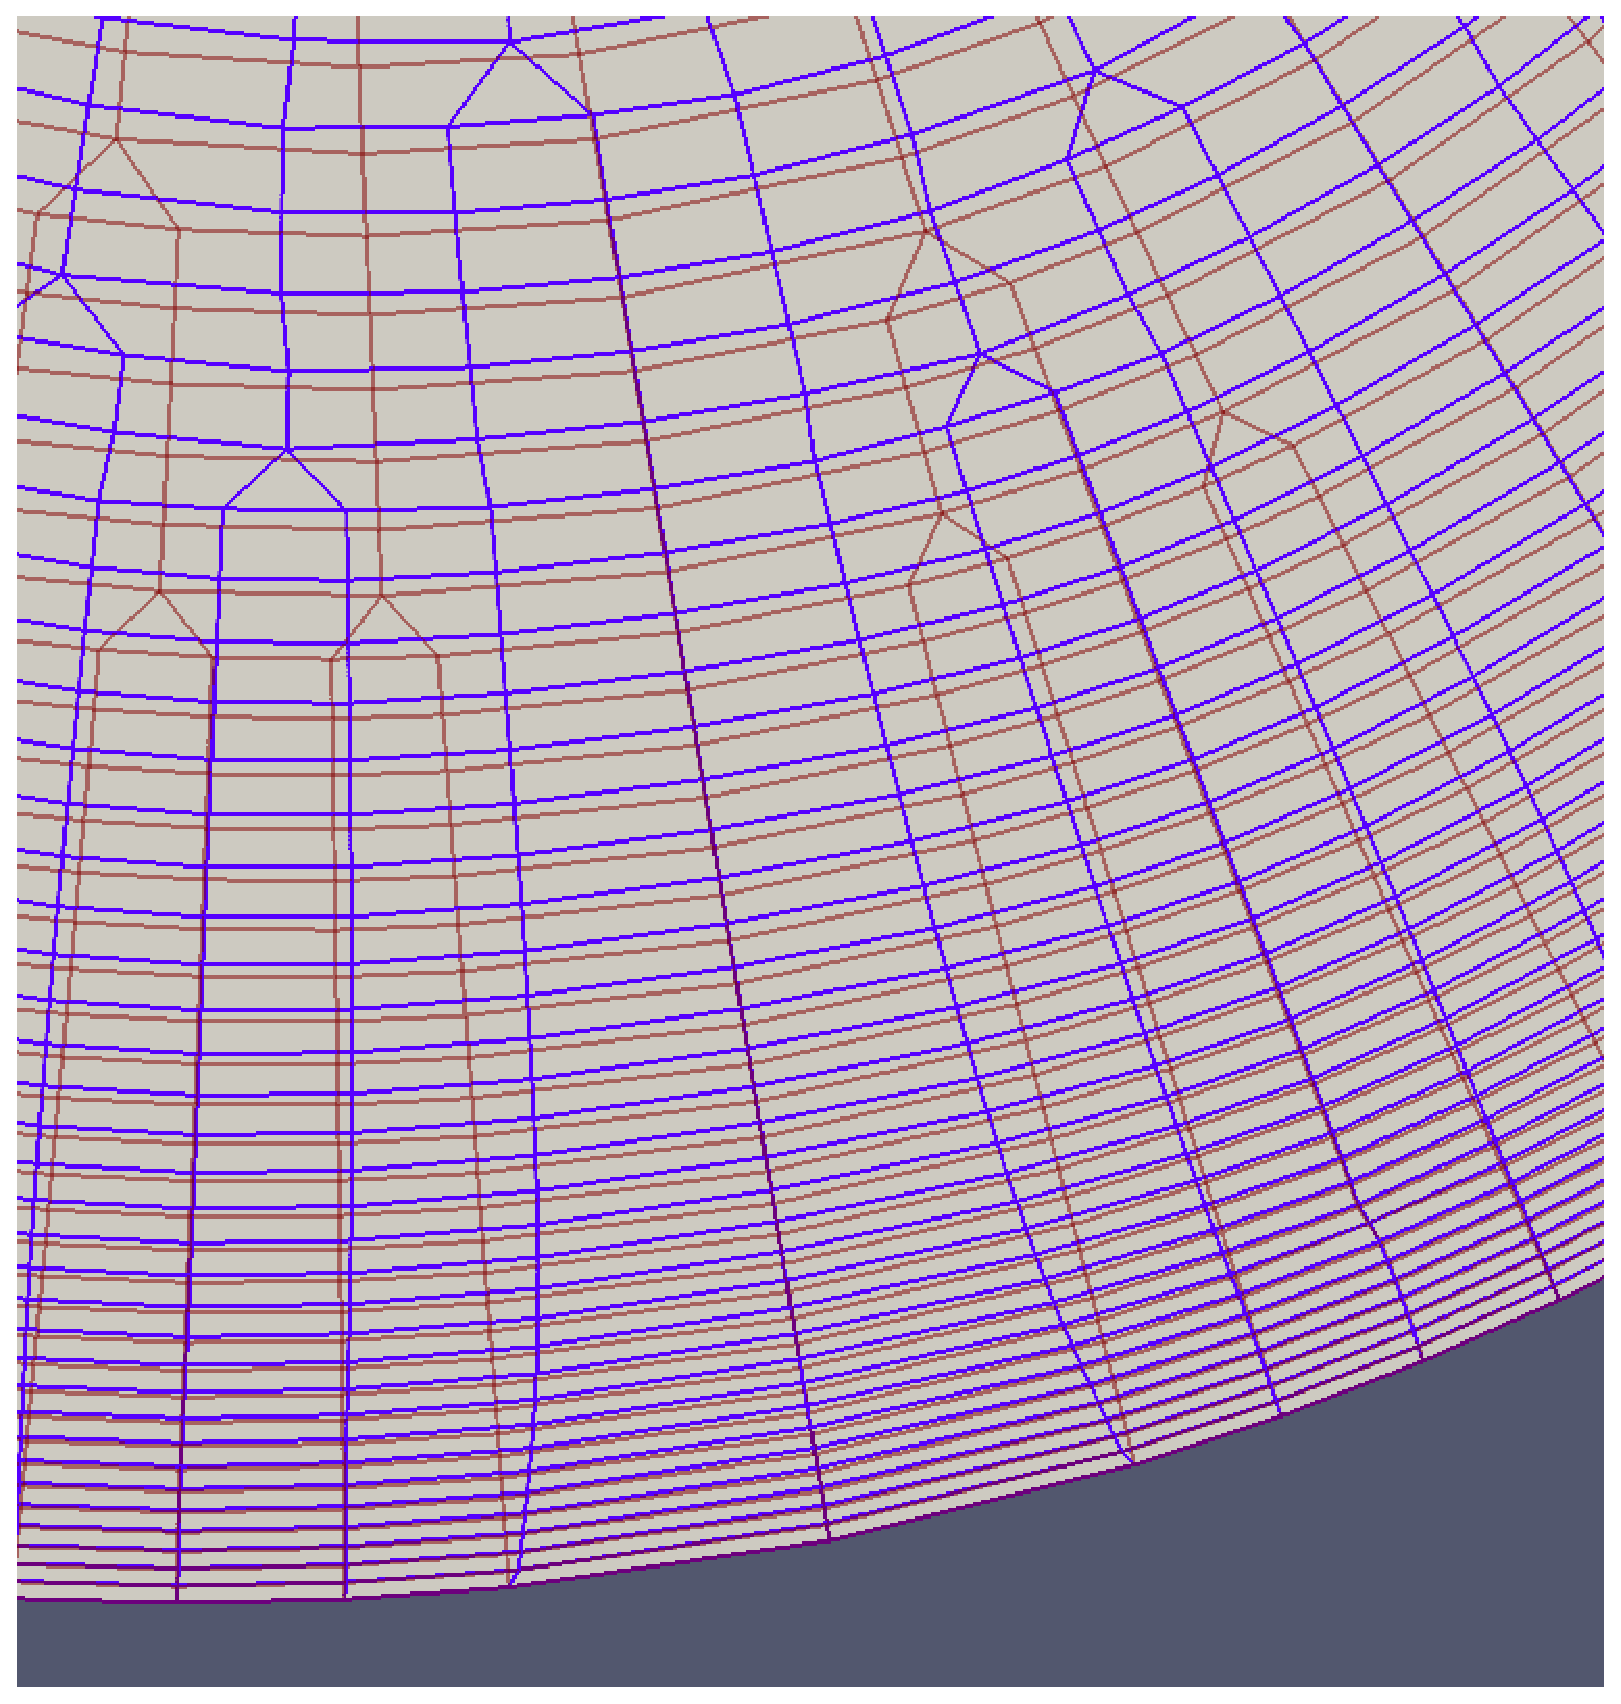
\includegraphics[scale=0.3]{smoothing/smoothing-comparison-cylinder-cap.eps}
\caption{Zoomed in view of smoothing applied to an advancing layer surface mesh. Dark blue lines represent smooth mesh and flat red lines represent the mesh without smoothing. We can see that the smoothed version of the mesh helps to attain uniform aspect ratio at each layer.}
\label{fig-smoothing-cylinder}
\end{figure}
%TODO: Mesh smoothing add a figure

\section{Overall Mesh Generation Algorithm}

In the previous section, we have detailed the steps in the advancing layer mesh generation routine. Here, we summarize the algorithm in the form of a pseudo code in Algorithm \ref{algo}.

\begin{algorithm}[hbt!]
\caption{Overall Mesh Generation algorithm}\label{alg:euclid}
\begin{algorithmic}[1]
\Procedure{SurfMesh::CreateMesh}{triangulation $T,$ extrusion length, growth ratio}
\State Create surface geometry $S \gets T$
\State Initialize Advancing Layer $F$ from Surface Boundary
\While{ $F\neq\emptyset$}\Comment{Advance until Front $F$ isn't empty}
\State \textsc{AdvanceLayer($F$)}
\State Validate the new Layer
\EndWhile \label{advancing-layer-routine}
\State Export \textsc{SurfMesh}
\EndProcedure
\Procedure{SurfMesh::AdvanceLayer}{$F$}
\State Delete Encroaching Interior Vertices
\State Redefine front $F$ Until No Vertex Encroachment
\State Extrude All Points of $F$ and Insert Into Mesh
\State Recover front $F'$ \Comment{Through forced edge creation between kid vertices}
\State Improve Mesh Quality by Edge Swapping \Comment{In the immediate interior of mesh}
\State Collapse Short Edges in the Front
\State Update Extrusion Length for vertices
\EndProcedure
\end{algorithmic}
\label{algo}
\end{algorithm}

\section{Assumptions}

We make a few assumptions on the input triangulation for our mesh generation algorithm to successfully create a valid mesh. The first one is that the triangulation of the surface is fine enough to resolve the geometric complexities in the object. If the input triangulation is too coarse, the encroaching interior vertex deletion subroutine will create mesh elements that deviate significantly from the surface or even fail. Hence, for highly curved regions of the surface, the input triangulation should be within 30 degrees deviation of the surface. However, this issue can be tackled by refining the triangulation using any isotropic refinement algorithm as long as it retains the features of the input object. Coarse triangulations are acceptable for objects without any geometric complexities.

Another assumption we have made for the input triangulation is that it would have well defined boundaries where the advancing layers can march out from. For future, we intend to incorporate a subroutine that identifies these boundaries even on objects which don't have well defined features, for eg. leading edge of an airfoil. Accepting boundary elements as a user input is also an option for such objects.

\section{Examples}

We use the surface mesh generation algorithm described here to mesh some geometries. We illustrate how the advancing layer algorithm works by creating several advancing fronts from the boundary of input triangulation. Figure \ref{cyl-coarse} shows a cylindrical object with a coarse boundary and surface discretization. The object contains three sub-surfaces. These include the planar end caps of the cylinder and the curved cylindrical surface. The three sub-surfaces of the input triangulation are segmented and meshed  independently using the advancing front surface generation routine. Resultant mesh is shown in Figure \ref{cyl-coarse-mesh}. It can be seen that the boundary curves, that is the circular bounding curve of the sub-surfaces is preserved very well for several layers in the surface interior. Hence, the advancing layer surface mesh generation algorithm helps to preserve the boundary curve even for coarse initial surface discretization. Figure \ref{cyl-coarse-cap} and \ref{cyl-coarse-cap-mesh} show the initial triangulation and the final mesh for the end cap of the cylinder. 

Another example is shown in Figure \ref{cylinder-fine}. Here, the same cylindrical geometry is taken as the input but with a finer boundary and surface discretization as shown in Figure \ref{cyl-fine}. The surface mesh generated for this geometry is shown in Figure \ref{cyl-fine-mesh}. Here again, the advancing layers grow anisotropically from the boundary into the interior of the mesh and generate 16 layers on all the three sub-surfaces. The parameters used for both the meshes described for the cylindrical geometry are shown in Table \ref{cyl-table}. The value of aspect ratio at the surface boundary is set to $\approx 5-6$ to generate the anisotropic meshes. This value can be modified by changing the initial extrusion length and the growth ratio, which are the inputs to the algorithm. The number of layers generated on all three segmented surfaces of the coarse cylindrical geometry are 9 and for the fine cylindrical geometry are 16.

We demonstrate two more examples of advancing layer surface mesh generation. The first one is shown in Figure \ref{joint-surf5}. Here, one of the sub-surfaces of the geometry shown previously in Figure \ref{surf-segment} is meshed using the advancing layer surface mesh generation routine. The resultant mesh is shown in Figure \ref{surf5-joint-view2} and \ref{surf5-joint-view4}. The sub-surface boundary is highlighted in the figure. We can see that the regions close to surface boundaries have the required stretched elements having high aspect ratio. The aspect ratio for this mesh at the boundary varies with the boundary vertices but is set to be approximately 4-8. This gives us directional anisotropy as we move to surface interior from the boundaries of the mesh. Another example is shown in Figure \ref{twist}. Here, a twisted object with a coarse initial triangulation is input to the surface mesh generator. The object is segmented into three sub-surfaces which are meshed independently. We advance seven layers from the sub-surface boundaries to get a mesh which can be seen in Figure \ref{twist2}. A close up view on the mesh elements is shown in Figure \ref{twist4}. Here, the aspect ratio of the elements next to sub-surface boundaries is set to be approximately 12-20. These examples demonstrate the capability of the surface mesh generator to successfully advance multiple layers of anisotropic elements on a surface while preserving the boundary features.

\begin{figure}[hbt!]
\centering
\begin{subfigure}{.5\textwidth}
  \centering
  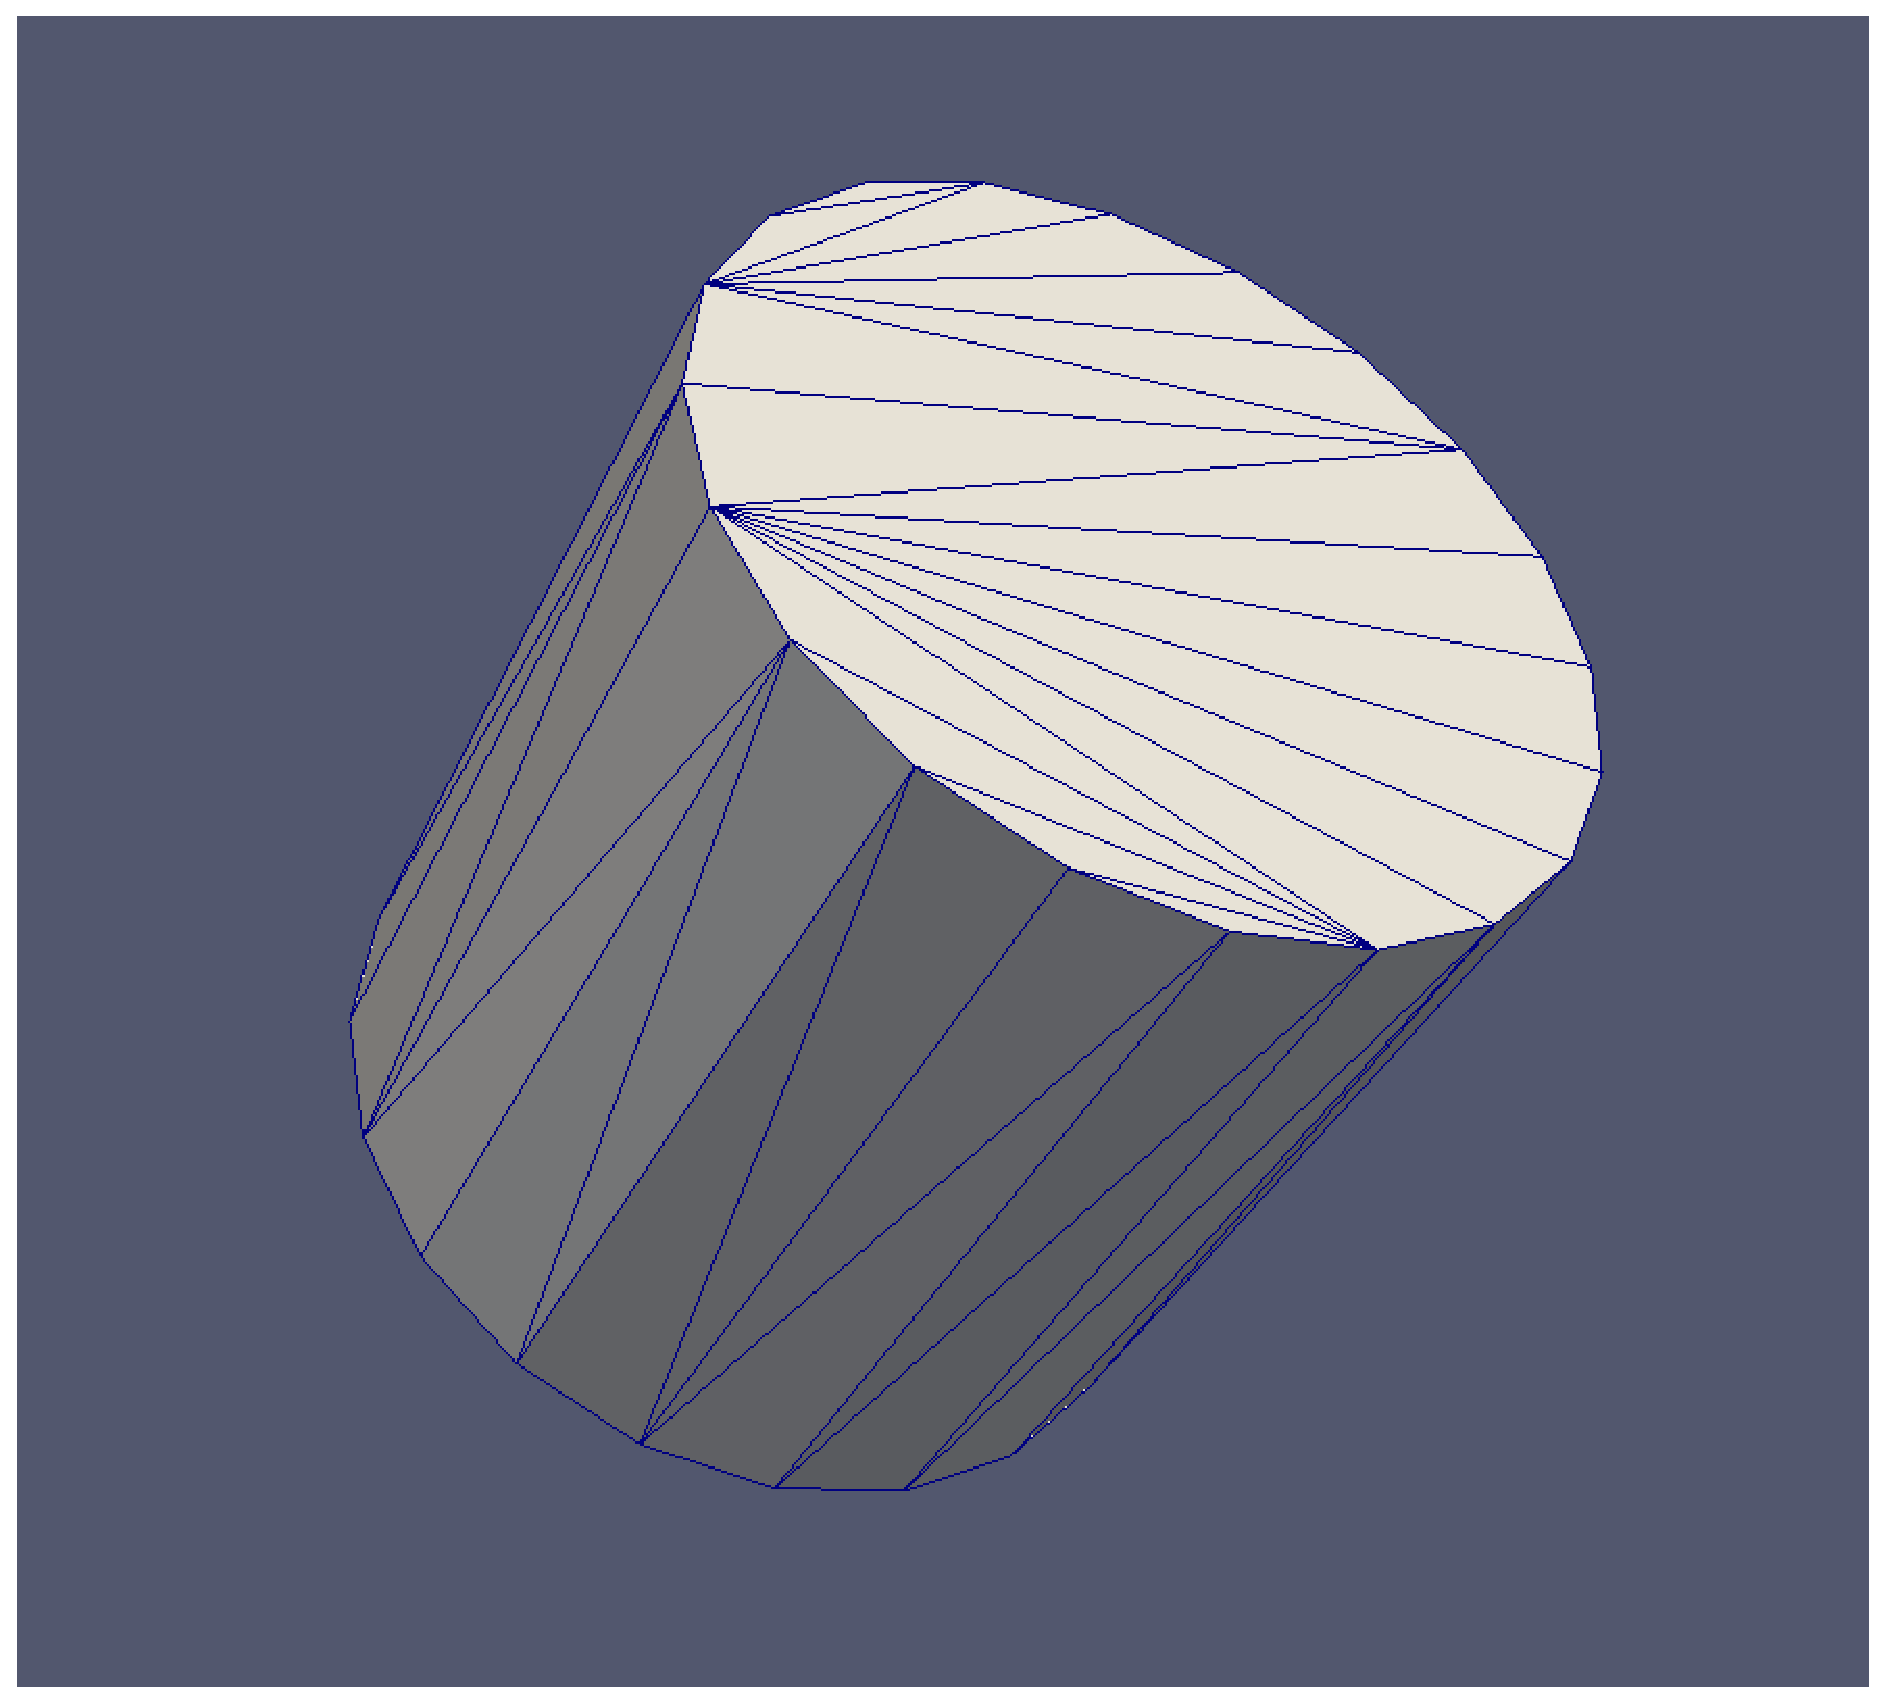
\includegraphics[width=.9\linewidth]{cylinder/coarse/cyl-coarse.eps}
  \caption{}
  \label{cyl-coarse}
\end{subfigure}%
\begin{subfigure}{.5\textwidth}
  \centering
  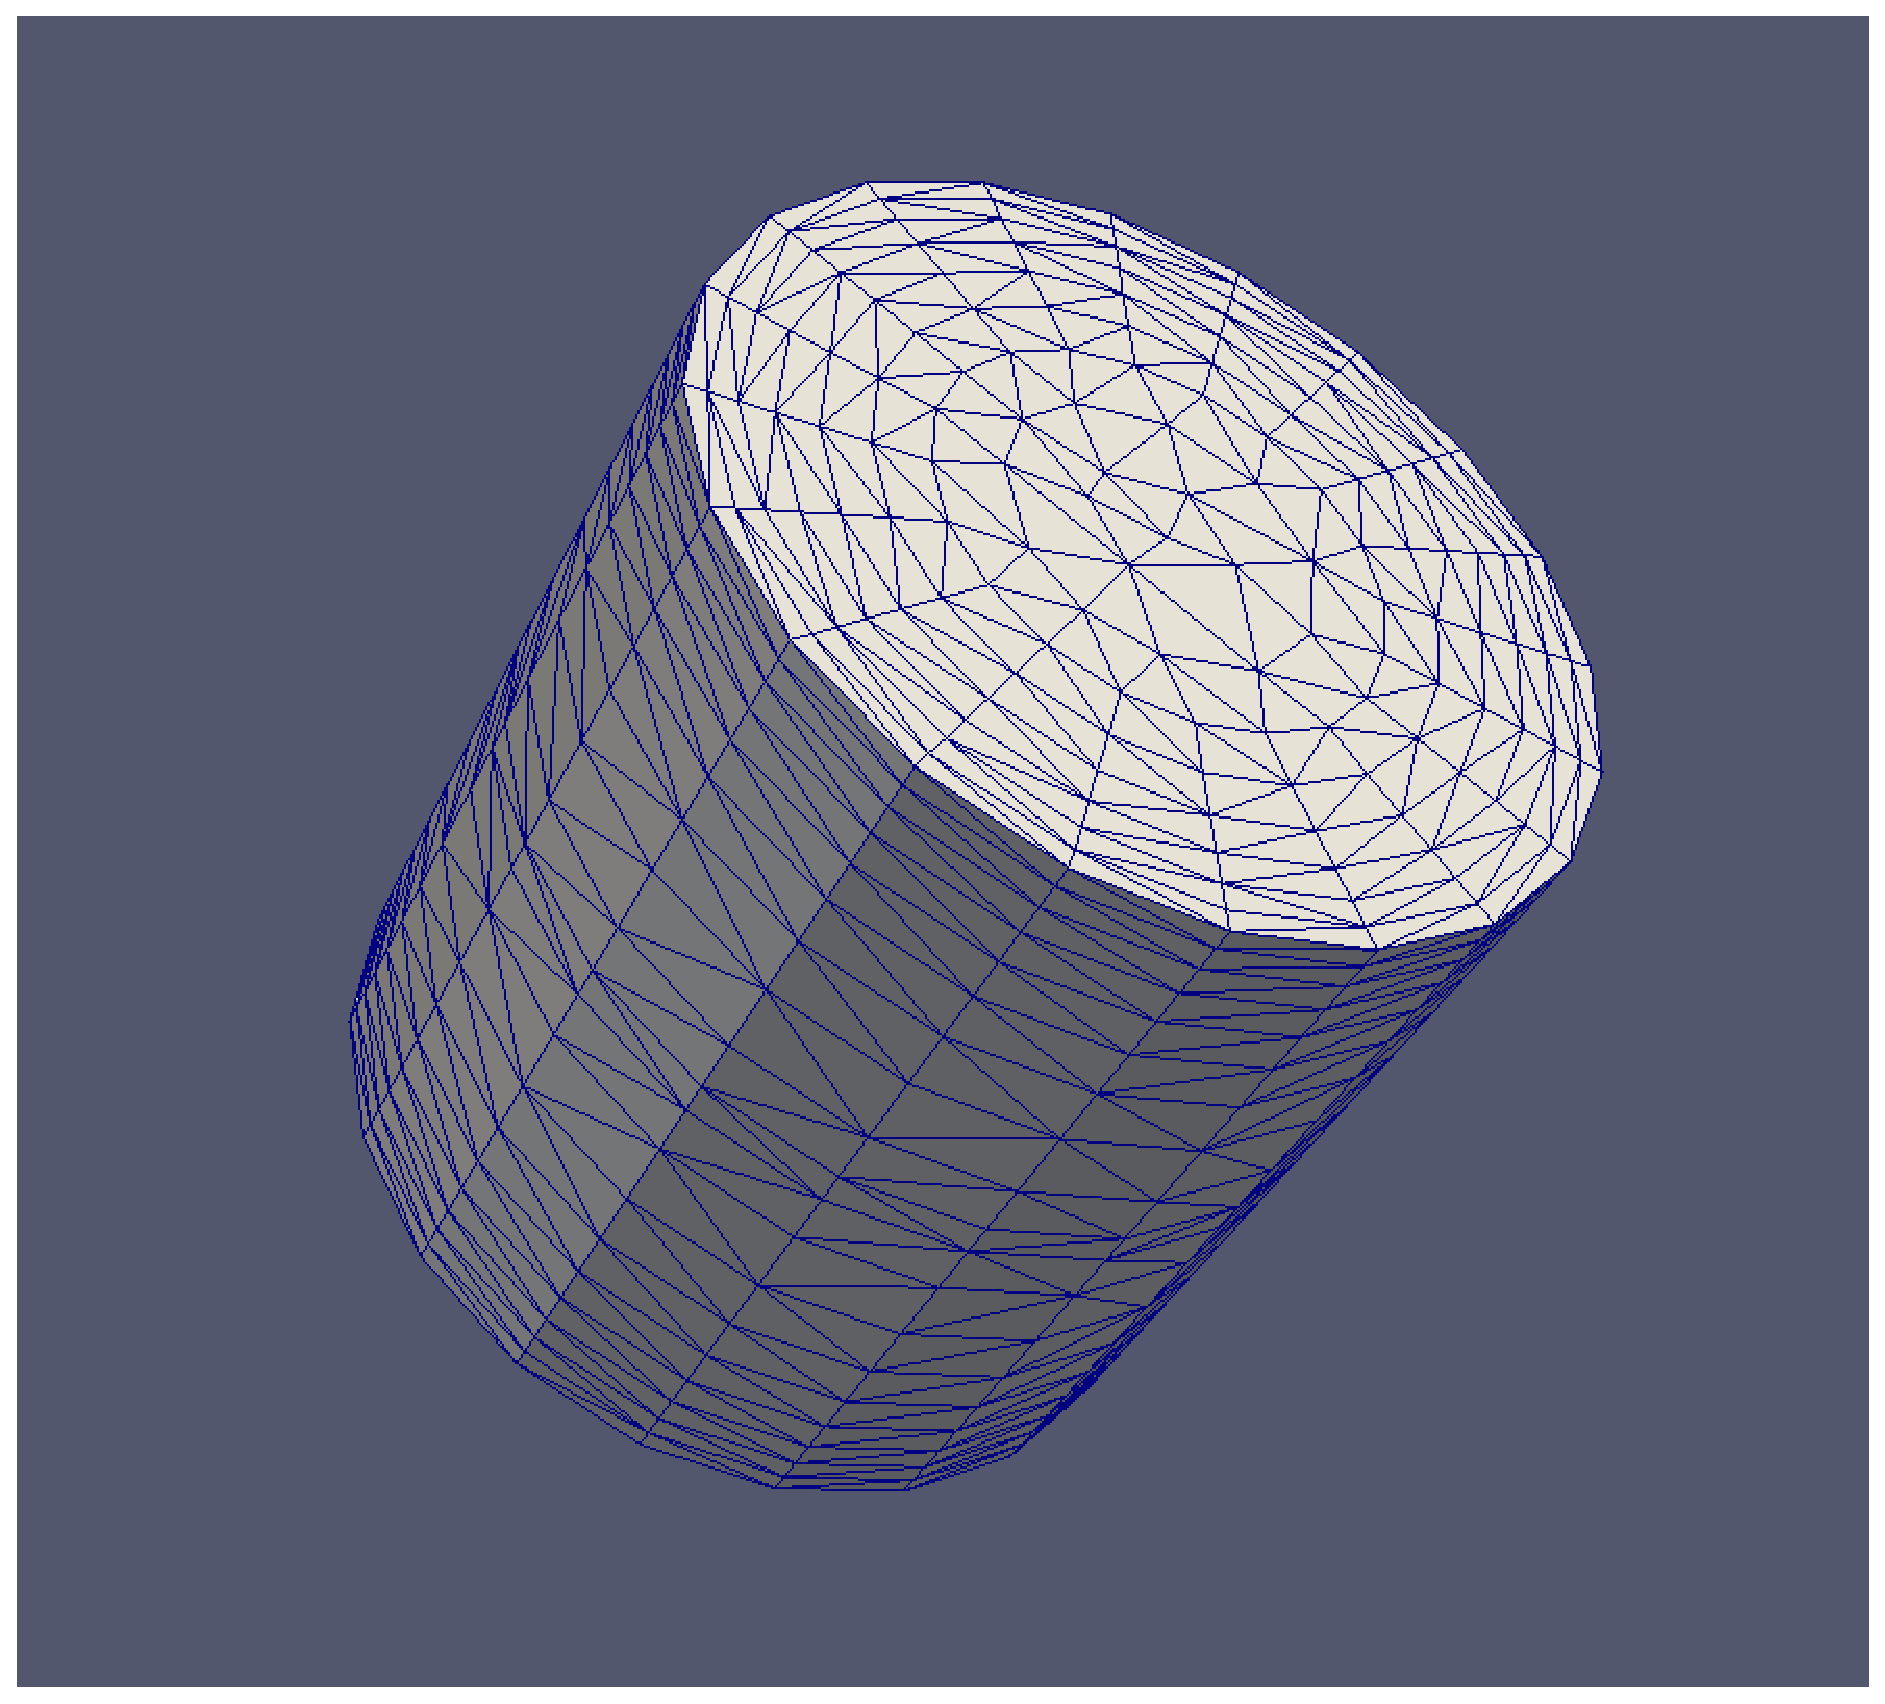
\includegraphics[width=.9\linewidth]{cylinder/coarse/cyl-coarse-mesh.eps}
  \caption{}
  \label{cyl-coarse-mesh}
\end{subfigure}
\begin{subfigure}{.5\textwidth}
  \centering
  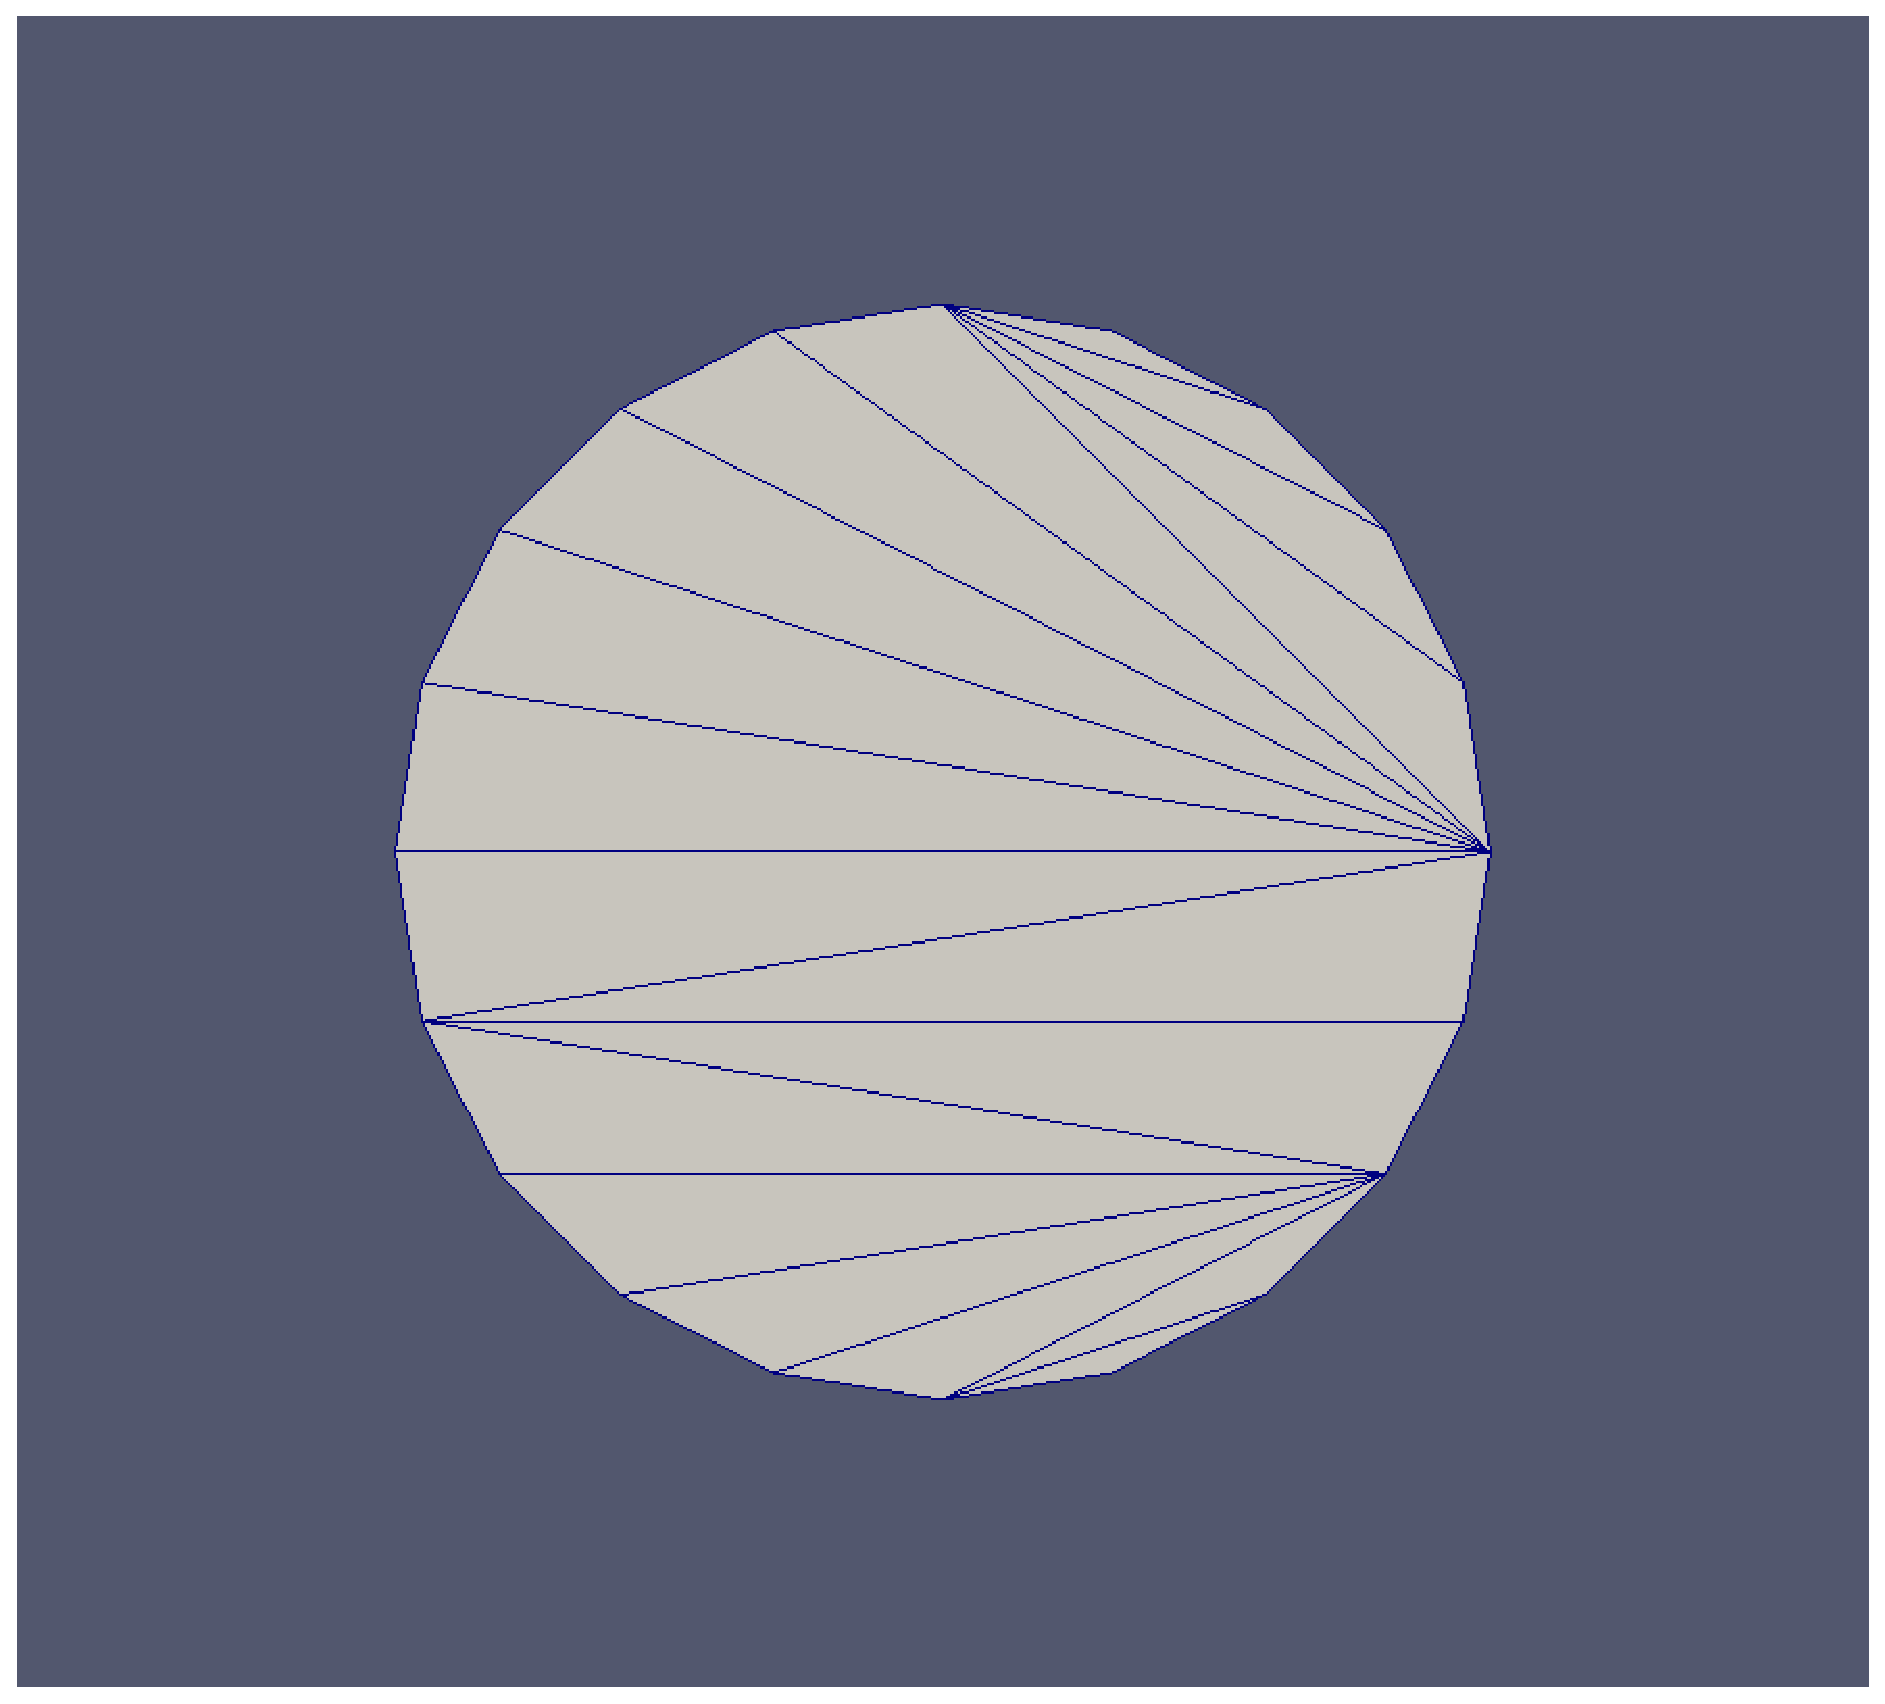
\includegraphics[width=.9\linewidth]{cylinder/coarse/cyl-coarse-cap.eps}
  \caption{}
  \label{cyl-coarse-cap}
\end{subfigure}%
\begin{subfigure}{.5\textwidth}
  \centering
  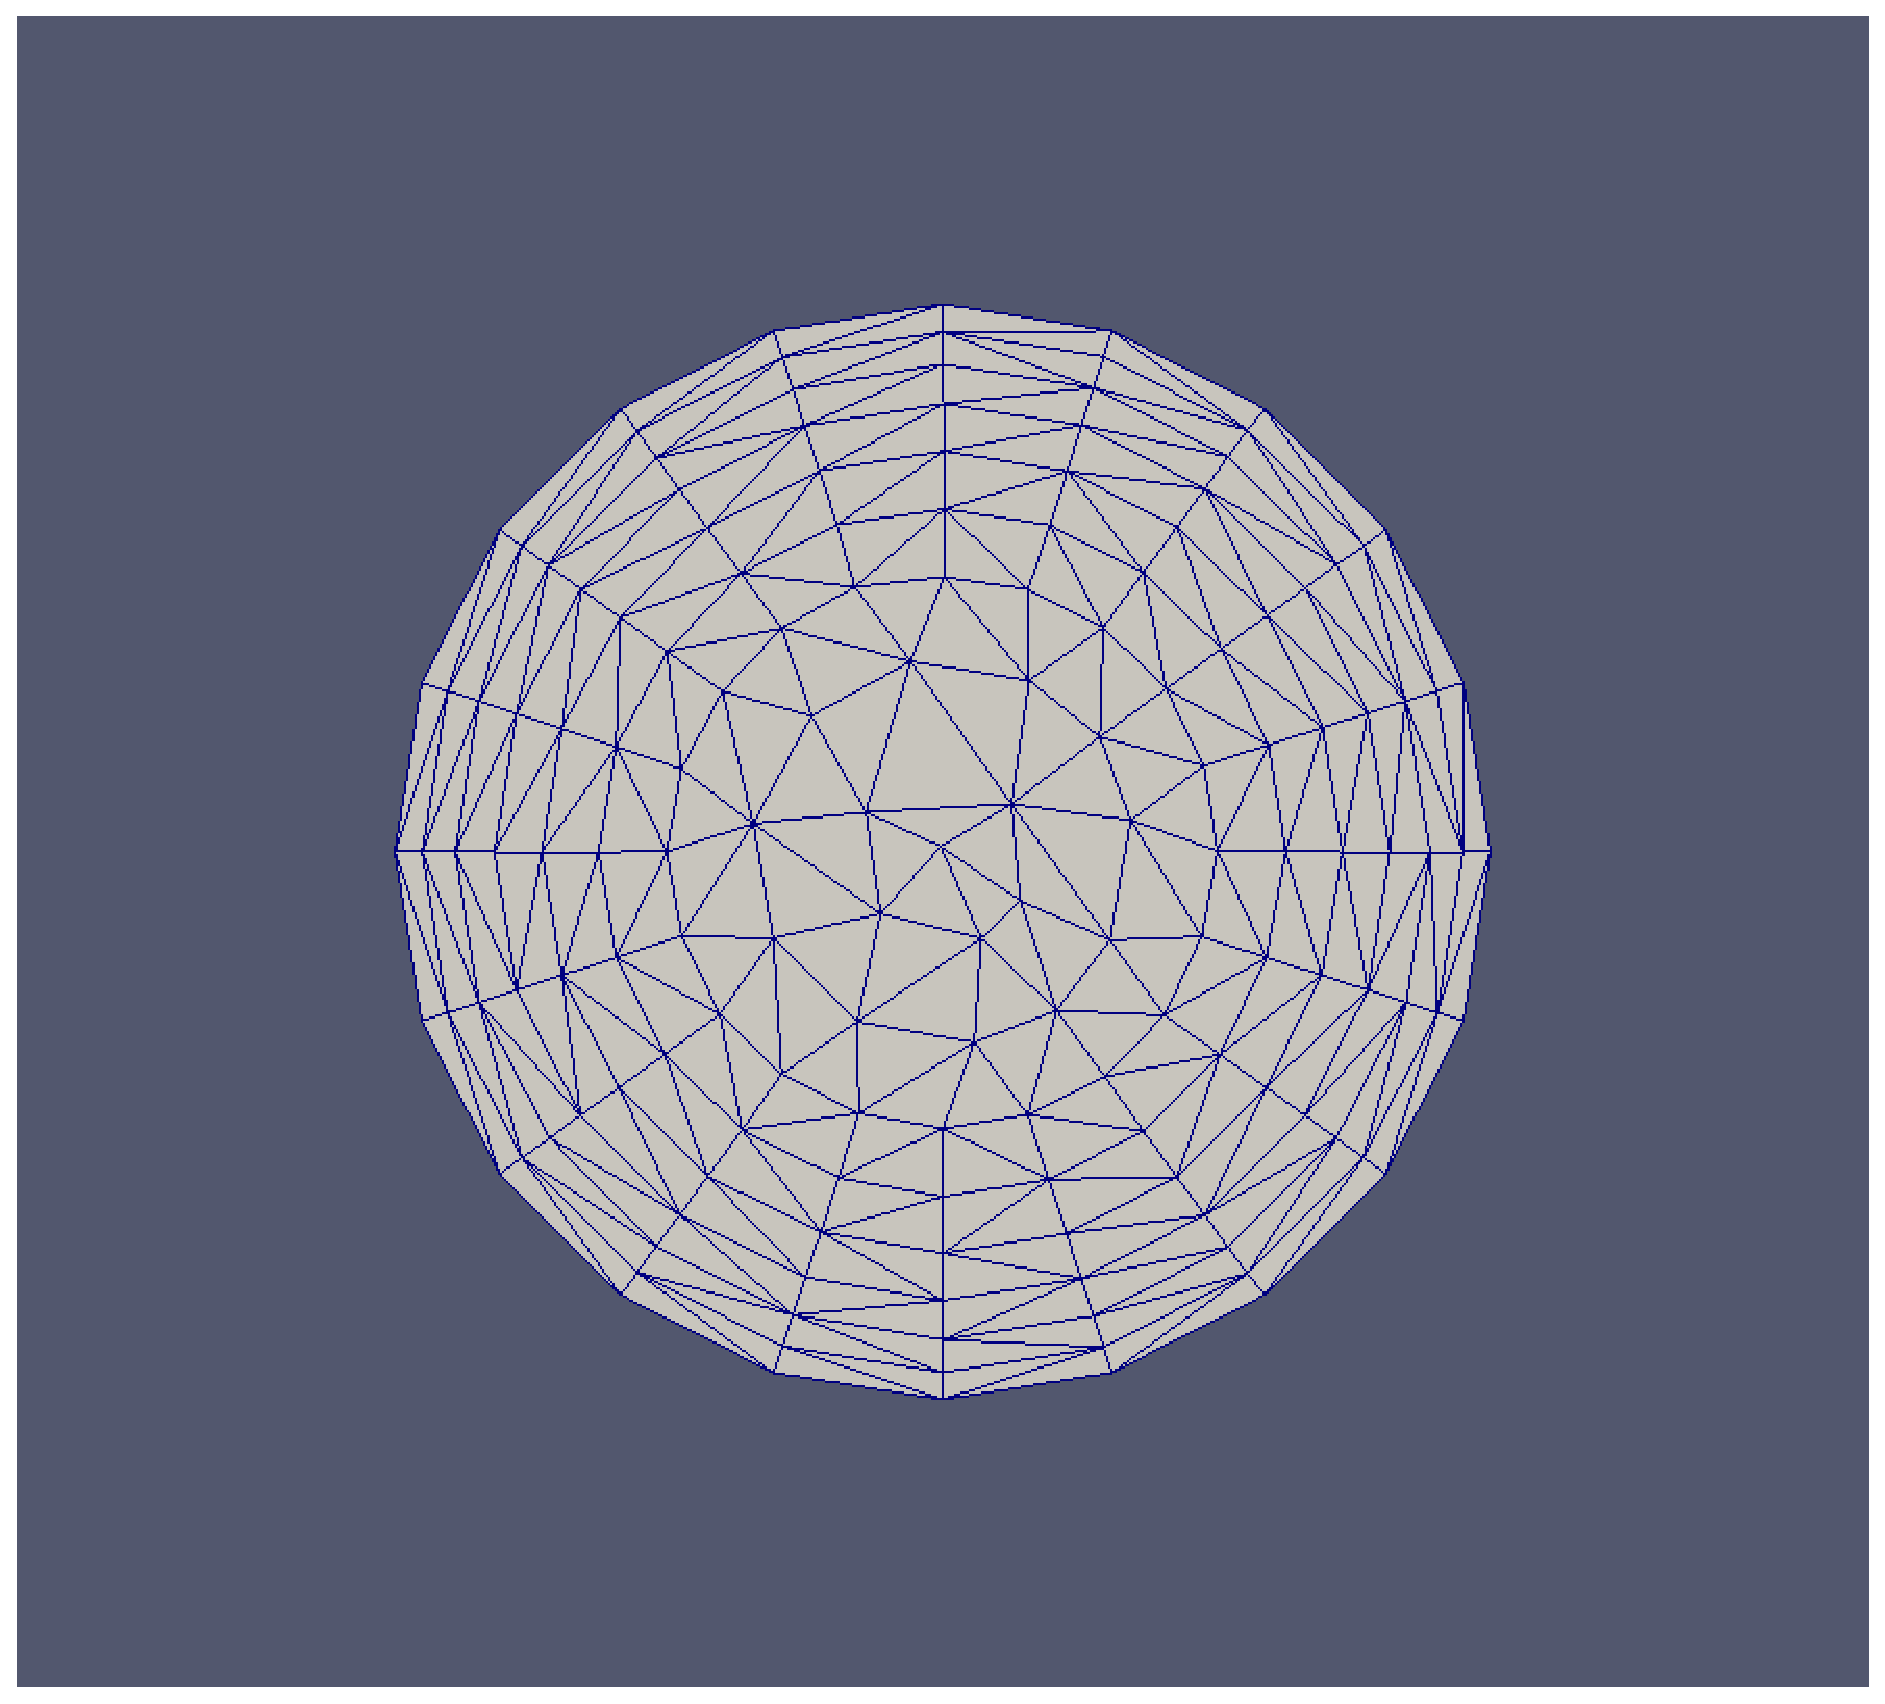
\includegraphics[width=.9\linewidth]{cylinder/coarse/cylinder-coarse-cap-mesh.eps}
  \caption{}
  \label{cyl-coarse-cap-mesh}
\end{subfigure}
\caption{Advancing layer mesh for a cylindrical object. (a) and (c) show the isometric view and the end cap of the initial surface discretization of the object. (b) and (d) show the surface mesh produced by the advancing layer routine.}
\label{cylinder}
\end{figure}


\begin{figure}[hbt!]
\centering
\begin{subfigure}{.5\textwidth}
  \centering
  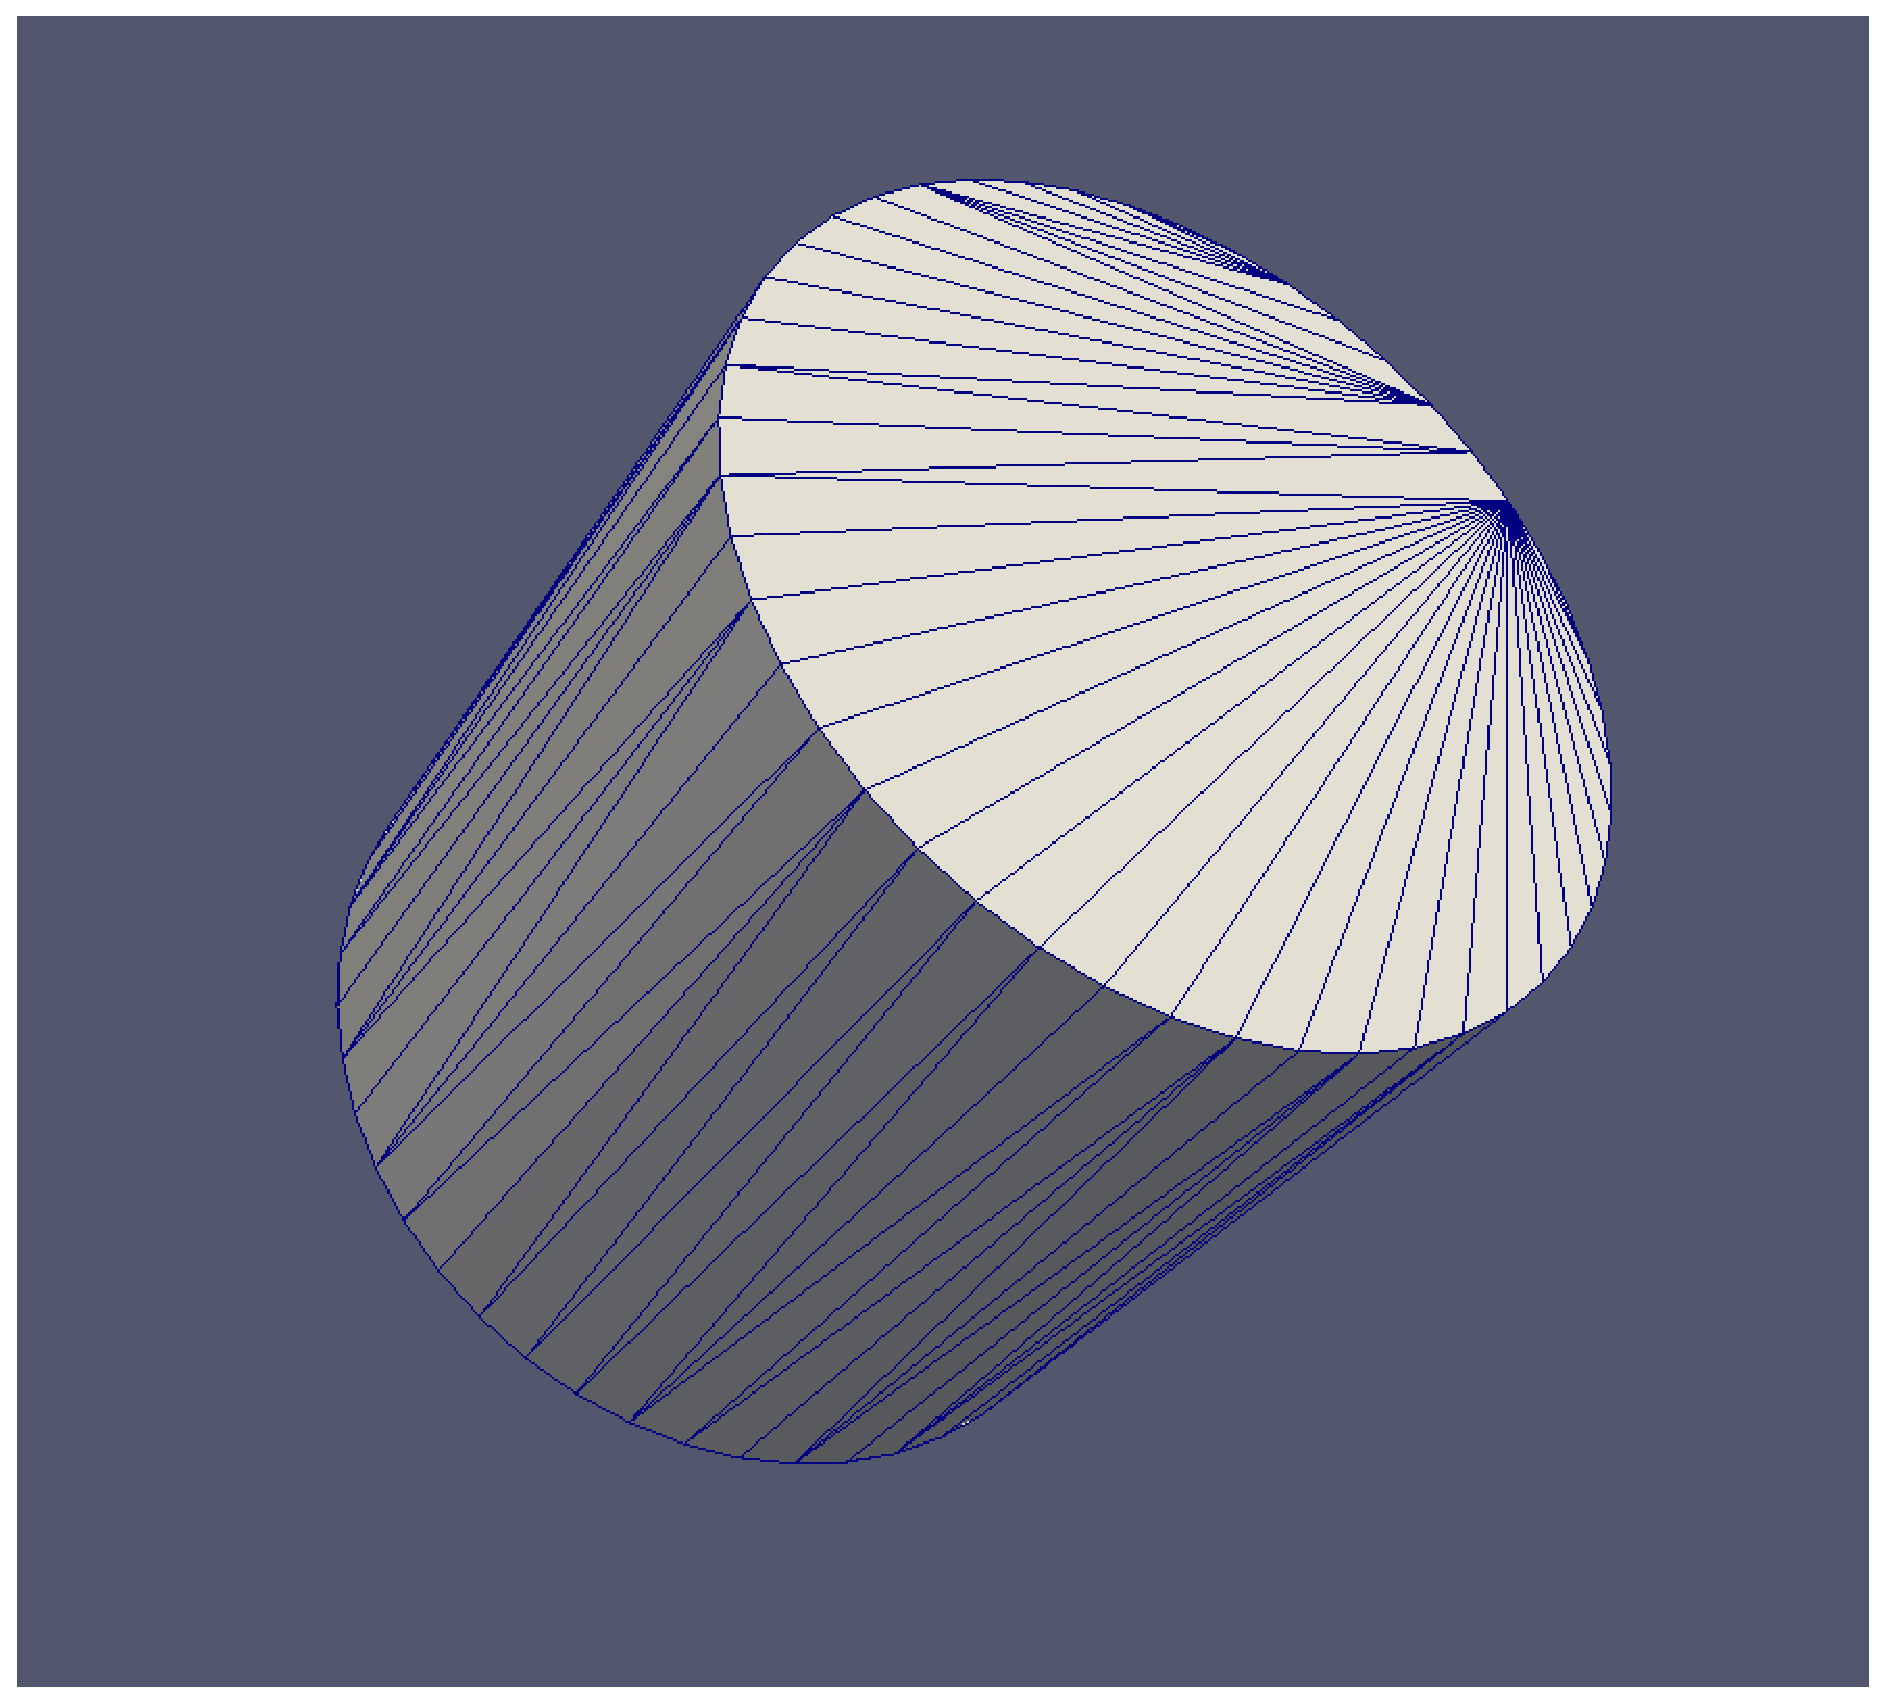
\includegraphics[width=.9\linewidth]{cylinder/fine/cyl-fine.eps}
  \caption{}
  \label{cyl-fine}
\end{subfigure}%
\begin{subfigure}{.5\textwidth}
  \centering
  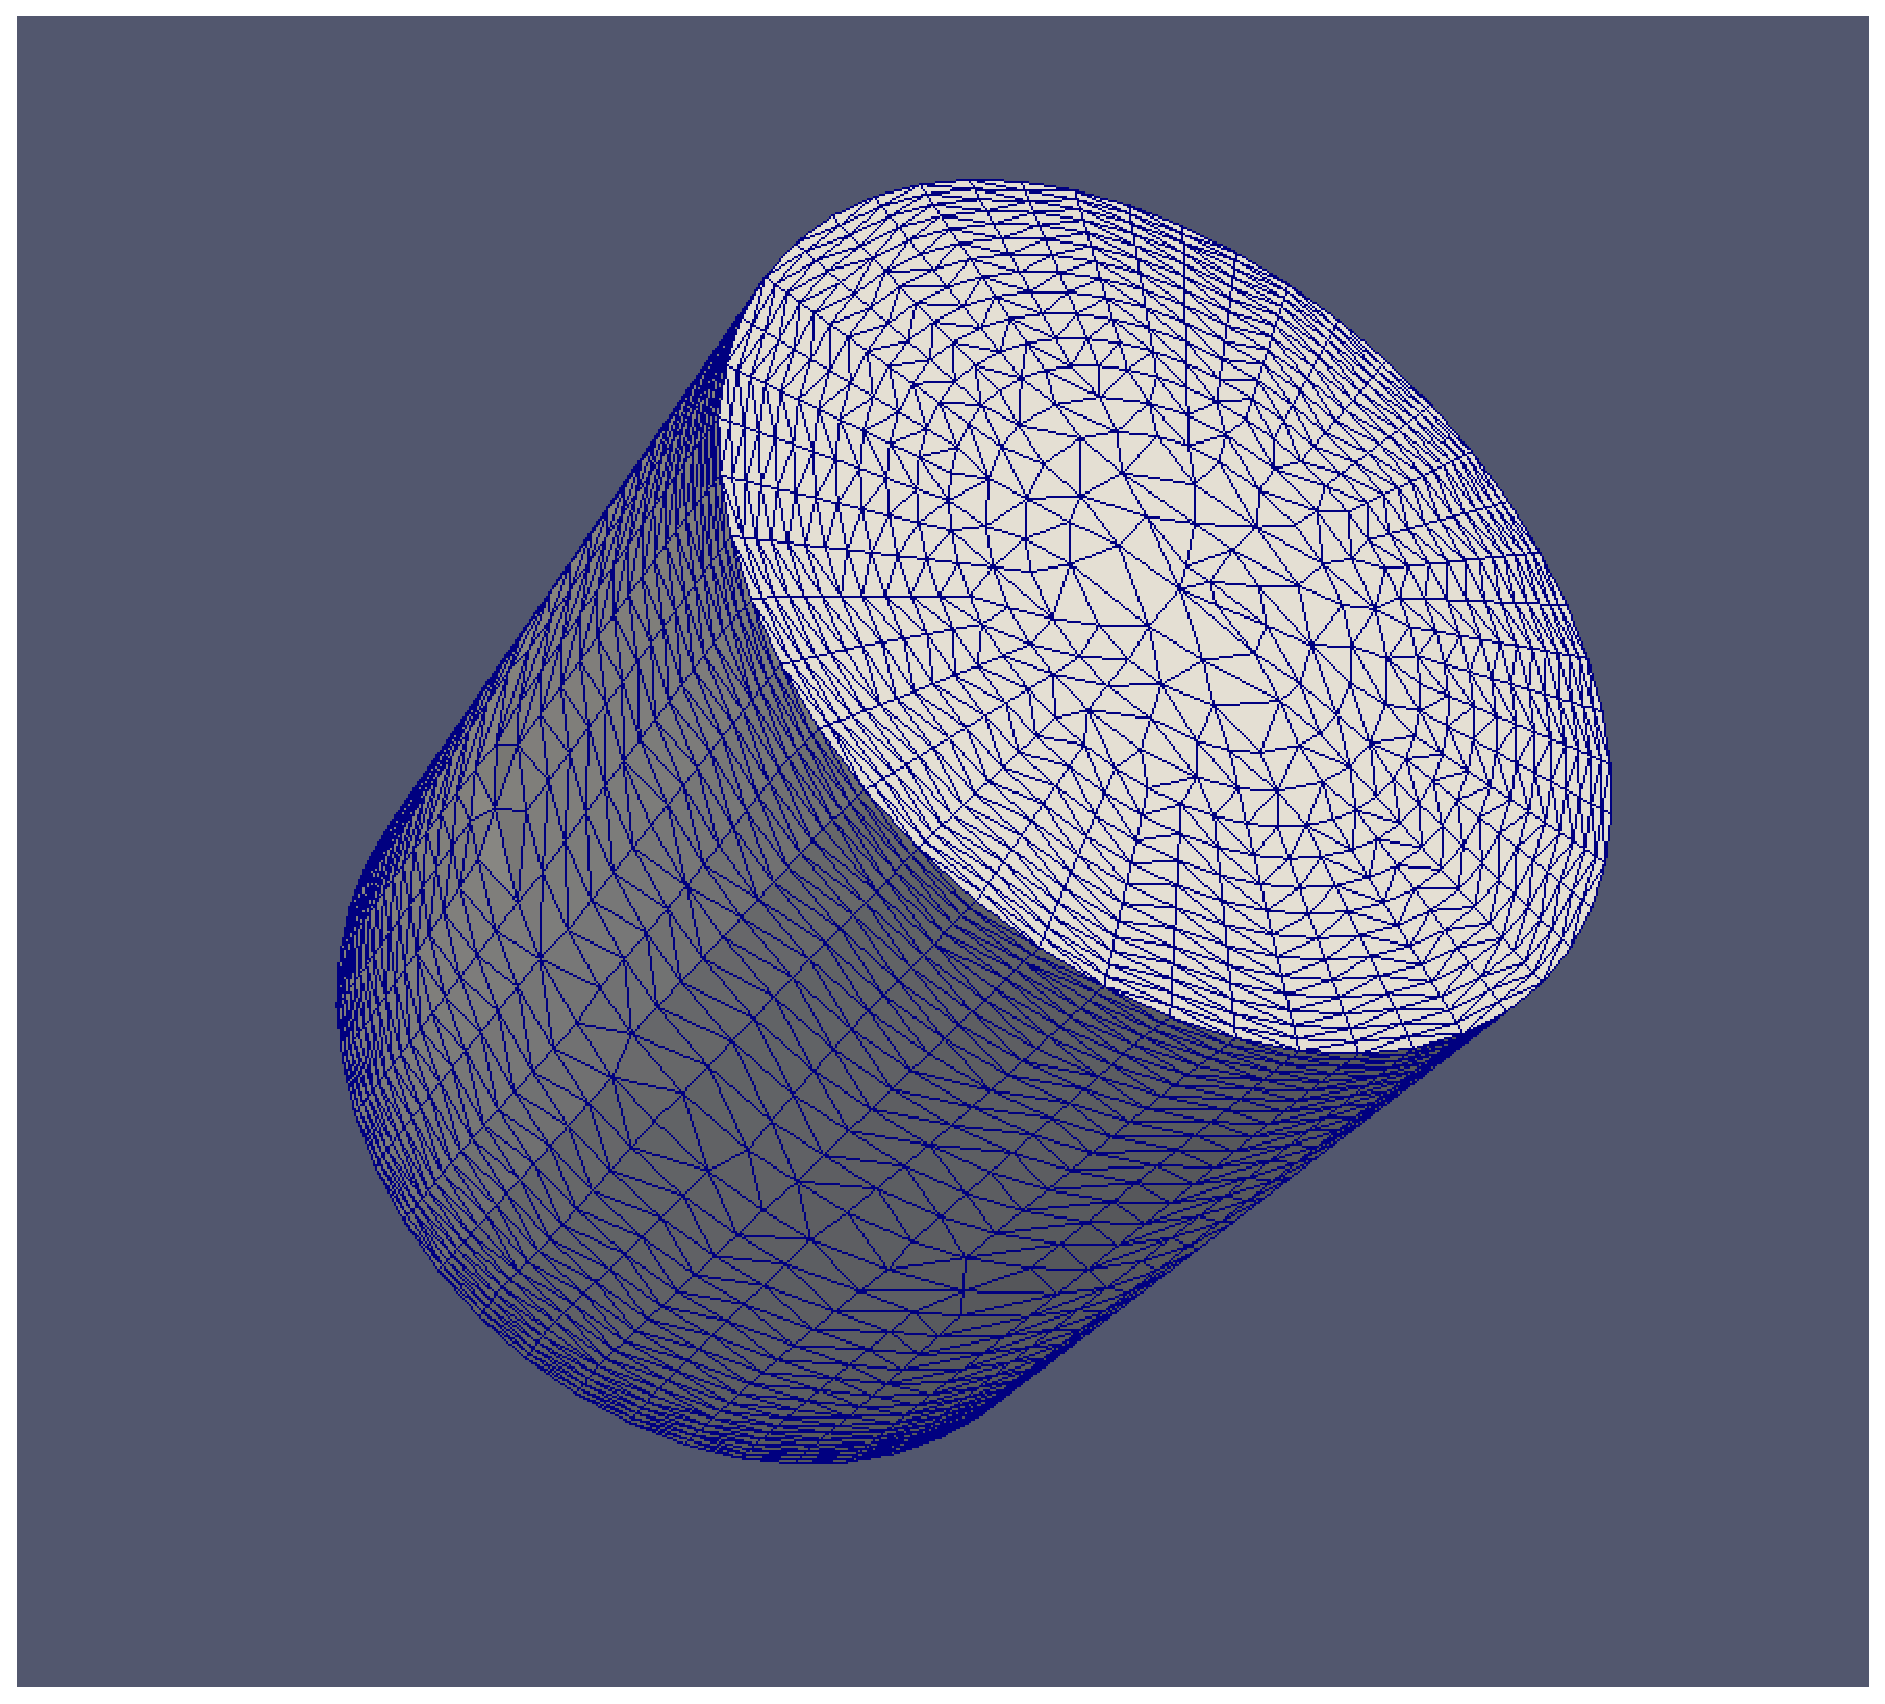
\includegraphics[width=.9\linewidth]{cylinder/fine/cyl-fine-mesh.eps}
  \caption{}
  \label{cyl-fine-mesh}
\end{subfigure}
\caption{Advancing layer mesh produced for a cylindrical object with finer boundary discretization. The boundary curve is preserved as the advancing layers march on the surface of the object.}
\label{cylinder-fine}
\end{figure}

\begin{table}
\caption{\label{cyl-table} Mesh parameters for Cylindrical Surface Mesh}
\centering
\begin{tabular}{lccccc}
\hline
%& Transition& & \multicolumn{2}{c}{}\\\cline{2-2}
Case& Edge length& Initial Extrusion Length & Growth Ratio & Aspect Ratio & No. of layers\\\hline
Coarse Boundary& 3.06 & 0.50 & 1.2 & 6.14 & 9\\
Fine Boundary& 1.34 & 0.24 & 1.1 & 5.57 & 16\\
\hline
\end{tabular}
\end{table}

\begin{figure}[hbt!]
\centering
\begin{subfigure}{.5\textwidth}
  \centering
  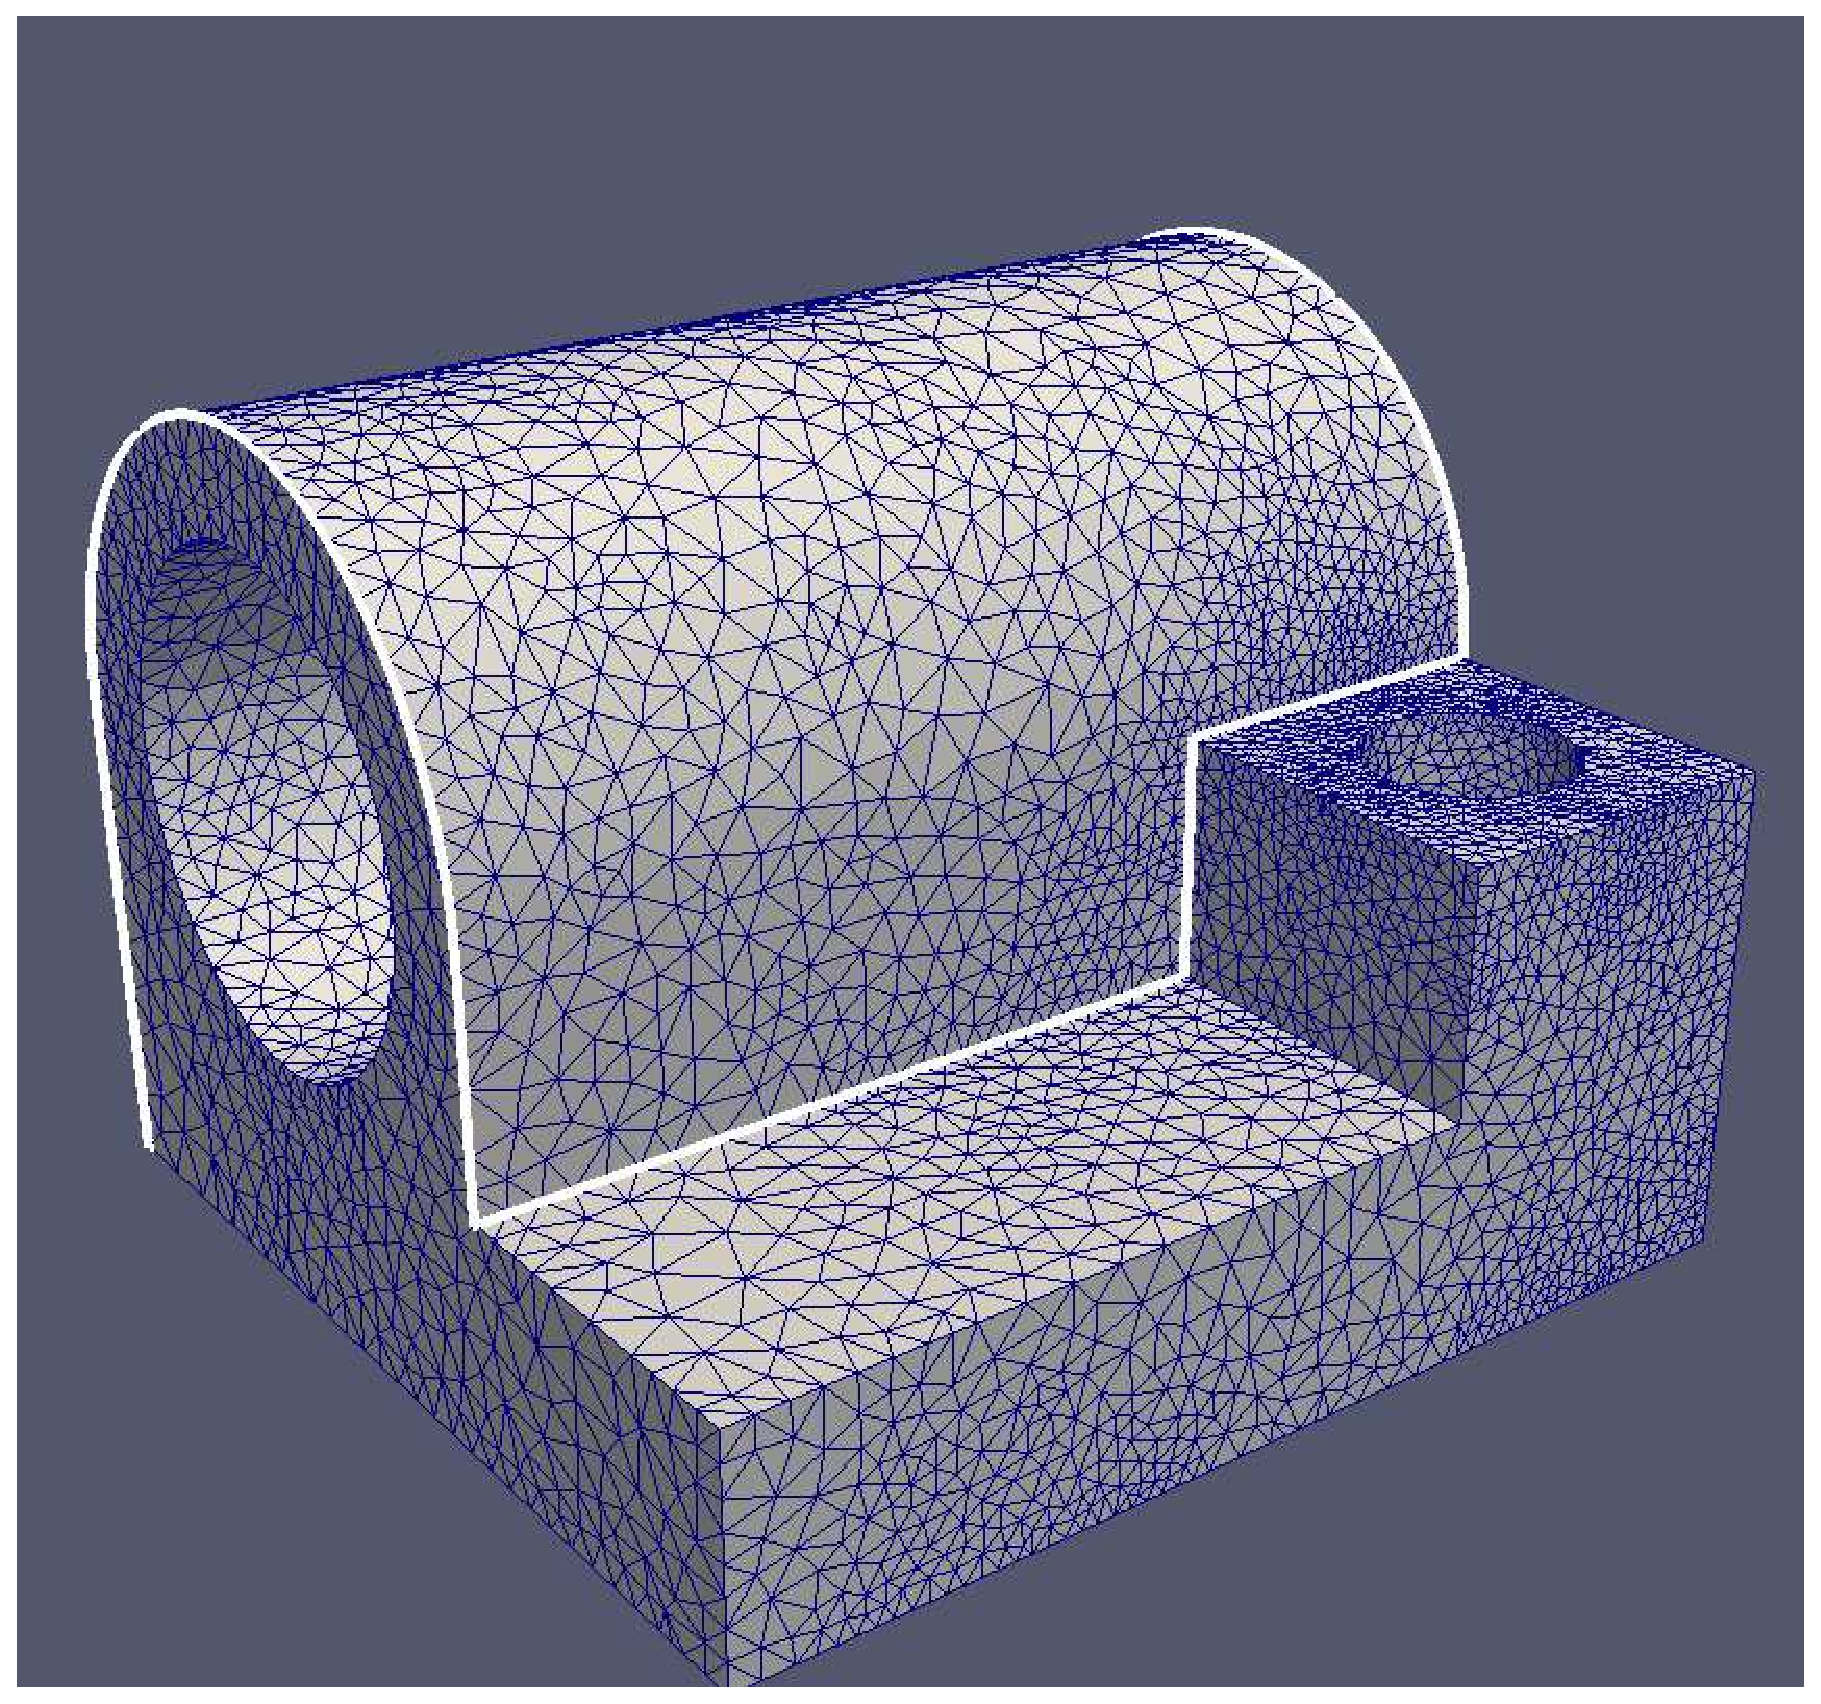
\includegraphics[width=.9\linewidth]{joint-surf5/before1.eps}
  \caption{}
  \label{surf5-joint-view1}
\end{subfigure}%
\begin{subfigure}{.5\textwidth}
  \centering
  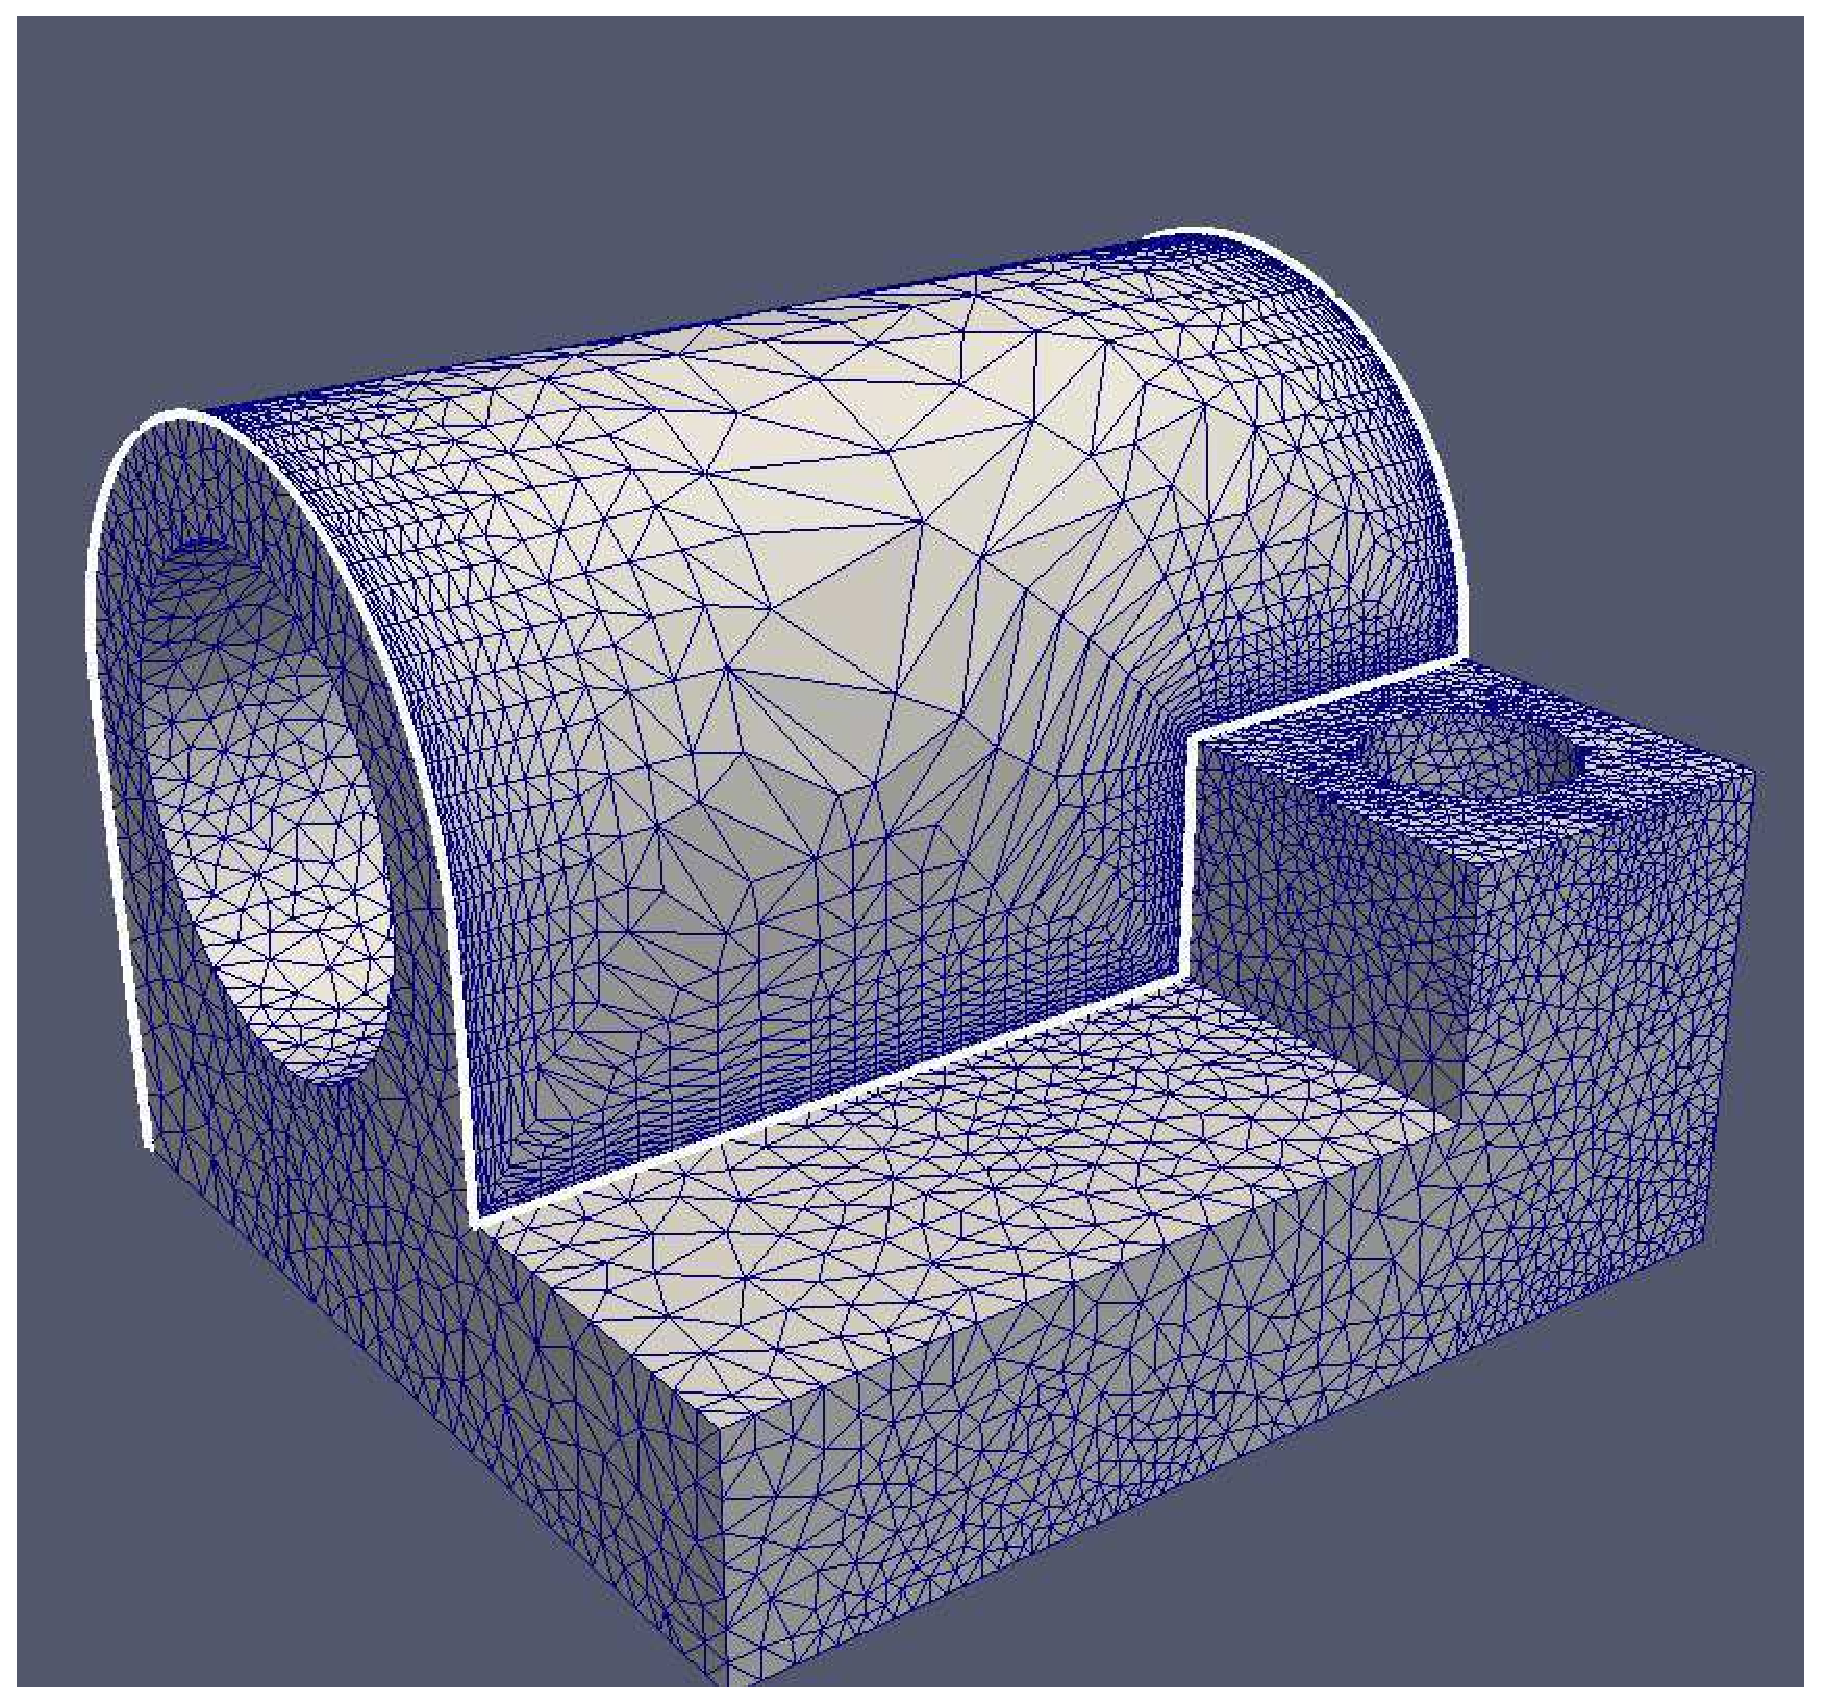
\includegraphics[width=.9\linewidth]{joint-surf5/after1.eps}
  \caption{}
  \label{surf5-joint-view2}
\end{subfigure}
\begin{subfigure}{.5\textwidth}
  \centering
  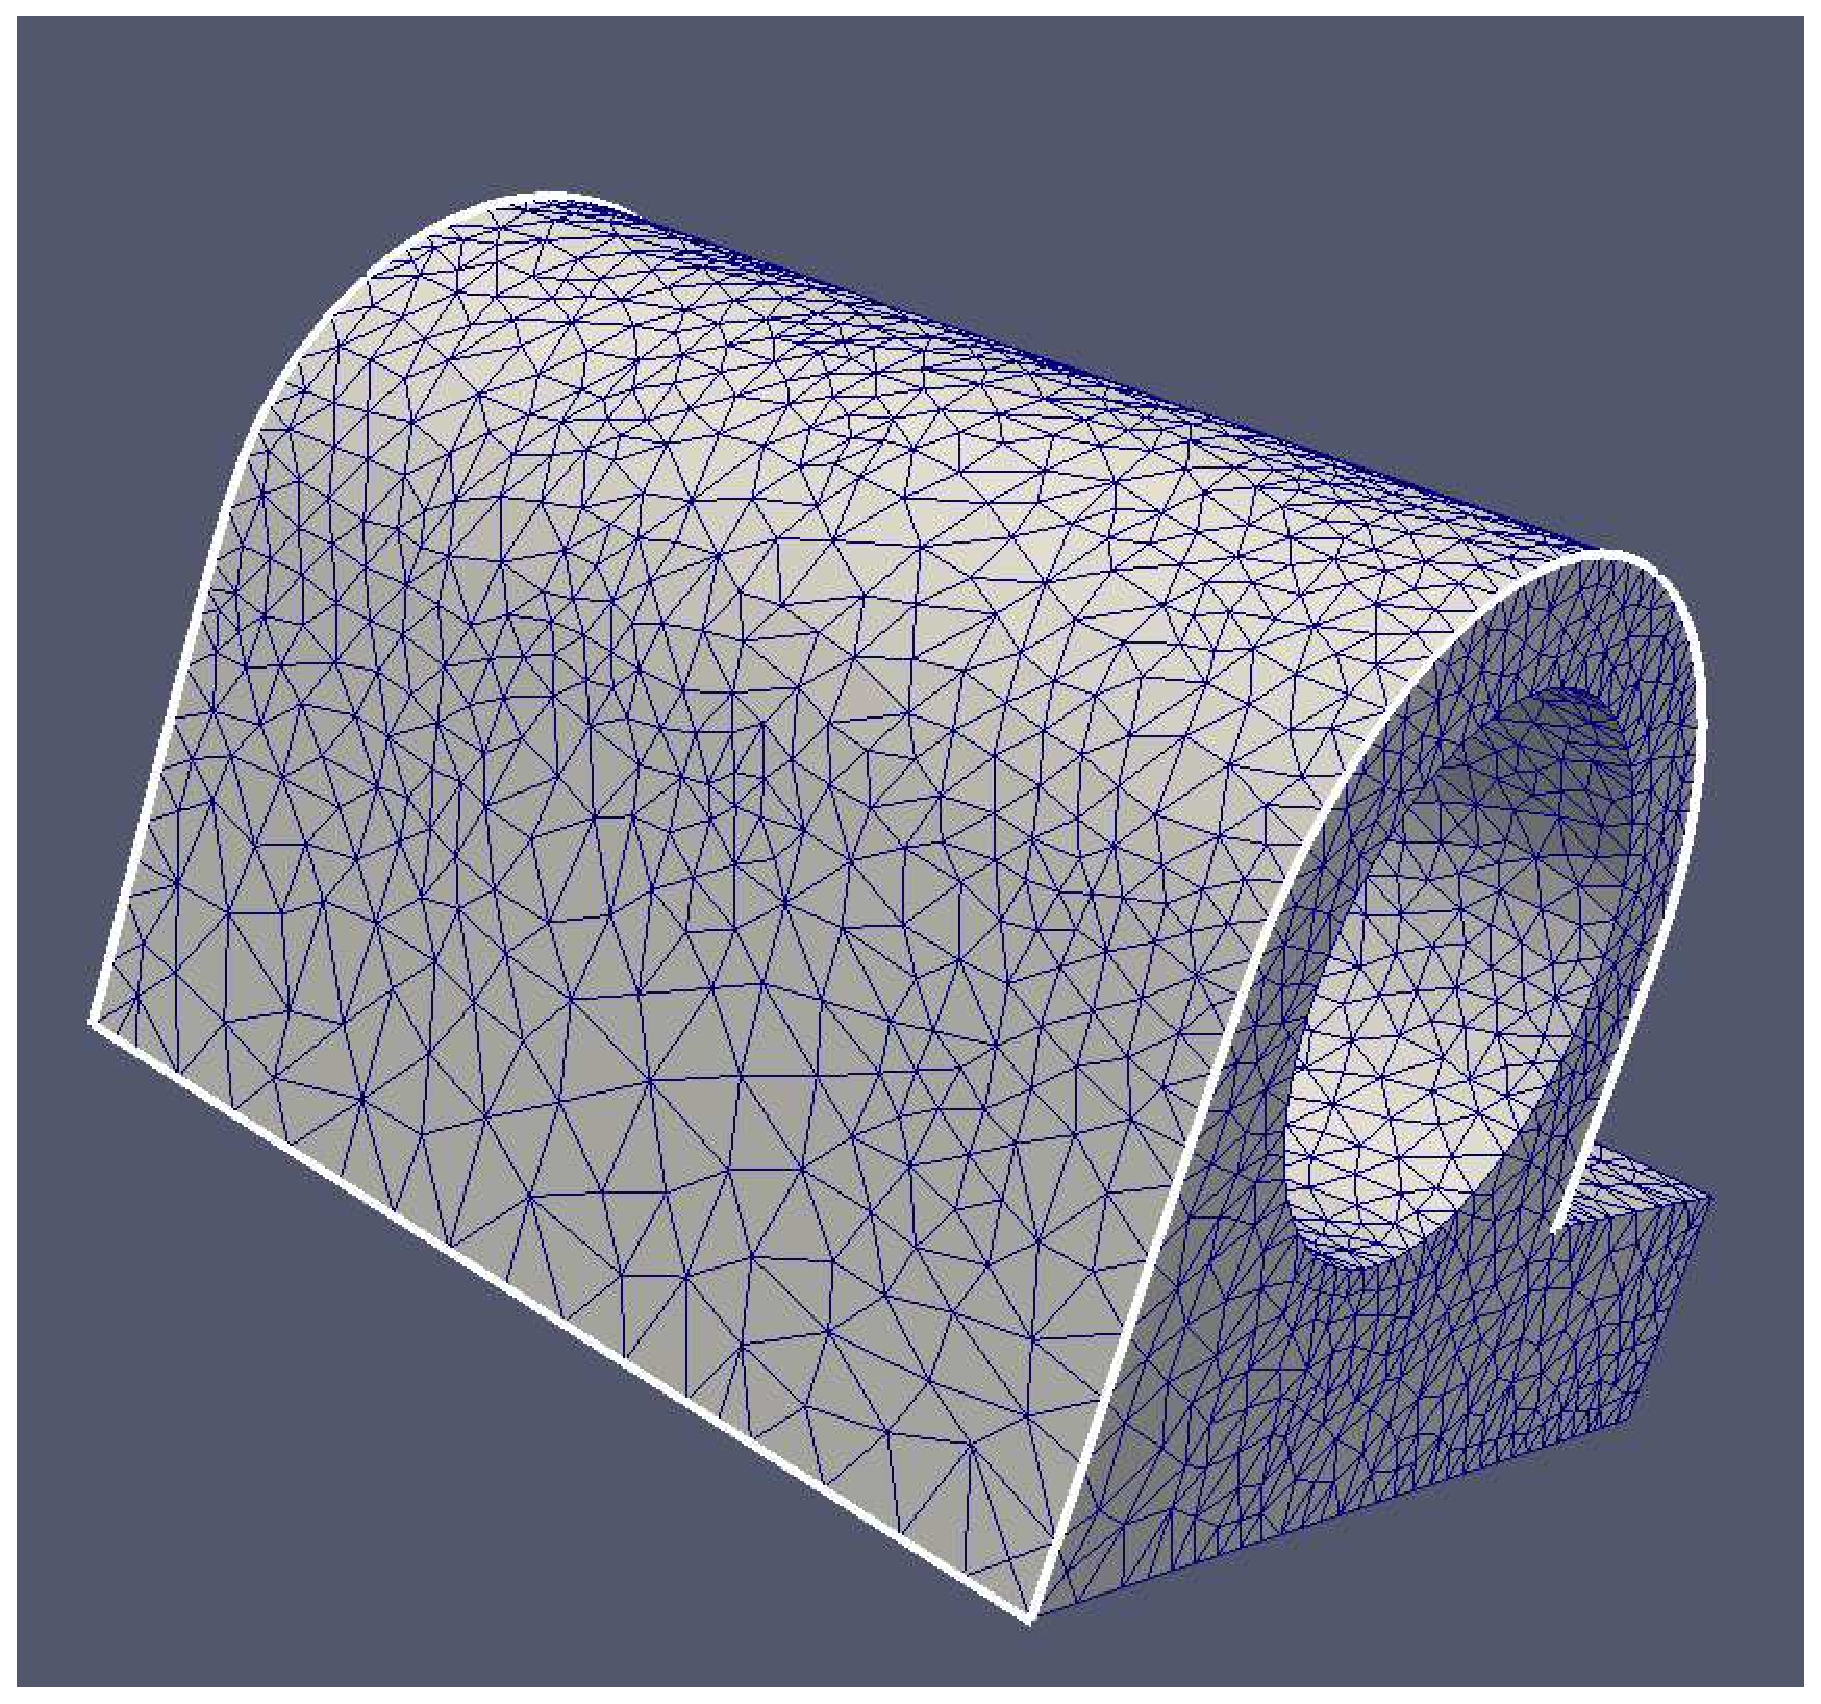
\includegraphics[width=.9\linewidth]{joint-surf5/before2.eps}
  \caption{}
  \label{surf5-joint-view3}
\end{subfigure}%
\begin{subfigure}{.5\textwidth}
  \centering
  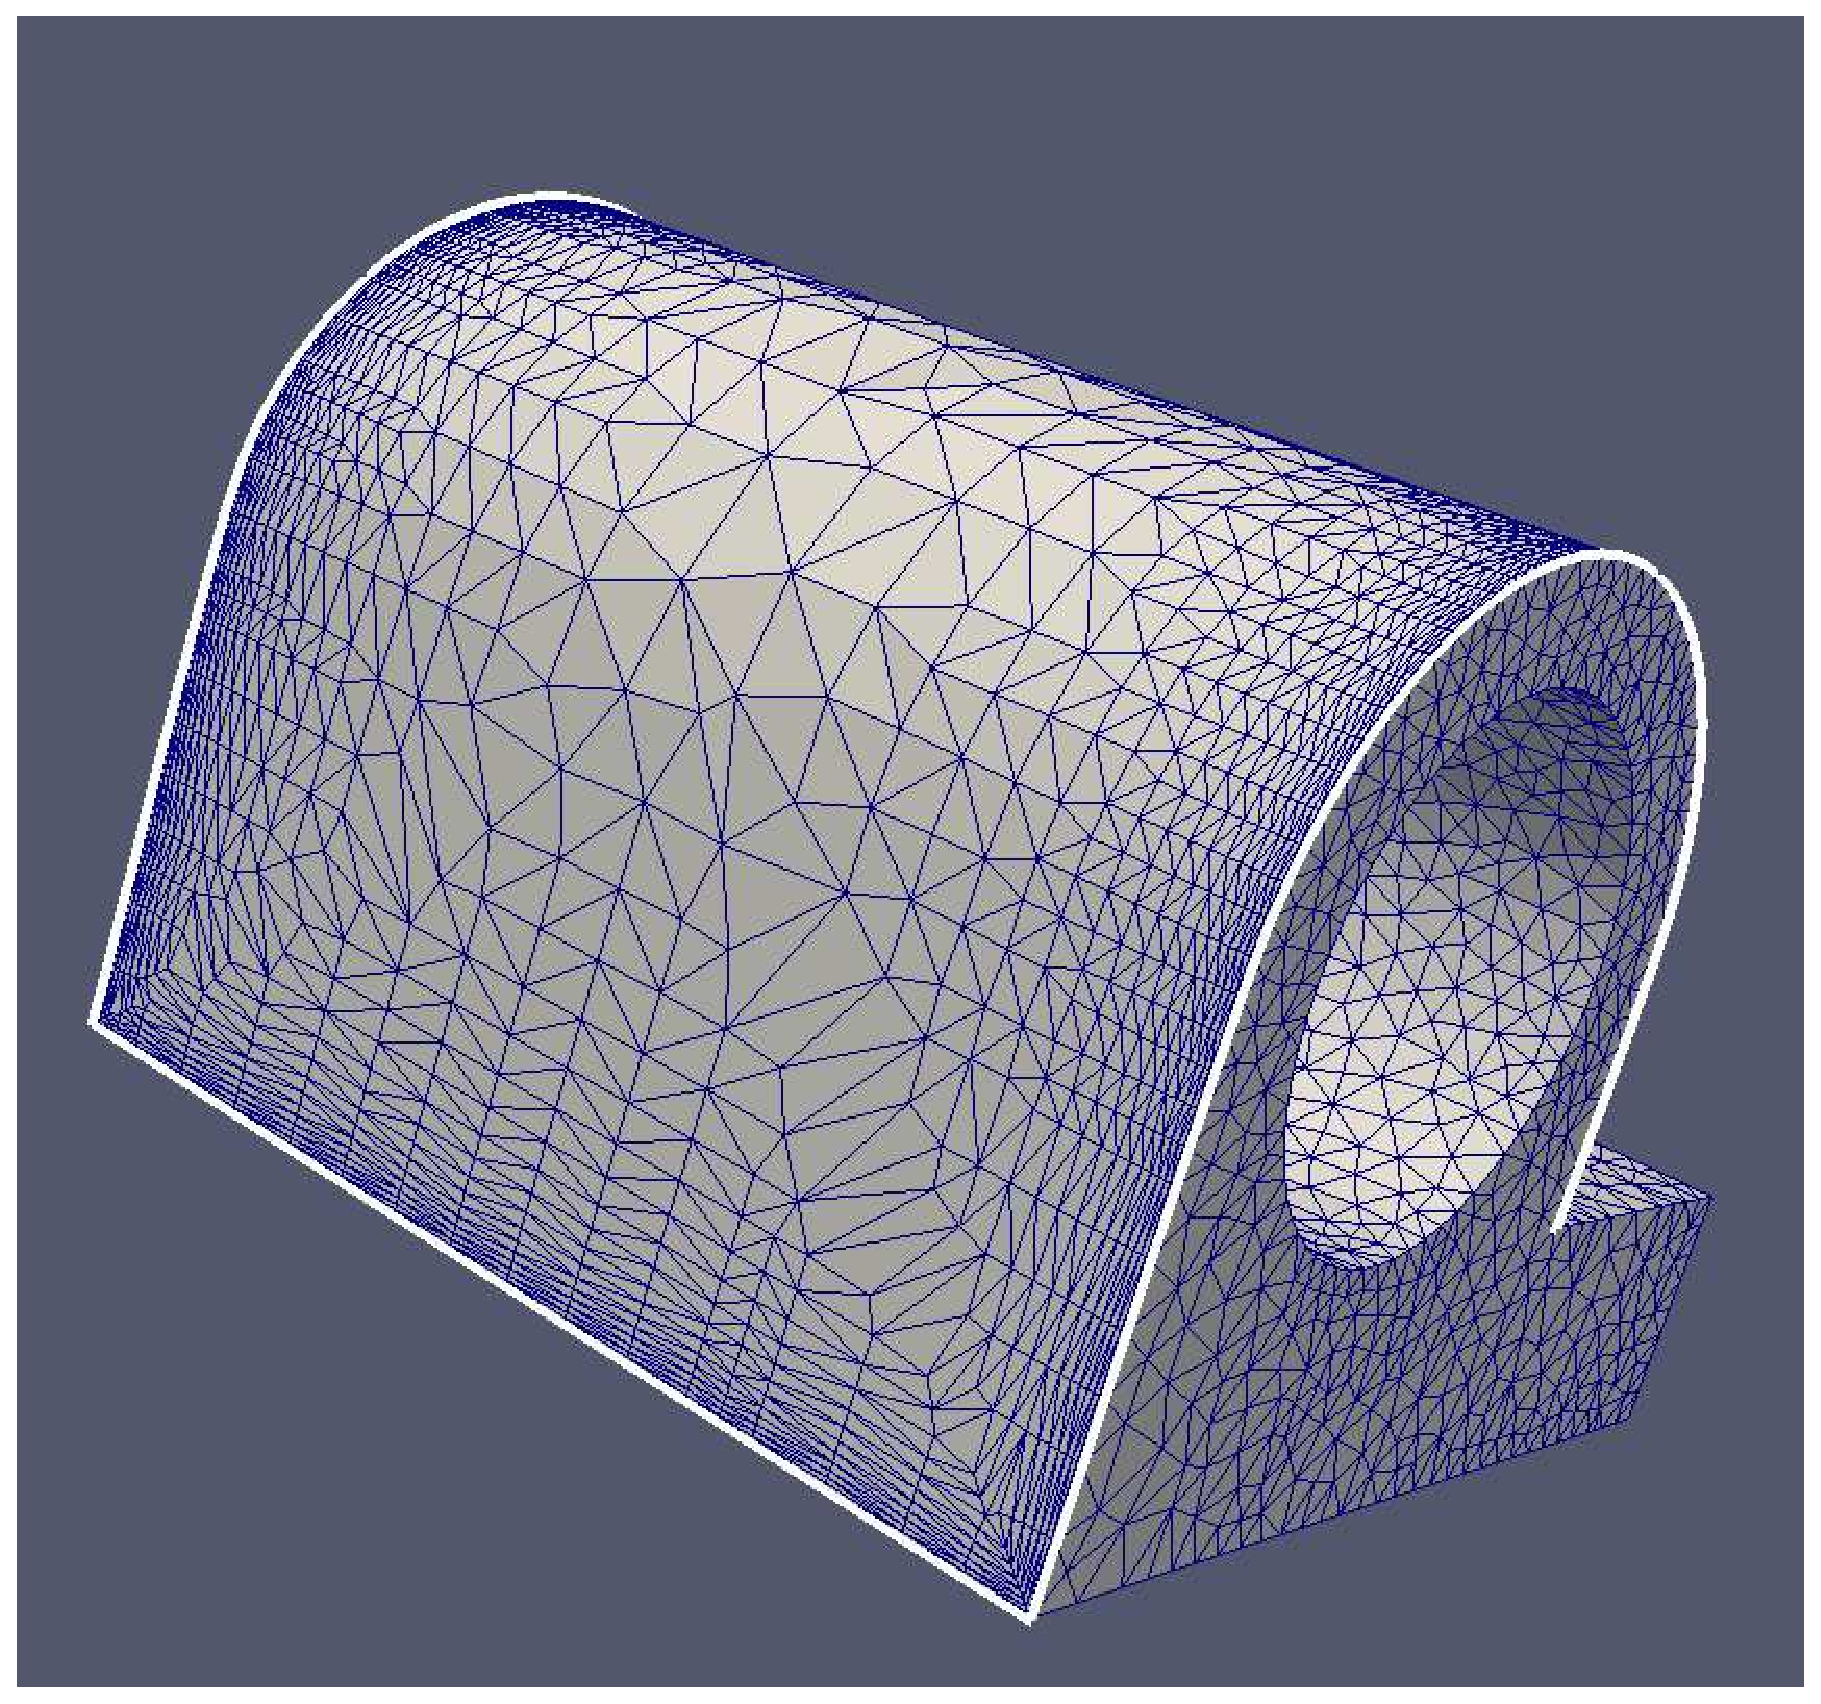
\includegraphics[width=.9\linewidth]{joint-surf5/after2.eps}
  \caption{}
  \label{surf5-joint-view4}
\end{subfigure}
\caption{One of the surfaces of the geometry remeshed with the advancing layer surface mesh generation algorithm. The boundary of the surface is highlighted.}
\label{joint-surf5}
\end{figure}

\begin{figure}[hbt!]
\centering
\begin{subfigure}{.5\textwidth}
  \centering
  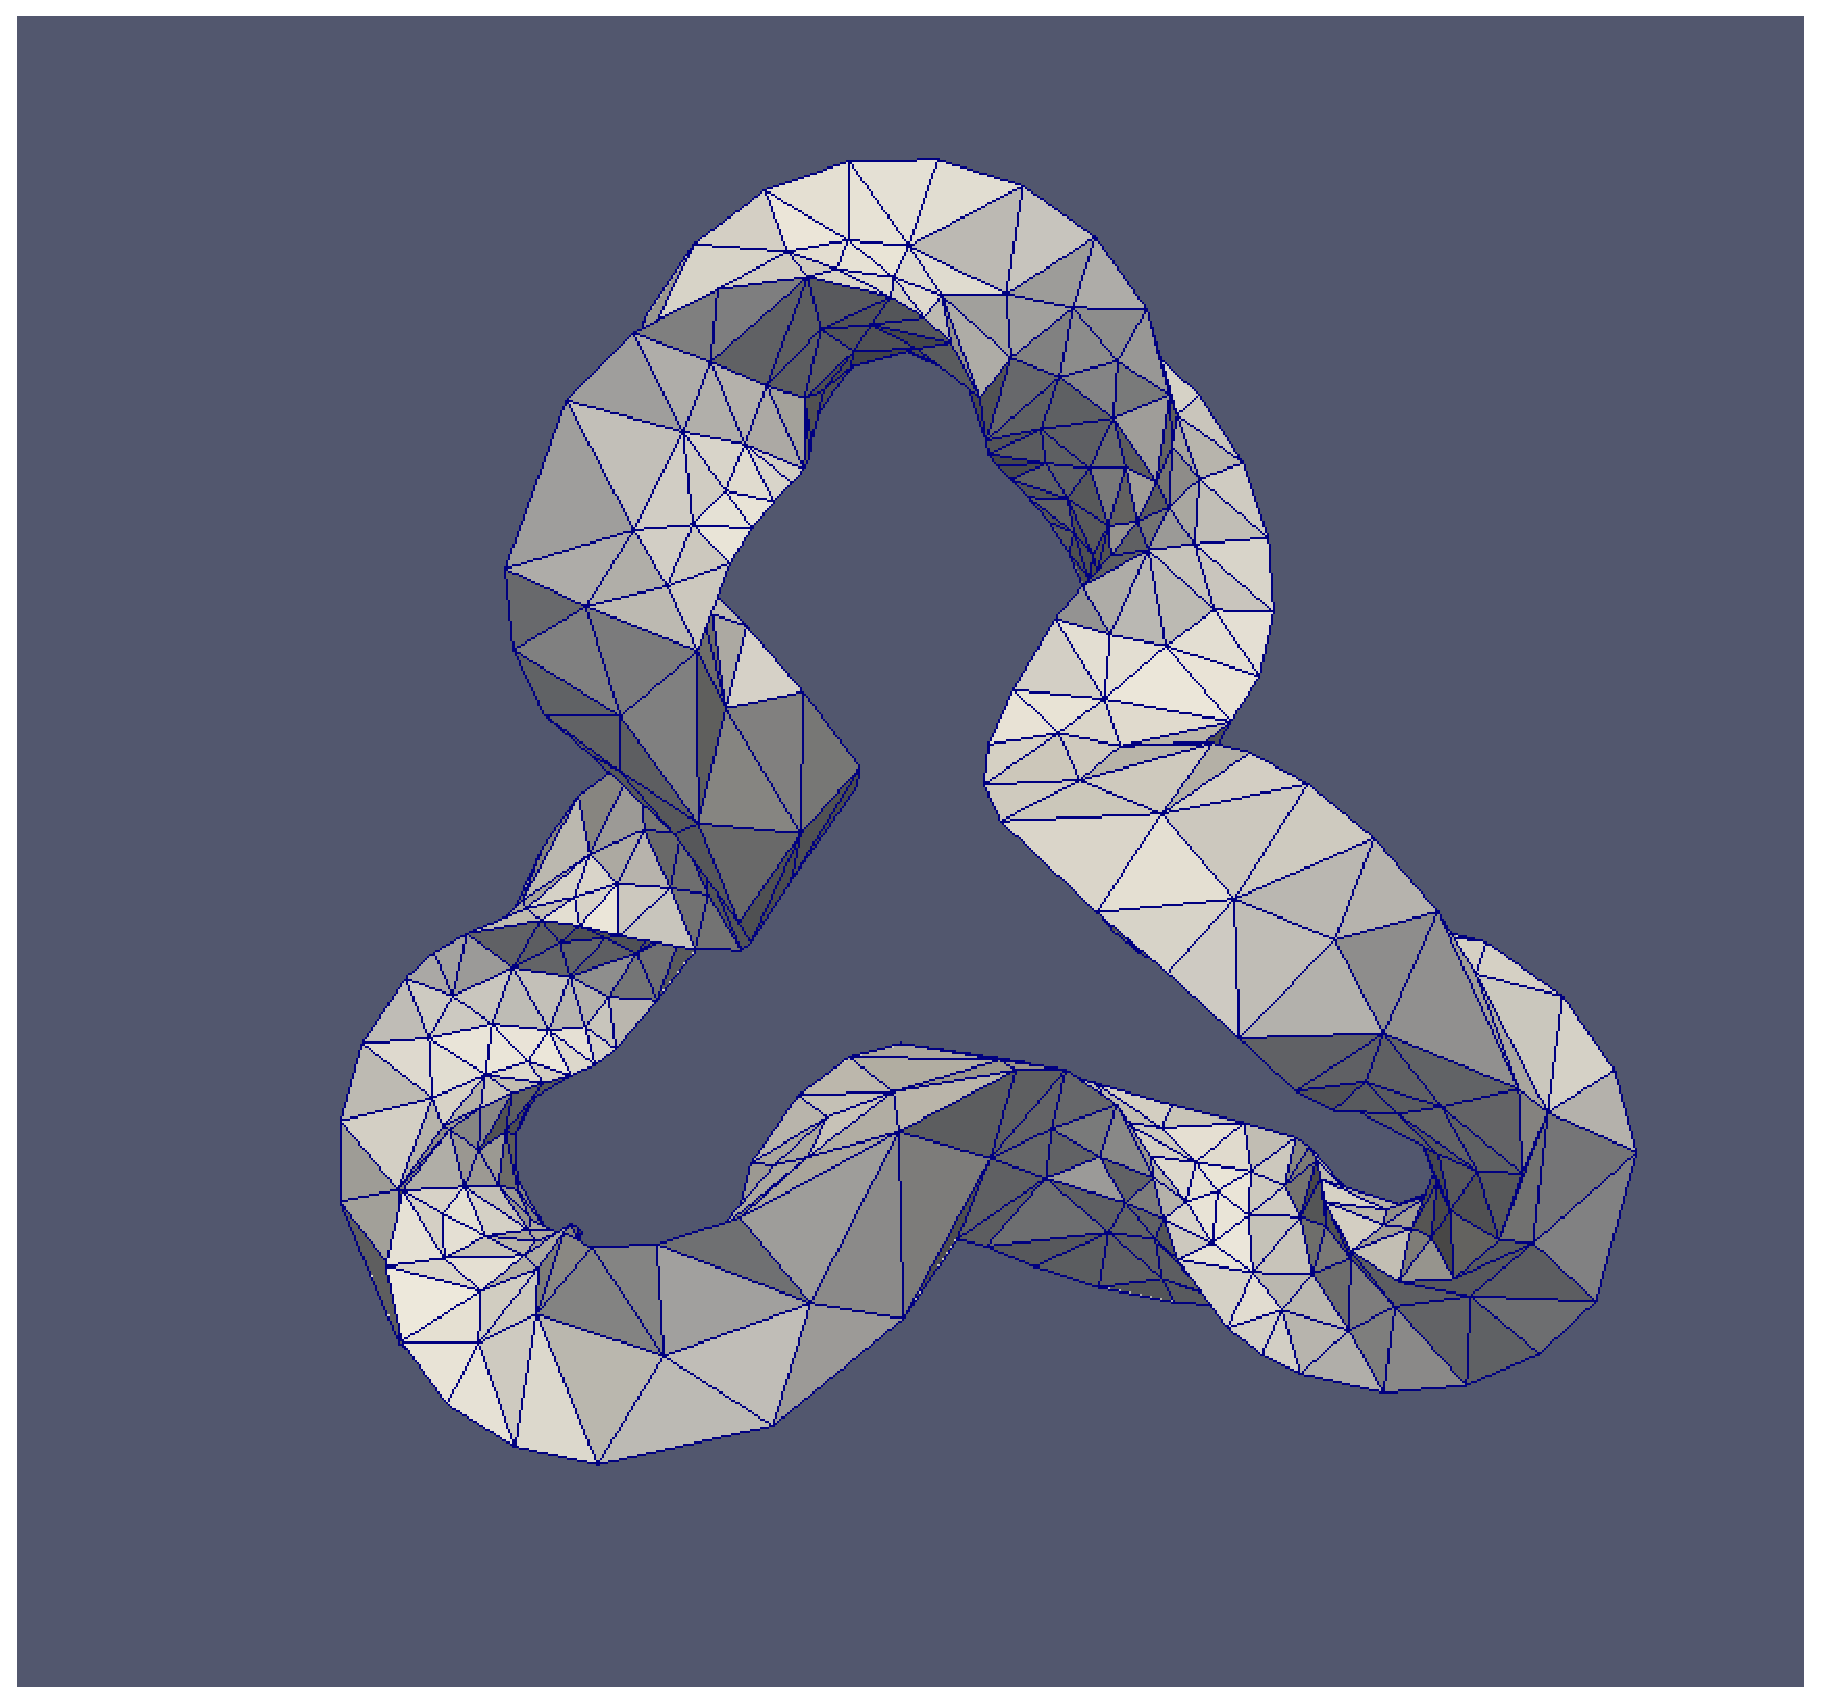
\includegraphics[width=.9\linewidth]{twist/before.eps}
  \caption{}
  \label{twist1}
\end{subfigure}%
\begin{subfigure}{.5\textwidth}
  \centering
  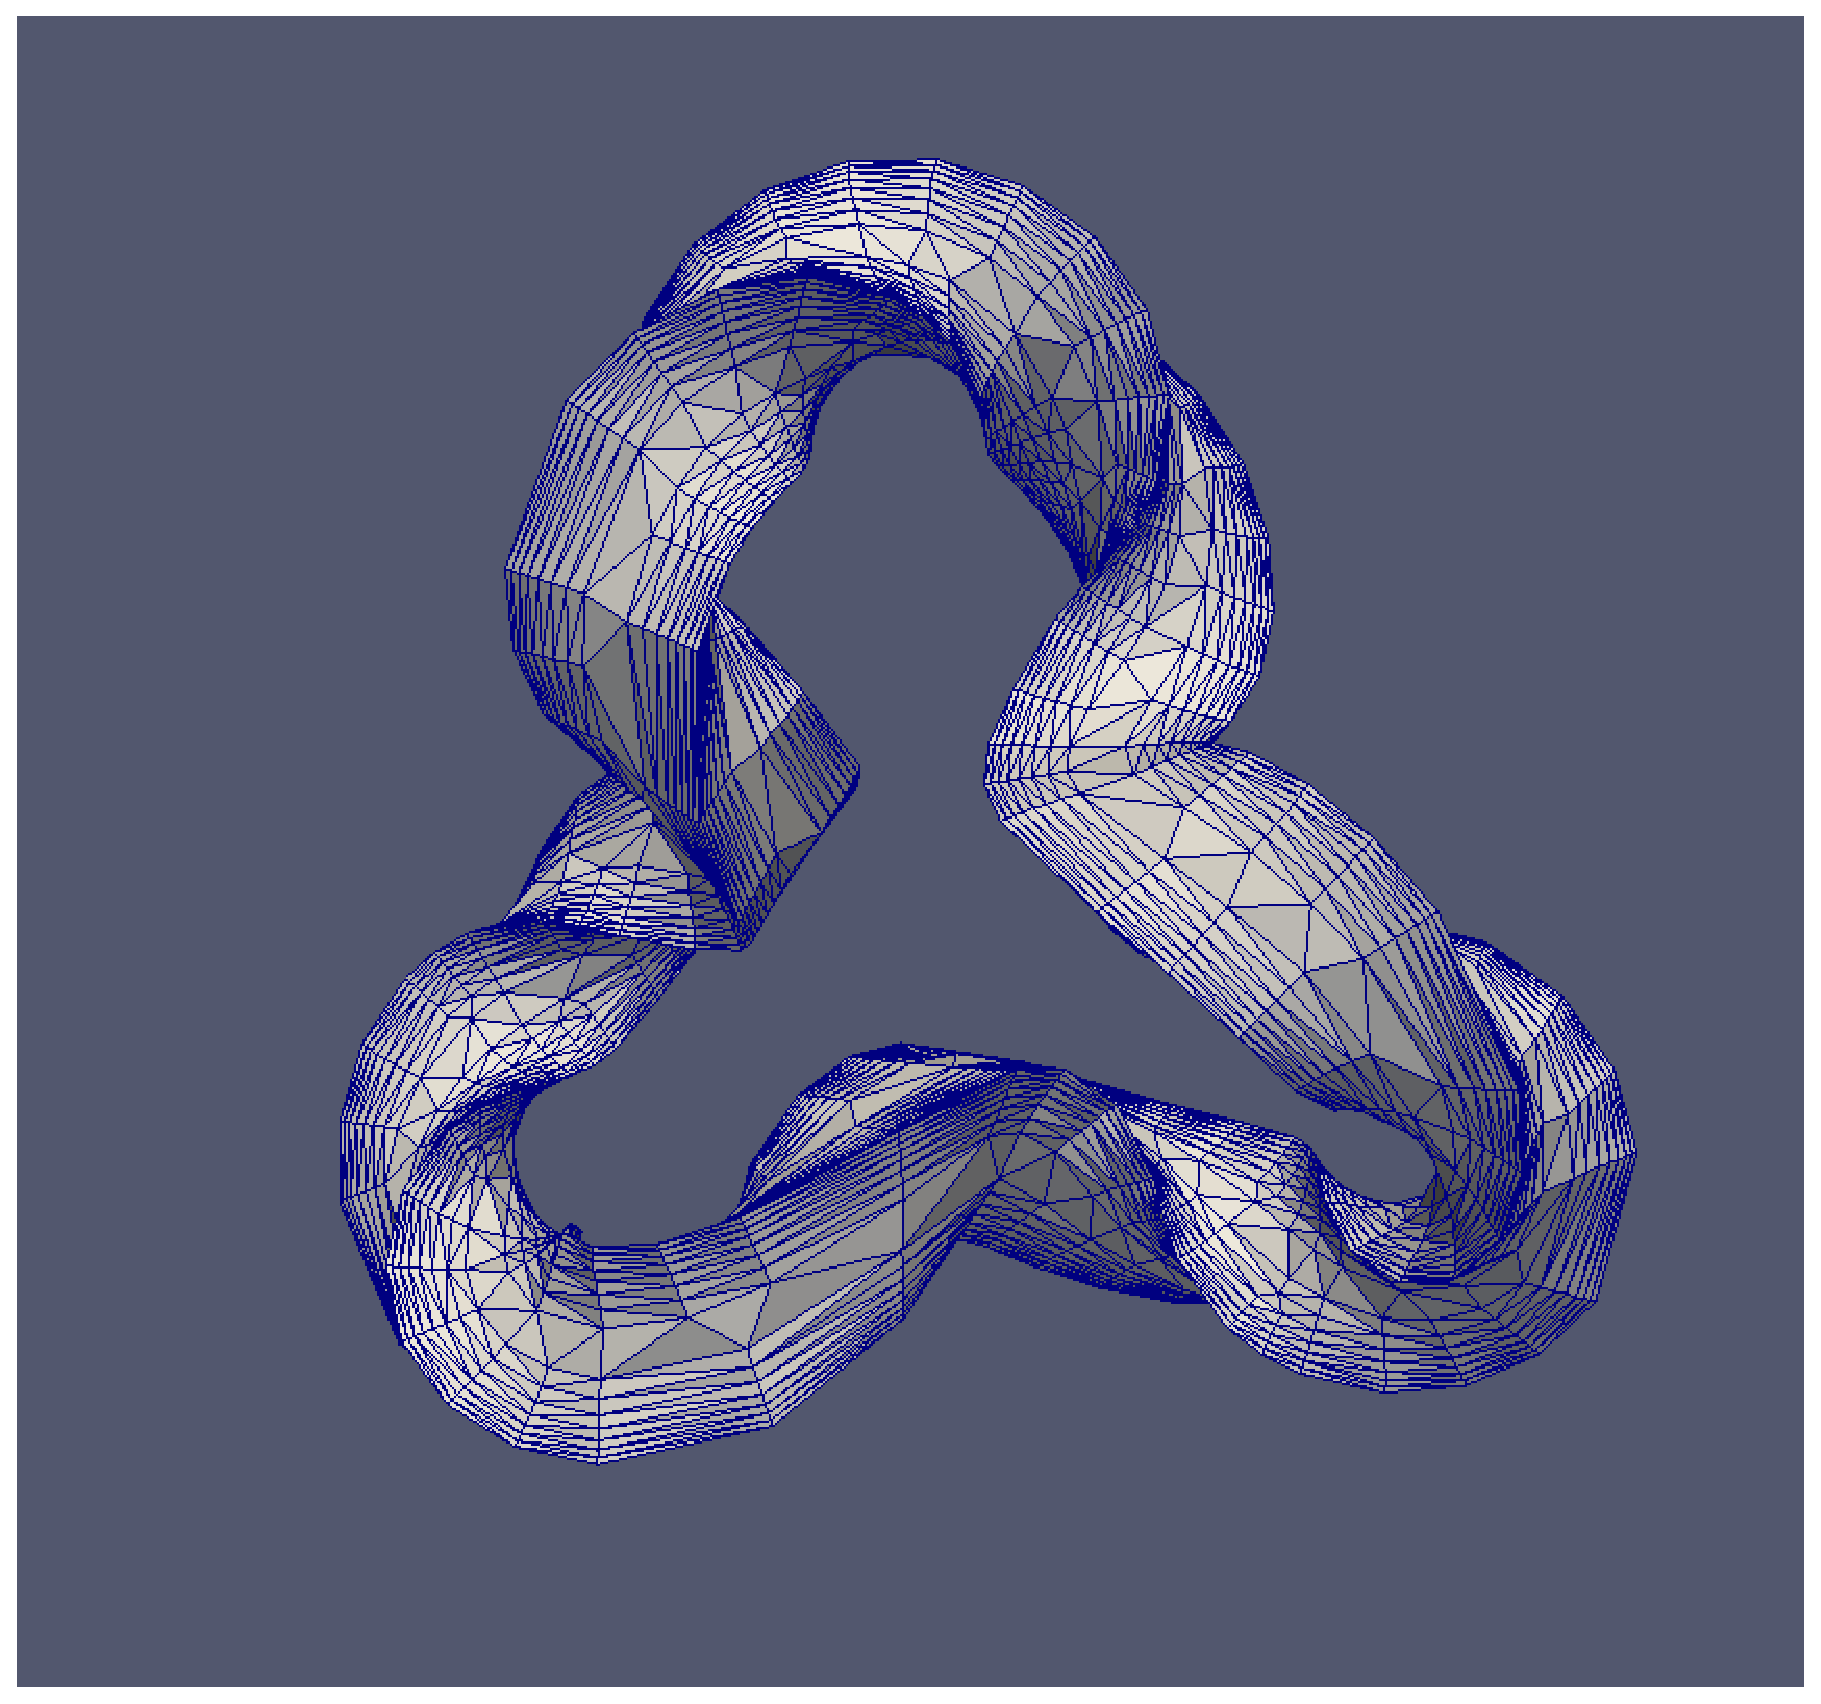
\includegraphics[width=.9\linewidth]{twist/after.eps}
  \caption{}
  \label{twist2}
\end{subfigure}
\begin{subfigure}{.5\textwidth}
  \centering
  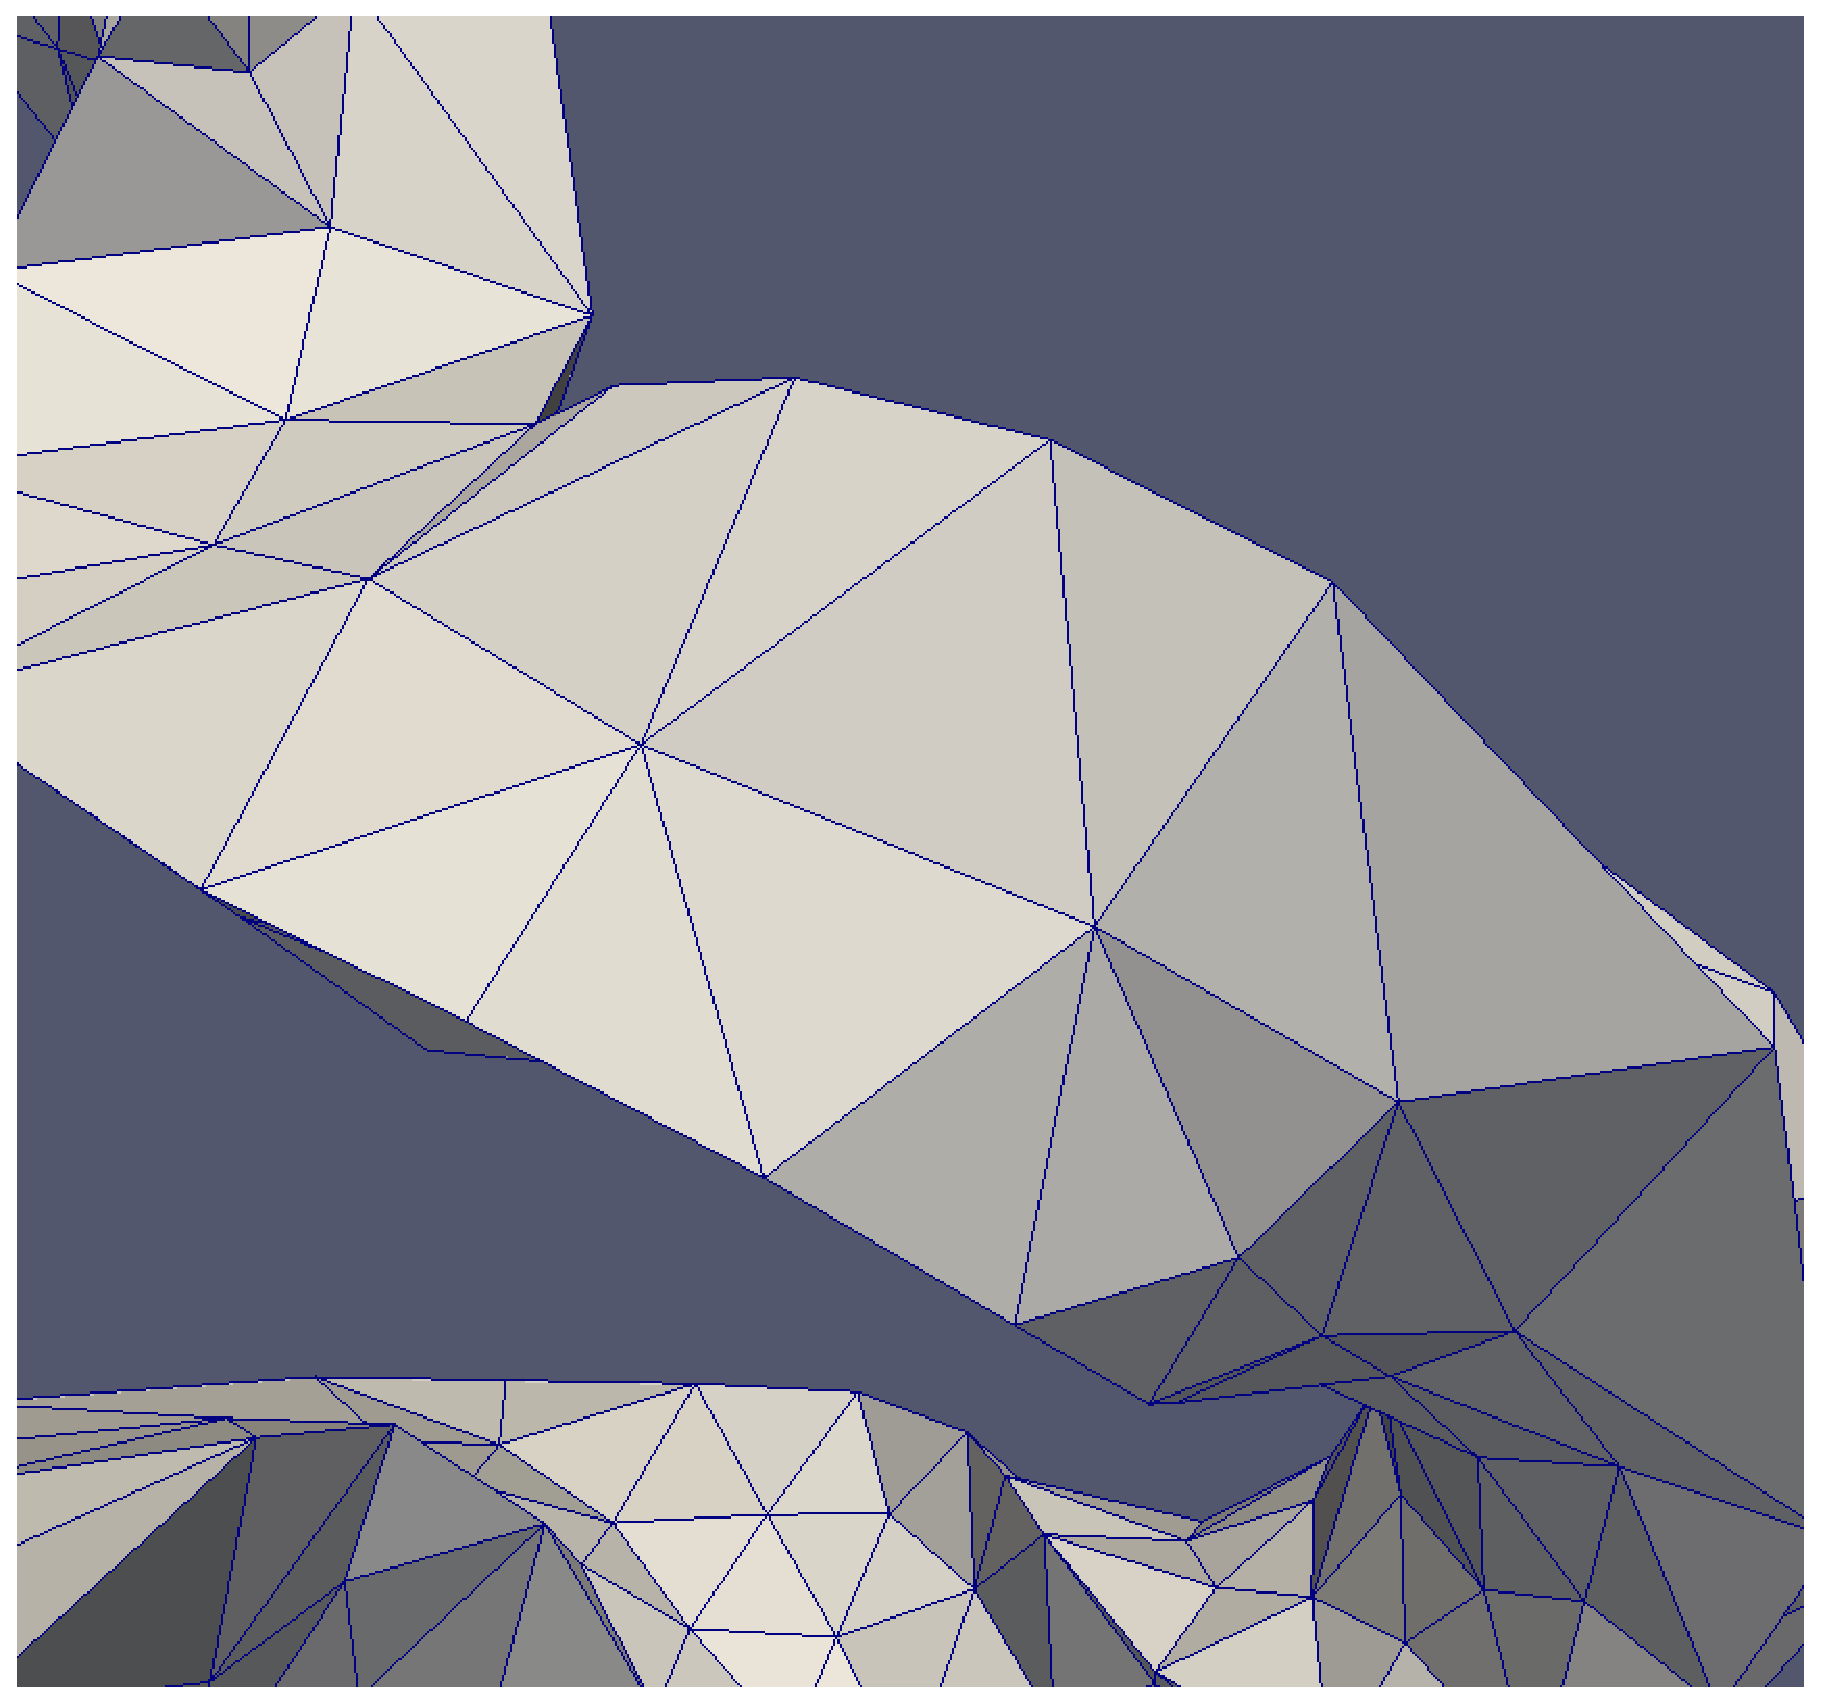
\includegraphics[width=.9\linewidth]{twist/before1.eps}
  \caption{}
  \label{twist3}
\end{subfigure}%
\begin{subfigure}{.5\textwidth}
  \centering
  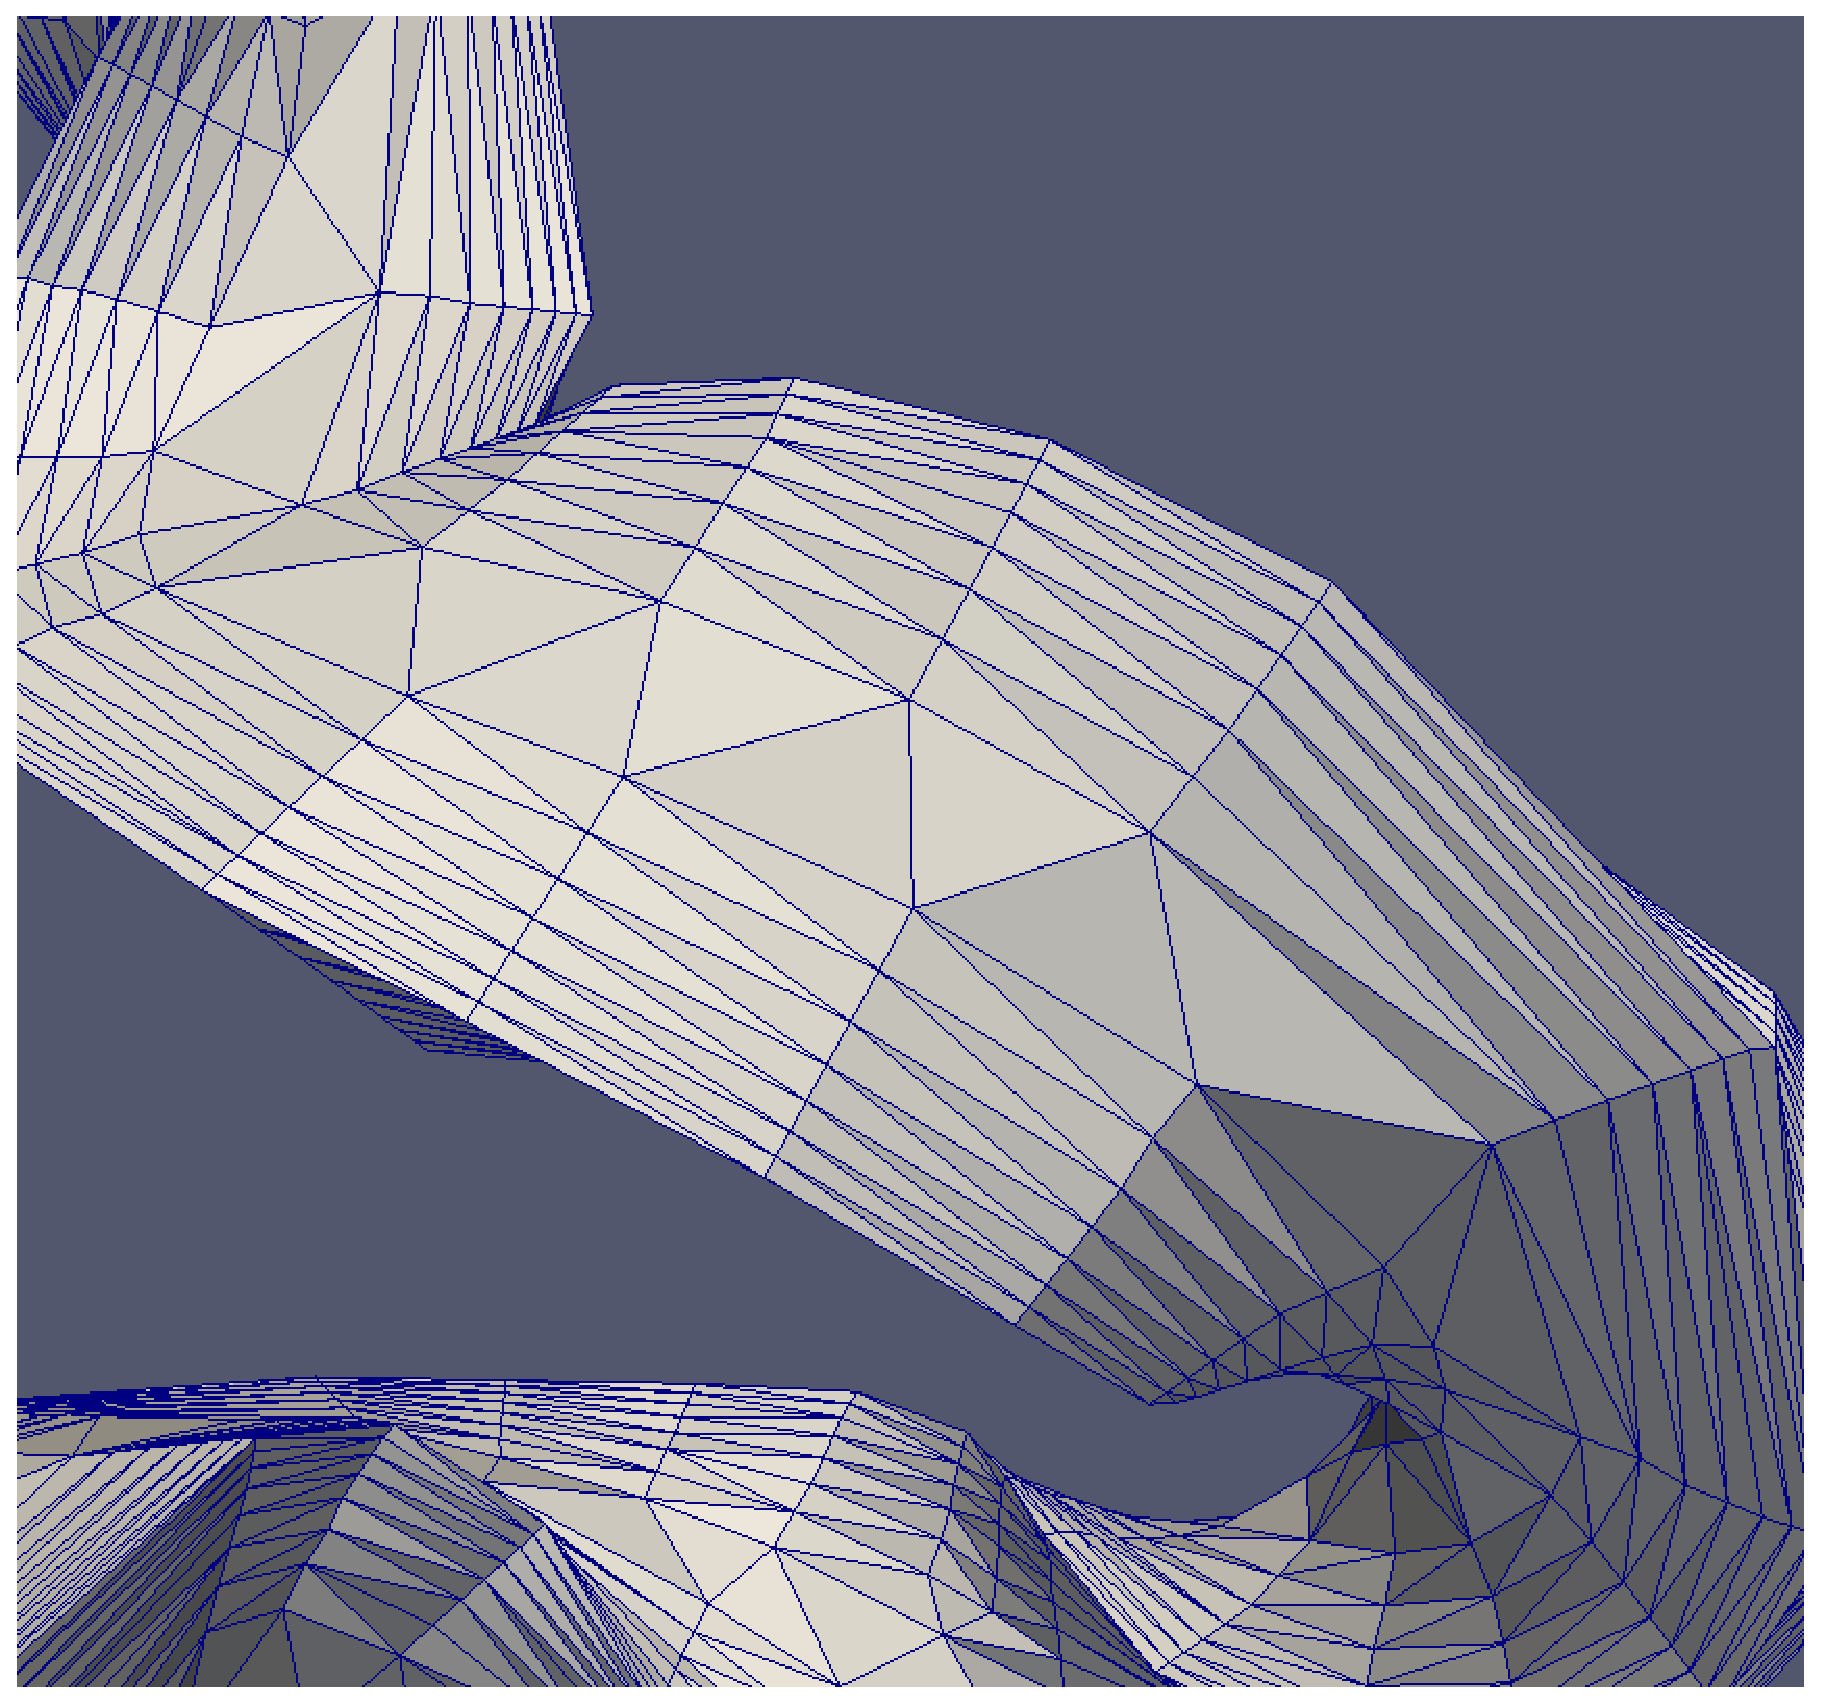
\includegraphics[width=.9\linewidth]{twist/after1.eps}
  \caption{}
  \label{twist4}
\end{subfigure}
\caption{A contorted initial geometry is meshed using the advancing layer algorithm for seven layers. The boundaries of the geometry are preserved even after advancing for several layers into the surface of the object.}
\label{twist}
\end{figure}

\section{Work Plan for Complete Paper}

In the final paper, we would present examples of completed surface meshes for more complex geometries. The following objectives would be met to achieve that.

\begin{itemize}
    \item Merge pairs of triangles to form quads. This would be relatively easy as a front edge with a proper descent defines a quad.
    \item Add more than one extrusion points to convex corners of the geometry to make the initial aspect ratio of the advancing front more uniform.
    \item Add robustness to the front collision and redefinition routine so as to handle geometries with complex features and sharp concave corners.
    \item Identify or take user input for the direction of anisotropy at each extrusion point on the advancing layer.
    \item Add smoothing based on spring force model. The smoothing would help to ensure that the aspect ratio of the mesh elements remain consistent along the advancing front. It would also ensure that the mesh elements generated deviate as little from the underlying surface as possible.
    \item Vary extrusion length at a point with the angle between its adjacent edges on the advancing front
\end{itemize}

\begin{comment}
\section{Examples}

We use the surface mesh generation technique described above to mesh some simple geometries. Three of the cases for which we produced a mesh are described here. We also present the mesh parameters for each mesh. These include the number of points, number of triangles, number of quads, and the number of edges in the mesh. The mesh quality is also assessed for all the meshes. We report the maximum angle in each mesh and the bar-graph representing the distribution of the angles in the mesh. Mesh quality parameters for the input surface triangulation are also shown. In the regions of the mesh where we desire high-aspect ratio, these mesh quality parameters, i.e., angles of the mesh are not a good reference. Here, we ideally need a well structured mesh with good refinement along the surface normal. Hence, minimum or maximum angle in the mesh is not the best criteria to evaluate the quality of the mesh. We show the figures of such meshes to highlight the desired features in the mesh.

\subsection{Test Case 1: Hook}

\emph{Here, I can demonstrate the layer generation in the hook's long cylindrical surface with a couple of figures. Also, the generation of layers in the flat ends of the hook. I can also demonstrate vertex removal from the interior of the mesh. Showing the surface normals can also be considered. I will make decisions on these things while writing this section.}

\subsection{Test Case 2: Joint}

\emph{I can demonstrate that the underlying geometry is farily coarse and is badly triangulated. Ten different surfaces need to be meshed having a range of geometric complexities. Generation of layers in the interior cylindrical and the surface with a hole can be highlighted. The generation of rings around the hole demonstrate the high quality boundary representation in the mesh. If layer collapse works well, include that here. Figures showing edge recovery after layer generation and front redefinition would be useful too.}

\subsection{Test Case 3: Airfoil}

\emph{I would like to demonstrate a simple airfoil case. Maybe extrude NACA0012 in 3d(Is it available with us?). I am confused whether I should change the boundary representation in this case so as to mark specific boundaries only for extrusion? Or for now, I can just extrude from all the boundaries and then in the future(after abstract) come back to redefine boundary which will be extruded.}

\section{Future Work}

\emph{Just for Outline. Needs to be changed.}

\section{Conclusion}

% \section*{Appendix}

% \emph{I might use this section to add the pseudo code for concepts in the surface mesh or parameters used for developing the meshes included in the results section}

\section*{Acknowledgments}

\end{comment}


\bibliography{sample}

\end{document}
